\documentclass[12pt,a4paper,oneside]{report}

% --- Packages fondamentaux ---
\usepackage[utf8]{inputenc}
\usepackage[T1]{fontenc}
\usepackage[french]{babel}
\usepackage{mathptmx} % Police Times New Roman standard
\usepackage[margin=2.5cm,headheight=28pt]{geometry}
\usepackage{setspace}
\onehalfspacing
\usepackage{needspace}

% --- Mise en page des paragraphes ---
\setlength{\parindent}{0.8cm}
\setlength{\parskip}{6pt}

% --- Graphiques, tableaux et couleurs ---
\usepackage{graphicx}
\usepackage{xcolor}
\usepackage{tikz}
\usetikzlibrary{shapes,arrows,positioning,calc,fit,shadows,shapes.geometric,decorations.pathreplacing}
\usepackage{tabularx}
\usepackage{array}
\usepackage{booktabs}
\usepackage{colortbl}
\usepackage{float}
\usepackage{caption}
\usepackage{subcaption}
\usepackage{titlesec}
\usepackage{tocloft}
\usepackage{enumitem}

% ====================================================================
% CHARTE GRAPHIQUE — Fondation OCP (vert institutionnel) / EMSI (bleu)
% ====================================================================
\definecolor{focpgreen}{HTML}{1E7A3D}      % Vert Fondation OCP
\definecolor{focpgreendark}{HTML}{125226}  % Vert foncé (titres, filets)
\definecolor{emsiblue}{HTML}{1B3A66}       % Bleu institutionnel EMSI
\definecolor{srsaccent}{HTML}{0F6E8C}      % Bleu-sarcelle accent SRS
\definecolor{focpgreenlight}{HTML}{EAF4EC} % Fond très clair (encarts)
\definecolor{lightgrayrule}{HTML}{B0B0B0}

% --- Style des chapitres et sections (titlesec) ---
\titleformat{\chapter}[display]
  {\normalfont\bfseries}
  {\filright\Large\scshape\color{focpgreen!55!black} \chaptertitlename~\thechapter}
  {6pt}
  {\titlerule[1.4pt]\vspace{8pt}\Huge\color{focpgreendark}}
  [\vspace{4pt}{\color{focpgreen}\titlerule[0.8pt]}]
\titlespacing*{\chapter}{0pt}{0pt}{28pt}

\titleformat{\section}
  {\normalfont\Large\bfseries\color{focpgreendark}}
  {\thesection}{0.6em}{}
  [{\color{focpgreen!60}\titlerule[0.5pt]}]
\titleformat{\subsection}
  {\normalfont\large\bfseries\color{emsiblue}}
  {\thesubsection}{0.6em}{}
\titleformat{\subsubsection}
  {\normalfont\normalsize\bfseries\itshape\color{srsaccent}}
  {\thesubsubsection}{0.6em}{}

% Configuration des légendes selon les normes académiques
\captionsetup{
    font={small,rm},
    labelfont={bf,color=focpgreendark},
    justification=centering,
    skip=6pt
}

% --- En-têtes et pieds de page ---
\usepackage{fancyhdr}
\pagestyle{fancy}
\fancyhf{}
\renewcommand{\chaptermark}[1]{\markboth{#1}{}}
\fancyhead[L]{\small\scshape\color{focpgreendark}\leftmark}
\fancyhead[R]{\small\itshape\color{lightgrayrule} Rapport PFA -- EMSI}
\renewcommand{\headrulewidth}{0.6pt}
\renewcommand{\headrule}{\hbox to\headwidth{\color{focpgreen}\leaders\hrule height \headrulewidth\hfill}}
\fancyfoot[L]{\footnotesize\itshape\color{gray!60!black} Secure Requirements Studio -- Cahier des Charges FOCP}
\fancyfoot[R]{\footnotesize\bfseries\color{focpgreendark}\thepage}
\renewcommand{\footrulewidth}{0.4pt}

% Pour les pages de début de chapitre
\fancypagestyle{plain}{
    \fancyhf{}
    \fancyfoot[L]{\footnotesize\itshape\color{gray!60!black} Secure Requirements Studio -- Cahier des Charges FOCP}
    \fancyfoot[R]{\footnotesize\bfseries\color{focpgreendark}\thepage}
    \renewcommand{\headrulewidth}{0pt}
    \renewcommand{\footrulewidth}{0.4pt}
}

% --- Liens et références croisées ---
\usepackage{hyperref}
\hypersetup{
    colorlinks=true,
    linkcolor=focpgreendark,
    citecolor=emsiblue,
    urlcolor=srsaccent,
    pdfborder={0 0 0},
    pdftitle={Conception d'une plateforme de gestion des bénéficiaires -- Fondation OCP},
    pdfauthor={Mohamed Ziad Cherkaoui},
    pdfsubject={Secure Requirements Studio (SRS) \& MVP Bénéficiaires}
}

% --- Table des matières colorée ---
\renewcommand{\cftchapfont}{\bfseries\color{focpgreendark}}
\renewcommand{\cftsecfont}{\color{emsiblue}}
\renewcommand{\cftchappagefont}{\bfseries\color{focpgreendark}}

% --- Boîte d'information standardisée (encadré vert clair) ---
\newcommand{\infobox}[2]{%
\begin{center}
\fcolorbox{focpgreen}{focpgreenlight}{%
\begin{minipage}{0.94\textwidth}
\vspace{2pt}
\textbf{\color{focpgreendark}#1}\\[3pt]
#2
\vspace{2pt}
\end{minipage}}
\end{center}}

% --- Listings de code ---
\usepackage{listings}
\lstset{
    basicstyle=\ttfamily\footnotesize,
    breaklines=true,
    frame=single,
    backgroundcolor=\color{gray!5},
    keywordstyle=\color{blue!80!black}\bfseries,
    commentstyle=\color{green!50!black}\itshape,
    stringstyle=\color{red!70!black},
    numbers=left,
    numberstyle=\tiny\color{gray},
    numbersep=8pt,
    tabsize=2,
    showstringspaces=false,
    captionpos=t
}

% --- Bibliographie ---
\usepackage[numbers,sort&compress]{natbib}
\bibliographystyle{plain}

% --- Réglage de la profondeur de la Table des Matières (3 niveaux max) ---
\setcounter{tocdepth}{2}
\setcounter{secnumdepth}{3}

\begin{document}

% --- Ré-harmonisation des titres auto-générés (TdM, Liste des figures/tableaux) ---
\makeatletter
\renewcommand\tableofcontents{%
  \chapter*{\contentsname}%
  \@mkboth{\MakeUppercase\contentsname}{\MakeUppercase\contentsname}%
  \@starttoc{toc}%
}
\renewcommand\listoffigures{%
  \chapter*{\listfigurename}%
  \@mkboth{\MakeUppercase\listfigurename}{\MakeUppercase\listfigurename}%
  \@starttoc{lof}%
}
\renewcommand\listoftables{%
  \chapter*{\listtablename}%
  \@mkboth{\MakeUppercase\listtablename}{\MakeUppercase\listtablename}%
  \@starttoc{lot}%
}
\makeatother

% ====================================================================
% PAGE DE GARDE OFFICIELLE EMSI / FONDATION OCP
% ====================================================================
\begin{titlepage}
\thispagestyle{empty}

% --- Bandeau supérieur : logos institutionnels ---
\noindent
\begin{minipage}[c]{0.48\textwidth}
    \raggedright
    
\includegraphics[height=1.6cm]{figures/logos/logo_emsi.png}
\end{minipage}%
\begin{minipage}[c]{0.48\textwidth}
    \raggedleft
    
\includegraphics[height=1.55cm]{figures/logos/logo_focp.png}
\end{minipage}

\vspace{2pt}
{\color{focpgreen}\hrule height 1.6pt}
\vspace{0.2pt}
{\color{focpgreendark}\hrule height 0.5pt}

\vspace{0.6cm}
\begin{center}

    {\small\scshape\color{gray!50!black} Membre de Honoris United Universities}\\[4pt]
    {\Large\bfseries\scshape\color{emsiblue} École Marocaine des Sciences de l'Ingénieur}\\[3pt]
    {\normalsize Filière : Ingénierie Informatique et Réseaux (IIR)}\\[14pt]

    \fcolorbox{focpgreen}{white}{%
      \begin{minipage}{0.58\textwidth}
        \centering\vspace{3pt}
        {\bfseries\large\color{focpgreendark} PROJET DE FIN D'ANNÉE}\\[1pt]
        {\small\itshape Année Universitaire 2025 / 2026}
        \vspace{3pt}
      \end{minipage}}

    \vspace{0.6cm}

    {\LARGE\bfseries\color{focpgreendark} Conception d'une plateforme de gestion des bénéficiaires de l'Axe Social et Solidaire au sein de la Fondation OCP en intégrant des exigences de cybersécurité}

    \vspace{0.4cm}
    {\color{focpgreen}\rule{0.5\textwidth}{0.6pt}}
    \vspace{0.25cm}

    {\large\itshape\color{emsiblue} Élaboration du Cahier des Charges de la future plateforme -- conception et développement de \textbf{Secure Requirements Studio (SRS)} et réalisation du prototype fonctionnel (MVP)}

    \vspace{0.6cm}

    \begin{tikzpicture}
        \node[draw=focpgreen, line width=1pt, rounded corners=6pt, fill=focpgreenlight,
              inner sep=7pt, text width=0.86\textwidth, align=center] {
            \footnotesize\sffamily
            \textbf{Système cible} : Plateforme de gestion des bénéficiaires (Fondation OCP) $\;\rightarrow\;$
            \textbf{Outil PFA} : Secure Requirements Studio (SRS) $\;\rightarrow\;$\\
            \textbf{Livrable} : Cahier des Charges formel $\;\rightarrow\;$
            \textbf{Validation} : Prototype fonctionnel (MVP)
        };
    \end{tikzpicture}

    \vspace{0.7cm}

    \noindent
    \begin{minipage}[t]{0.48\textwidth}
        \begin{flushleft} \normalsize
            \textbf{\color{focpgreendark}Réalisé par :}\\[2pt]
            Mohamed Ziad Cherkaoui\\[1pt]
            {\footnotesize\itshape Élève Ingénieur en IIR}
        \end{flushleft}
    \end{minipage}%
    \begin{minipage}[t]{0.48\textwidth}
        \begin{flushright} \normalsize
            \textbf{\color{focpgreendark}Organisme d'accueil :}\\
            Fondation OCP\\[4pt]
            \textbf{\color{focpgreendark}Tuteur Pédagogique :}\\
            Saber Sarra
        \end{flushright}
    \end{minipage}

    \vfill
    {\color{focpgreen}\rule{\textwidth}{0.8pt}}\\[4pt]
    {\large\bfseries\color{emsiblue} Année Universitaire : 2025 / 2026}
\end{center}
\end{titlepage}

% ====================================================================
% PAGES PRÉLIMINAIRES
% ====================================================================
\pagenumbering{roman}

\thispagestyle{empty}
\begin{center}
    \vspace*{2cm}
    {\Large\bfseries\scshape\color{focpgreendark} Dédicaces}
    \vspace{1cm}
\end{center}

\begin{quote}
\em\setstretch{1.4}

\noindent\textbf{À mes très chers parents,}\\
Aucune dédicace ni parole ne saurait exprimer toute la gratitude, le respect et l'amour infini que je vous porte. Vous avez été, dès mes premiers pas, la source inépuisable de mes encouragements, guidant mes choix et veillant sur mes ambitions. Ce travail est le fruit de vos innombrables sacrifices, de votre bienveillance constante et de vos prières bienfaisantes qui m'ont accompagné tout au long de mes années d'études. Que ce mémoire soit pour vous un motif de fierté et le modeste témoignage de mon éternelle reconnaissance.

\vspace{0.8cm}

\noindent\textbf{À ma famille et à mes proches,}\\
Pour votre soutien moral indéfectible, votre présence réconfortante dans les moments d'effort et votre foi inébranlable en mes capacités. Votre affection a constitué un pilier fondamental tout au long de mon cursus d'ingénieur.

\vspace{0.8cm}

\noindent\textbf{À mes professeurs et encadrants de l'EMSI,}\\
Pour la rigueur méthodologique, l'excellence pédagogique et les précieuses valeurs humaines et scientifiques qu'ils ont su me transmettre avec générosité et passion au cours de ma formation.

\vspace{0.8cm}

\noindent\textbf{À mes chers amis et collègues de promotion,}\\
Avec qui j'ai partagé des moments d'apprentissage inoubliables, des défis stimulants et une entraide fraternelle qui ont rendu ces années d'études si mémorables et enrichissantes.

\vspace{0.8cm}

\noindent\textbf{À toutes les personnes qui, de près ou de loin,}\\
Ont contribué à la réussite de ce travail et à l'enrichissement de mon parcours académique et personnel.

\end{quote}

\vfill
\newpage

\thispagestyle{empty}
\begin{center}
    \vspace*{1.2cm}
    {\Large\bfseries\scshape\color{focpgreendark} Remerciements}
    \vspace{0.8cm}
\end{center}

Au terme de ce Projet de Fin d'Année marquant une étape déterminante de ma formation d'ingénieur en Ingénierie Informatique et Réseaux, je tiens à exprimer ma profonde gratitude à toutes les personnes qui ont contribué, par leurs conseils, leur expertise et leur soutien bienveillant, à la réussite de ce travail.

Mes remerciements les plus sincères et respectueux s'adressent en premier lieu à mon tuteur pédagogique, \textbf{Saber Sarra}, pour son encadrement attentif, sa disponibilité constante, ses conseils méthodologiques avisés et ses orientations scientifiques précieuses. Ses retours constructifs et son exigence intellectuelle ont constitué un guide inestimable tout au long de la conception de ce rapport et du développement des solutions logicielles.

J'exprime ma vive reconnaissance à l'organisme d'accueil, la \textbf{Fondation OCP}, pour m'avoir offert l'opportunité d'effectuer ce projet de fin d'année au sein d'une institution de référence, engagée au service du développement durable et de l'innovation sociale au Maroc.

J'adresse mes chaleureux remerciements à l'ensemble de l'équipe professionnelle de la Fondation OCP, en particulier aux équipes de l'\textbf{Axe Social et Solidaire} et de la \textbf{Direction de la Transformation Digitale (DTD)}. Je les remercie pour la qualité de leur accueil, la clarté de leurs directives métier, la pertinence de leurs éclairages sur les problématiques de gestion des bénéficiaires et des coopératives, ainsi que pour leur collaboration active lors des séances d'élicitation et de validation des besoins.

Je tiens également à témoigner ma gratitude envers le corps professoral et l'équipe pédagogique de l'\textbf{École Marocaine des Sciences de l'Ingénieur (EMSI)} pour la rigueur et l'excellence de la formation scientifique et technique dispensée tout au long de mon cursus d'ingénieur. Les compétences acquises en architecture logicielle, en modélisation UML, en cybersécurité et en génie logiciel ont constitué le socle indispensable à la réalisation de ce projet.

Enfin, je remercie très cordialement toutes les personnes qui, de près ou de loin, ont apporté leur concours, leurs suggestions techniques ou leurs encouragements fraternels tout au long de cette aventure académique et professionnelle.

\vfill
\newpage

\chapter*{Résumé}
\addcontentsline{toc}{chapter}{Résumé}
\markboth{RÉSUMÉ}{RÉSUMÉ}

Ce Projet de Fin d'Année (PFA) s'inscrit dans le cadre de la \textbf{conception d'une plateforme de gestion des bénéficiaires de l'Axe Social et Solidaire au sein de la Fondation OCP en intégrant des exigences de cybersécurité}. Face aux défis opérationnels liés au pilotage et au suivi d'un réseau national d'environ 1\,700 coopératives partenaires et de leurs bénéficiaires directs et indirects (femmes artisanes et agricultrices, jeunes porteurs de projets, personnes en situation de handicap, petits exploitants agricoles), la Fondation OCP a exprimé le besoin stratégique d'un système d'information centralisé, sécurisé et interopérable, capable de digitaliser les soumissions de rapports mensuels, de fiabiliser la collecte des données de terrain et de consolider les indicateurs d'impact ESG (Environnement, Social, Gouvernance) ainsi que les Objectifs de Développement Durable (ODD).

Pour répondre à la complexité de ce \textbf{système cible}, la phase de cadrage nécessitait un Cahier des Charges précis, exhaustif et rigoureusement structuré. Plutôt que de nous limiter à une démarche documentaire manuelle sujette aux omissions, nous avons conçu et développé \textbf{Secure Requirements Studio (SRS)}, une solution logicielle innovante dédiée à l'ingénierie sécurisée des exigences et à l'automatisation des spécifications. SRS s'appuie sur une ontologie métier de 39 concepts clés interconnectés, propose un moteur d'interview à double mode (questionnaire déterministe guidé et entretien intelligent assisté par IA), intègre nativement la modélisation des menaces (STRIDE/DREAD) et la matrice des privilèges (RBAC), et audite la maturité du cadrage via plus de 100 règles de validation formelles.

Cette démarche a abouti à la génération du document officiel de référence {\ttfamily Cahier\allowbreak\_\allowbreak des\allowbreak\_\allowbreak Charges\allowbreak\_\allowbreak FOCP\allowbreak\_\allowbreak V3.pdf}. Enfin, afin de valider concrètement les spécifications produites, nous avons réalisé le \textbf{MVP (Minimum Viable Product)} de la plateforme de gestion des bénéficiaires, concrétisant ainsi la transition fluide entre l'ingénierie des exigences et le prototypage applicatif fonctionnel (tableaux de bord, annuaire des coopératives, cartographie interactive, reporting mensuel et gestion documentaire).

\vspace{0.8cm}
\noindent\textbf{Mots-clés :} Gestion des bénéficiaires, Fondation OCP, Axe Social et Solidaire, Secure Requirements Studio (SRS), Ingénierie des exigences, Cybersécurité, STRIDE, RBAC, Cahier des Charges, MVP, Next.js, FastAPI.

\vfill
\newpage

\chapter*{Abstract}
\addcontentsline{toc}{chapter}{Abstract}
\markboth{ABSTRACT}{ABSTRACT}

This Final Year Project (PFA) focuses on the \textbf{design of a beneficiary management platform for the Social and Solidarity Axis within Fondation OCP while integrating cybersecurity requirements}. Facing the operational challenges of monitoring and steering a nationwide network of approximately 1,700 partner cooperatives and their direct and indirect beneficiaries (women artisans and farmers, young entrepreneurs, people with disabilities, smallholder farmers), Fondation OCP identified the strategic need for a centralized, secure, and data-driven information system capable of streamlining monthly reporting workflows, securing field data collection, and consolidating ESG (Environmental, Social, Governance) impact indicators as well as UN Sustainable Development Goals (SDGs).

To tackle the operational complexity of this \textbf{target system}, the requirements engineering phase demanded a comprehensive, precise, and highly qualified specification document. Rather than relying on manual drafting methods prone to critical omissions, we designed and developed \textbf{Secure Requirements Studio (SRS)}, a specialized software platform dedicated to automated and security-driven requirements engineering. SRS relies on a 39-concept ontological knowledge graph, features a dual-mode elicitation engine (deterministic guided questionnaire and AI-assisted interview), embeds automated threat modeling (STRIDE/DREAD) and role-based access control (RBAC) matrices, and audits specification maturity against over 100 formal validation rules.

This structured workflow led to the generation of the official reference specification deliverable {\ttfamily Cahier\allowbreak\_\allowbreak des\allowbreak\_\allowbreak Charges\allowbreak\_\allowbreak FOCP\allowbreak\_\allowbreak V3.pdf}. Furthermore, to provide a tangible proof-of-concept and validate the generated specifications, we developed the \textbf{MVP (Minimum Viable Product)} of the beneficiary management platform, demonstrating a seamless transition from formal requirements to a concrete functional prototype (dashboards, cooperative registry, interactive nationwide map, monthly reporting workflows, and document management).

\vspace{0.8cm}
\noindent\textbf{Keywords:} Beneficiary Management, Fondation OCP, Social and Solidarity Axis, Secure Requirements Studio (SRS), Requirements Engineering, Cybersecurity, STRIDE, RBAC, Specification Deliverable, MVP Prototype, Next.js, FastAPI.

\vfill
\newpage


% Tables automatiques
\tableofcontents
\newpage

\listoffigures
\newpage

\listoftables
\newpage

\chapter*{Liste des Abréviations}
\addcontentsline{toc}{chapter}{Liste des Abréviations}
\markboth{LISTE DES ABRÉVIATIONS}{LISTE DES ABRÉVIATIONS}

\noindent
\begin{minipage}[t]{0.48\textwidth}
\begin{tabularx}{\textwidth}{l X}
\textbf{API} & \textit{Application Programming Interface} \\
\textbf{BRD} & \textit{Business Requirements Document} \\
\textbf{CDC} & Cahier des Charges \\
\textbf{CI/CD} & \textit{Continuous Int./Deployment} \\
\textbf{CRUD} & \textit{Create, Read, Update, Delete} \\
\textbf{CSS} & \textit{Cascading Style Sheets} \\
\textbf{DOM} & \textit{Document Object Model} \\
\textbf{DREAD} & Modèle d'évaluation des risques \\
\textbf{DTD} & Dir. Transformation Digitale \\
\textbf{EMSI} & École Marocaine des Sc. de l'Ing. \\
\textbf{ESG} & Environnement, Social, Gouvernance \\
\textbf{FOCP} & Fondation OCP \\
\textbf{FRD} & \textit{Functional Requirements Doc.} \\
\textbf{HTML} & \textit{HyperText Markup Language} \\
\textbf{HTTP} & \textit{HyperText Transfer Protocol} \\
\textbf{IA} & Intelligence Artificielle \\
\textbf{IDE} & \textit{Integrated Dev. Environment} \\
\textbf{IIR} & Ingénierie Informatique et Réseaux \\
\textbf{JSON} & \textit{JavaScript Object Notation} \\
\textbf{JWT} & \textit{JSON Web Token} \\
\end{tabularx}
\end{minipage}
\hfill
\begin{minipage}[t]{0.48\textwidth}
\begin{tabularx}{\textwidth}{l X}
\textbf{KG} & \textit{Knowledge Graph} (Connaissances) \\
\textbf{KPI} & \textit{Key Performance Indicator} \\
\textbf{LLM} & \textit{Large Language Model} \\
\textbf{MFA} & \textit{Multi-Factor Authentication} \\
\textbf{MVP} & \textit{Minimum Viable Product} \\
\textbf{NFR} & \textit{Non-Functional Requirement} \\
\textbf{OCP} & Office Chérifien des Phosphates \\
\textbf{ODD} & Objectifs de Développement Durable \\
\textbf{ORM} & \textit{Object-Relational Mapping} \\
\textbf{OWASP} & \textit{Open Web App. Security Project} \\
\textbf{PFA} & Projet de Fin d'Année \\
\textbf{PFE} & Projet de Fin d'Études \\
\textbf{PIA} & \textit{Privacy Impact Assessment} \\
\textbf{RBAC} & \textit{Role-Based Access Control} \\
\textbf{REST} & \textit{Representational State Transfer} \\
\textbf{SPA} & \textit{Single Page Application} \\
\textbf{SQL} & \textit{Structured Query Language} \\
\textbf{SRS} & \textit{Secure Requirements Studio} \\
\textbf{STRIDE} & Méthodologie modélisation menaces \\
\textbf{TLS} & \textit{Transport Layer Security} \\
\textbf{UI/UX} & \textit{User Interface / Experience} \\
\textbf{UML} & \textit{Unified Modeling Language} \\
\textbf{WCAG} & \textit{Web Content Accessibility Guide.} \\
\end{tabularx}
\end{minipage}

\vfill
\newpage


% ====================================================================
% CORPS DU RAPPORT
% ====================================================================
\chapter*{Introduction Générale}
\addcontentsline{toc}{chapter}{Introduction Générale}
\markboth{INTRODUCTION GÉNÉRALE}{INTRODUCTION GÉNÉRALE}
\pagenumbering{arabic}
\setcounter{page}{1}

La transformation digitale des organisations à fort impact socio-économique nécessite une phase de cadrage et d'ingénierie des exigences d'une grande rigueur. La définition formelle des besoins conditionne directement l'architecture logicielle, la robustesse opérationnelle, la conformité réglementaire et la sécurité des systèmes d'information futurs. Dans les démarches logicielles traditionnelles, la rédaction manuelle des cahiers des charges s'avère toutefois longue, fragmentée, sujette à des omissions critiques et difficilement traçable face à la complexité croissante des exigences fonctionnelles et des menaces de cybersécurité.

Ce Projet de Fin d'Année (PFA) en Ingénierie Informatique et Réseaux à l'École Marocaine des Sciences de l'Ingénieur (EMSI) s'inscrit au coeur de cette problématique, en réponse à un besoin stratégique émis par la \textbf{Fondation OCP}. À travers son \textbf{Axe Social et Solidaire}, la Fondation OCP anime un réseau national d'envergure regroupant environ 1\,700 coopératives marocaines partenaires et leurs bénéficiaires directs et indirects (femmes artisanes et agricultrices, jeunes entrepreneurs, personnes en situation de handicap, exploitants agricoles). Pour assurer la centralisation des profils, la digitalisation des soumissions mensuelles, la cartographie nationale et le suivi des indicateurs d'impact environnemental, social et de gouvernance (ESG) ainsi que des Objectifs de Développement Durable (ODD), la Fondation OCP a exprimé la nécessité de la \textbf{conception d'une plateforme de gestion des bénéficiaires de l'axe social et solidaire au sein de la Fondation OCP en intégrant des exigences de cybersécurité}.

La réussite d'un tel système multi-acteurs et manipulateur de données sensibles exige au préalable un \textbf{Cahier des Charges fonctionnel, technique et de sécurité précis, structuré et rigoureusement adapté au contexte de la Fondation OCP}.

Dans ce cadre, la problématique centrale de notre travail s'énonce ainsi :
\begin{quote}
\textit{« Comment formaliser de manière structurée, précise et sécurisée les besoins liés à la conception d'une plateforme de gestion des bénéficiaires de l'axe social et solidaire au sein de la Fondation OCP, tout en intégrant dès la phase de spécification les exigences de cybersécurité nécessaires, et comment valider concrètement ces spécifications à travers un prototype fonctionnel ? »}
\end{quote}

Face à cette problématique, nous avons adopté une démarche méthodologique et technologique rigoureuse s'articulant autour de trois piliers complémentaires :
\begin{enumerate}
    \item \textbf{Le système cible} : La plateforme de gestion des bénéficiaires de l'Axe Social et Solidaire au sein de la Fondation OCP, dont les besoins métier (annuaire, cartographie, reporting mensuel, conventions, GED, indicateurs ESG/ODD) et les contraintes de sécurité (RBAC, chiffrement, traçabilité) constituent le domaine d'application visé.
    \item \textbf{L'application logicielle développée (SRS)} : \textbf{Secure Requirements Studio (SRS)}, le système informatique que nous avons conçu et développé pour modéliser le graphe de connaissances du projet (39 concepts ontologiques), conduire des entretiens d'élicitation structurés, automatiser la modélisation des menaces de cybersécurité (STRIDE/DREAD), évaluer la qualité du cadrage via plus de 100 règles d'audit, et générer le livrable officiel de référence : \texttt{Cahier\_des\_Charges\_FOCP\_V3.pdf}.
    \item \textbf{Le prototype fonctionnel (MVP)} : Le \textbf{Minimum Viable Product} de la plateforme de gestion des bénéficiaires, développé pour fournir une preuve de concept concrète et valider l'opérabilité des exigences formalisées dans le Cahier des Charges.
\end{enumerate}

Le présent rapport est structuré en cinq chapitres complémentaires conformément aux exigences académiques de l'EMSI :

\begin{itemize}
    \item \textbf{Le Chapitre 1 (Présentation du cadre de projet)} détaille le contexte institutionnel de la Fondation OCP et de l'Axe Social et Solidaire, expose l'étude de l'existant, met en lumière la critique des approches traditionnelles, explicite la solution logicielle proposée, et présente le modèle de développement agile ainsi que le planning prévisionnel du projet.
    \item \textbf{Le Chapitre 2 (Spécification des besoins)} formalise les besoins fonctionnels, non fonctionnels et de cybersécurité, identifie les acteurs réels, et modélise les cas d'utilisation accompagnés du diagramme global des cas d'utilisation UML restructuré.
    \item \textbf{Le Chapitre 3 (Conception du système)} aborde l'ingénierie logicielle à travers une modélisation dynamique détaillée (diagrammes de séquences, collaboration, états-transitions et activités) et une modélisation statique rigoureuse (diagramme de classes, modèle relationnel, dictionnaire de données, diagrammes de composants et de déploiement).
    \item \textbf{Le Chapitre 4 (Réalisation du système SRS)} présente l'environnement de développement, décrit les modules implémentés, expose les véritables captures d'écran de l'application logicielle SRS, et détaille l'analyse du livrable officiel {\ttfamily Cahier\allowbreak\_\allowbreak des\allowbreak\_\allowbreak Charges\allowbreak\_\allowbreak FOCP\allowbreak\_\allowbreak V3.pdf}.
    \item \textbf{Le Chapitre 5 (Réalisation et présentation du MVP de la plateforme des bénéficiaires)} expose la concrétisation des spécifications à travers le développement du prototype fonctionnel (MVP). Il en détaille l'architecture modulaire et présente l'ensemble de ses interfaces réelles : authentification RBAC, tableau de bord décisionnel, annuaire des coopératives, cartographie interactive, reporting mensuel, conventions, GED, import/export et analytique ESG/ODD.
\end{itemize}

Enfin, une conclusion générale dresse le bilan synthétique de nos réalisations, évalue l'atteinte des objectifs fixés et expose les perspectives d'évolution de nos travaux.

\newpage

\chapter{Présentation du cadre de projet}
\markboth{CHAPITRE 1. PRÉSENTATION DU CADRE DE PROJET}{CHAPITRE 1. PRÉSENTATION DU CADRE DE PROJET}

\section{Introduction}

Ce premier chapitre a pour objectif de situer le projet dans son contexte institutionnel, métier et technologique. Nous y présentons l'organisme d'accueil, à savoir la Fondation OCP et son Axe Social et Solidaire, avant de mener une étude approfondie de l'existant portant sur la gestion des bénéficiaires et les mécanismes traditionnels d'ingénierie des exigences. Nous explicitons ensuite les limitations et les risques inhérents à la rédaction manuelle des spécifications, justifiant ainsi notre décision de concevoir et de développer une application logicielle dédiée (\textbf{Secure Requirements Studio -- SRS}) pour formaliser les exigences et générer le Cahier des Charges adapté à cette future plateforme. Enfin, nous détaillons la démarche méthodologique agile adoptée ainsi que le planning prévisionnel de notre réalisation.

\section{Présentation de la société d'accueil}

La \textbf{Fondation OCP}, reconnue d'utilité publique, constitue une institution centrale de l'engagement sociétal et durable du Groupe OCP au Maroc et sur le continent africain. Elle déploie des programmes structurants dans les domaines du développement humain, de l'éducation, de la recherche appliquée et de l'autonomisation des communautés rurales.

Au sein de la Fondation, l'\textbf{Axe Social et Solidaire} anime et accompagne un réseau national d'envergure regroupant environ 1\,700 coopératives marocaines et leurs bénéficiaires directs et indirects (femmes artisanes et agricultrices, jeunes porteurs de projets, personnes en situation de handicap, petits exploitants agricoles). Ce réseau couvre l'ensemble des douze régions du Royaume et génère un flux continu d'activités de formation, de conventions de partenariat, de déclarations statistiques et d'indicateurs de développement durable.

La gouvernance et le pilotage des systèmes d'information sont conduits en étroite synergie avec la \textbf{Direction de la Transformation Digitale (DTD)}, dont la mission est d'introduire des solutions logicielles innovantes pour moderniser les processus métier, fiabiliser la collecte des données de terrain, dématérialiser les flux de validation et garantir la sécurité et la confidentialité des données institutionnelles.

\section{Étude de l'existant}

\subsection{Description de l'existant}

Le suivi opérationnel et stratégique du réseau de coopératives et des bénéficiaires de l'Axe Social et Solidaire repose historiquement sur des flux de travail décentralisés et hétérogènes :
\begin{itemize}
    \item Les informations relatives aux coopératives (identité, dirigeants, localisation régionale et provinciale, statut administratif, conventions) sont disséminées entre plusieurs fichiers bureautiques locaux, échanges d'e-mails et documents papier.
    \item La consolidation mensuelle des bénéficiaires directs et indirects ainsi que le suivi des activités s'effectuent manuellement, ce qui entraîne des retards de consolidation, des difficultés d'auditabilité et des risques de doublons.
    \item Les indicateurs d'impact environnemental, social et de gouvernance (ESG) et les Objectifs de Développement Durable (ODD) ne bénéficient pas d'un système de centralisation unifié en temps réel.
\end{itemize}

Face à cette situation, la Fondation OCP a identifié la nécessité impérative de la \textbf{conception d'une plateforme de gestion des bénéficiaires de l'Axe Social et Solidaire en intégrant des exigences de cybersécurité}. Pour préparer le développement d'un tel système, la démarche traditionnelle consistait à mener des réunions d'ateliers suivies d'une rédaction documentaire manuelle sous traitement de texte.

\subsection{Critique de l'existant}

L'analyse critique des processus documentaires manuels met en lumière des limites majeures :
\begin{enumerate}
    \item \textbf{Complexité et risque élevé d'omissions} : La formalisation d'un système multi-acteurs (1\,700 coopératives indépendantes et administrateurs centraux) comporte de multiples dimensions (règles métier, workflows de validation mensuelle, cartographie, indicateurs ESG). La rédaction manuelle omet fréquemment des contrôles de sécurité essentiels ou des critères d'acceptation précis.
    \item \textbf{Traitement tardif de la cybersécurité} : Dans les approches documentaires classiques, les exigences de cybersécurité (authentification robuste, contrôle d'accès RBAC, chiffrement, journalisation, conformité de protection des données personnelles) sont souvent reléguées au second plan ou traitées a posteriori, augmentant la vulnérabilité de la conception initiale.
    \item \textbf{Absence de traçabilité dynamique} : Dans un document statique, il est complexe de maintenir la correspondance entre un objectif métier, une entité de données, un écran d'interface et une exigence de sécurité. Toute modification en amont implique une révision manuelle laborieuse et source d'incohérences.
\end{enumerate}

\subsection{Solution proposée}

Pour surmonter ces difficultés, nous avons articulé notre démarche autour de trois volets complémentaires :

\subsubsection{La solution métier cible}
La \textbf{conception d'une plateforme de gestion des bénéficiaires de l'Axe Social et Solidaire au sein de la Fondation OCP en intégrant des exigences de cybersécurité}. Ce système cible a pour vocation de centraliser les profils des coopératives, de digitaliser les circuits de soumission et de validation mensuelle, de cartographier le réseau national, de piloter les indicateurs ESG/ODD et d'assurer une traçabilité intégrale sous un niveau de protection élevé.

\subsubsection{La solution informatique développée pendant le PFA (SRS)}
Au lieu de nous borner à rédiger manuellement un cahier des charges statique, \textbf{nous avons conçu et développé Secure Requirements Studio (SRS), une application logicielle dédiée permettant de structurer, guider et automatiser la formalisation des exigences et la production du Cahier des Charges adapté à cette future plateforme}.

Notre application logicielle SRS s'appuie sur :
\begin{itemize}
    \item Un \textbf{graphe de connaissances ontologique} structurant 39 concepts clés du domaine (bénéficiaires, entités, sécurité, déploiement, indicateurs).
    \item Un \textbf{moteur d'interview interactif} proposant un parcours guidé déterministe ou une assistance contextuelle par IA pour éliciter les besoins sans omission.
    \item Un \textbf{moteur d'analyse de cybersécurité} intégrant nativement la modélisation des menaces (STRIDE/DREAD), la matrice des privilèges (RBAC) et l'évaluation d'impact sur la vie privée (PIA).
    \item Un \textbf{moteur d'audit qualité} évaluant plus de 100 règles de validation structurelles et conditionnant l'homologation des spécifications.
    \item Un \textbf{pipeline de génération documentaire} assemblant et exportant le document officiel de référence : \texttt{Cahier\_des\_Charges\_FOCP\_V3.pdf}.
\end{itemize}

\subsubsection{La validation par prototype fonctionnel (MVP)}
Pour concrétiser les exigences formulées et prouver la faisabilité technique de la plateforme cible, nous avons développé le \textbf{MVP (Minimum Viable Product)} de la plateforme des bénéficiaires, implémentant les modules majeurs spécifiés dans le Cahier des Charges.

\section{Choix du modèle de développement}

Pour mener à bien la conception et la réalisation de nos solutions, nous avons retenu une méthodologie \textbf{Agile inspirée du cadre Scrum et du cycle itératif et incrémental}.

Ce choix méthodologique se justifie par :
\begin{itemize}
    \item La nécessité d'itérer rapidement sur les composants logiciels (moteurs de règles, interfaces d'interview, pipeline de rendu documentaire) en validant en continu les livrables intermédiaires.
    \item Le découplage modulaire entre le backend FastAPI, la couche de persistance asynchrone et le frontend Next.js 15.
    \item La capacité d'ajuster les règles d'audit et la structure ontologique au fur et à mesure des retours sur la qualité du cahier des charges généré.
    \item L'enchaînement fluide entre la génération des spécifications et l'implémentation du prototype MVP.
\end{itemize}

\needspace{16\baselineskip}
\section{Planning prévisionnel}

Le tableau \ref{tab:planning} récapitule le planning prévisionnel et l'ordonnancement des différentes étapes de notre projet de fin d'année.

\begin{table}[H]
\centering
\small
\caption{Planning prévisionnel des phases du projet}
\label{tab:planning}
\begin{tabularx}{\textwidth}{|p{3.8cm}|X|p{2.8cm}|}
\hline
\rowcolor{focpgreen!18}
\textbf{Phase} & \textbf{Activités et Livrables Clés} & \textbf{Période / Durée} \\
\hline
\textbf{Phase 1 : Cadrage \& Analyse} & Étude de l'existant, analyse du contexte FOCP, définition des objectifs et modélisation de l'ontologie des 39 concepts. & Semaines 1 à 2 \\
\hline
\textbf{Phase 2 : Conception Système} & Modélisation UML (Cas d'utilisation, Séquences, Classes, États), conception de la base relationnelle et de l'architecture logicielle. & Semaines 3 à 4 \\
\hline
\textbf{Phase 3 : Réalisation Backend SRS} & Développement des API FastAPI, implémentation des moteurs de Knowledge Graph, d'Interview, d'Exigences et de Sécurité (STRIDE/DREAD). & Semaines 5 à 6 \\
\hline
\textbf{Phase 4 : Réalisation Frontend SRS} & Implémentation du frontend Next.js 15, tableaux de bord, assistant d'interview et pipeline de génération documentaire multi-format. & Semaines 7 à 8 \\
\hline
\textbf{Phase 5 : Audit \& Cahier des Charges} & Validation du moteur de revue (+100 règles), tests d'audit et génération du livrable officiel \texttt{Cahier\_des\_Charges\_FOCP\_V3.pdf}. & Semaines 9 à 10 \\
\hline
\textbf{Phase 6 : Développement MVP \& Rapport} & Développement du prototype MVP de gestion des bénéficiaires, validation des interfaces et finalisation du rapport PFA. & Semaines 11 à 12 \\
\hline
\end{tabularx}
\end{table}

\needspace{8\baselineskip}
\section{Conclusion}

Ce chapitre a permis de présenter le cadre institutionnel de la Fondation OCP et de l'Axe Social et Solidaire. L'analyse de l'existant a mis en évidence la nécessité de disposer d'une plateforme de gestion des bénéficiaires sécurisée et a justifié notre démarche innovante consistant à concevoir l'application logicielle SRS pour structurer et générer son cahier des charges officiel, complétée par la réalisation d'un MVP fonctionnel. Le chapitre suivant est consacré à la spécification formelle des besoins fonctionnels, non fonctionnels et de cybersécurité ainsi qu'à la modélisation des cas d'utilisation de notre système.

\newpage

\chapter{Spécification des besoins}
\markboth{CHAPITRE 2. SPÉCIFICATION DES BESOINS}{CHAPITRE 2. SPÉCIFICATION DES BESOINS}

\section{Introduction}

La spécification formelle des besoins constitue une étape déterminante pour concevoir un système logiciel robuste, cohérent et hautement sécurisé. Ce chapitre détaille l'ensemble des exigences fonctionnelles, non fonctionnelles et de cybersécurité liées à la \textbf{conception d'une plateforme de gestion des bénéficiaires de l'axe social et solidaire au sein de la Fondation OCP en intégrant des exigences de cybersécurité}, ainsi que les besoins de l'application logicielle développée (\textbf{Secure Requirements Studio -- SRS}) pour formaliser et générer son Cahier des Charges. Nous présentons également les acteurs en présence ainsi que la modélisation formelle des cas d'utilisation au moyen de fiches descriptives détaillées et du diagramme global des cas d'utilisation UML.

\section{Spécification des besoins fonctionnels}

Les besoins fonctionnels expriment les comportements et les fonctionnalités que le système doit offrir à ses utilisateurs.

\subsection{Besoins de la plateforme cible (Gestion des Bénéficiaires)}

La plateforme cible, telle que formalisée dans le Cahier des Charges final de la Fondation OCP, doit satisfaire les exigences fonctionnelles majeures suivantes :
\begin{enumerate}
    \item \textbf{Gestion des coopératives} : Centralisation des profils administratifs, des statuts juridiques, des dirigeants, des coordonnées et des conventions de partenariat pour les 1\,700 coopératives du réseau.
    \item \textbf{Gestion et déclaration des bénéficiaires} : Recensement rigoureux des bénéficiaires directs et indirects avec distinction des catégories cibles (femmes, jeunes, personnes en situation de handicap, agriculteurs).
    \item \textbf{Circuit mensuel de soumission et de validation} : Dématérialisation du workflow où chaque représentant de coopérative transmet ses données mensuelles, et où l'administrateur Fondation valide ou rejette la soumission avec un motif obligatoire et traçable.
    \item \textbf{Cartographie interactive nationale} : Géolocalisation des coopératives sur une carte interactive du Maroc, avec filtrage multi-critères par région, province, secteur d'activité et statut.
    \item \textbf{Pilotage des indicateurs ESG et ODD} : Consolidation des activités associées aux Objectifs de Développement Durable de l'ONU et calcul des indicateurs d'impact environnemental, social et de gouvernance.
\end{enumerate}

\subsection{Besoins fonctionnels de l'application logicielle développée (SRS)}

Pour formaliser et générer le Cahier des Charges répondant au besoin ci-dessus, l'application logicielle SRS que nous avons développée intègre les modules fonctionnels suivants :

\subsubsection{Gestion des projets et du graphe de connaissances ontologique}
Le système permet d'instancier un projet de spécification en initialisant un graphe de connaissances (\textit{Knowledge Graph}) comprenant 39 concepts clés interconnectés, répartis en 15 domaines métier (\texttt{business}, \texttt{beneficiaries}, \texttt{security}, \texttt{database}, \texttt{deployment}, etc.). L'utilisateur y suit en temps réel les indices de complétude et de confiance de chaque concept.

\subsubsection{Moteur d'interview adaptative et capture des besoins}
L'application propose deux modes d'élicitation : un mode questionnaire guidé déterministe et un mode interview adaptative assistée par grand modèle de langage (Google Gemini). Le moteur interprète les réponses, extrait automatiquement les règles de gestion et met à jour l'ontologie du projet.

\subsubsection{Moteur d'exigences et matrice de traçabilité}
À partir des données consolidées du graphe de connaissances, le système dérive automatiquement un catalogue d'exigences typées (exigences métier BRD, fonctionnelles FRD, non fonctionnelles NFR, et exigences de sécurité). Chaque exigence conserve un lien explicite de traçabilité avec le concept source (\texttt{source\_concept\_key}).

\subsubsection{Moteur de génération et d'exportation multi-format}
Le système agrège l'ensemble des exigences, des matrices de sécurité et des règles métier pour composer et exporter le livrable officiel finalisé, notamment au format PDF sous le nom de \texttt{Cahier\_des\_Charges\_FOCP\_V3.pdf}.

\section{Spécification des besoins non fonctionnels}

Les besoins non fonctionnels garantissent la qualité technique, l'ergonomie et la fiabilité du système :
\begin{itemize}
    \item \textbf{Performance et réactivité} : Les opérations de mise à jour des données doivent s'exécuter en moins de 100 millisecondes côté API backend.
    \item \textbf{Ergonomie et convivialité (UI/UX)} : Interface moderne développée sous Next.js 15, responsive et fluide, avec prise en charge dynamique des thèmes sombre et clair.
    \item \textbf{Modularité et maintenabilité} : Architecture en couches découplées (\textit{Routers $\rightarrow$ Services $\rightarrow$ Repositories $\rightarrow$ Database}), facilitant l'extension vers de nouvelles ontologies.
    \item \textbf{Fiabilité et disponibilité} : Disponibilité continue du système assurée par un mécanisme de basculement automatique sur le moteur déterministe local en cas de rupture de connectivité avec les API d'IA externes.
\end{itemize}

\section{Intégration des exigences de cybersécurité}

Conformément à l'intitulé officiel du projet, l'intégration des exigences de cybersécurité constitue une composante transversale et prioritaire de la conception de la plateforme cible et du logiciel développé.

\subsection{Exigences de sécurité de la plateforme cible}
Les exigences de sécurité formalisées dans le Cahier des Charges de la plateforme de gestion des bénéficiaires comprennent :
\begin{itemize}
    \item \textbf{Contrôle d'accès basé sur les rôles (RBAC)} : Cloisonnement strict des espaces où chaque coopérative n'accède qu'à ses propres données, tandis que les administrateurs Fondation disposent d'une vue de supervision globale.
    \item \textbf{Protection et confidentialité des données personnelles} : Chiffrement des flux (TLS/HTTPS systématique), anonymisation ou pseudonymisation des données sensibles des bénéficiaires, et conformité aux principes d'évaluation d'impact sur la vie privée (PIA).
    \item \textbf{Traçabilité et non-répudiation} : Journalisation immuable de toutes les actions critiques (connexions, soumissions, validations, rejets motivés, corrections administratives).
    \item \textbf{Sécurité des fichiers et téléversements} : Validation stricte des extensions et types MIME, limitation de taille et contrôle d'intégrité des pièces justificatives et rapports déposés.
\end{itemize}

\subsection{Exigences et fonctionnalités de sécurité de l'application développée (SRS)}
L'application d'ingénierie des exigences intègre les modules de cybersécurité suivants :
\begin{itemize}
    \item \textbf{Modélisation automatisée des menaces STRIDE} : Identification systématique des menaces sur chaque composant d'architecture (\textit{Spoofing, Tampering, Repudiation, Information Disclosure, Denial of Service, Elevation of Privilege}).
    \item \textbf{Évaluation quantitative des risques DREAD} : Calcul d'un score de risque pondéré basé sur les critères de dommage potentiel, reproductibilité, exploitabilité, utilisateurs impactés et découvrabilité.
    \item \textbf{Moteur d'audit et règles de conformité de sécurité} : Évaluation automatique de la présence des contrôles de sécurité indispensables (authentification, RBAC, chiffrement, logs) conditionnant l'homologation du projet.
\end{itemize}

\section{Présentation des cas d'utilisation}

\subsection{Présentation des acteurs}

Le tableau \ref{tab:acteurs} récapitule les acteurs interagissant avec l'application logicielle développée.

\begin{table}[H]
\centering
\caption{Acteurs de l'application logicielle d'ingénierie des exigences}
\label{tab:acteurs}
\begin{tabularx}{\textwidth}{|l|X|}
\hline
\rowcolor{focpgreen!18}
\textbf{Acteur} & \textbf{Rôle et Responsabilités dans l'Application} \\
\hline
\textbf{Ingénieur Exigences / Analyste} & Utilisateur principal du studio. Il initialise les projets, conduit les sessions d'interview, affine les exigences dérivées, lance les analyses de cybersécurité et valide les règles d'audit. \\
\hline
\textbf{Responsable de Projet FOCP} & Décideur métier au sein de la Fondation OCP. Il consulte les tableaux de bord de cadrage, examine les exigences fonctionnelles et télécharge les cahiers des charges validés. \\
\hline
\textbf{Système LLM (Google Gemini)} & Acteur secondaire externe. Il assiste l'interview d'élicitation en formulant des questions contextuelles et en extrayant les entités métier à partir des réponses formulées. \\
\hline
\end{tabularx}
\end{table}

\subsection{Description des cas d'utilisation}

Nous présentons ci-après les fiches descriptives formelles des cas d'utilisation majeurs de notre système.

\begin{table}[H]
\centering
\caption{Description du cas d'utilisation « Conduire une session d'interview d'élicitation »}
\label{tab:uc_interview}
\begin{tabularx}{\textwidth}{|l|X|}
\hline
\rowcolor{focpgreen!18}
\textbf{Cas d'utilisation} & Conduire une session d'interview d'élicitation \\
\hline
\textbf{Acteur(s)} & Ingénieur Exigences / Analyste, Système LLM \\
\hline
\textbf{Objectif} & Capter les besoins fonctionnels, techniques et de sécurité de la plateforme cible et enrichir le graphe de connaissances. \\
\hline
\textbf{Pré-condition(s)} & Le projet est initialisé et son graphe ontologique de 39 concepts est instancié. \\
\hline
\textbf{Post-condition(s)} & Les concepts sont renseignés, les indices de complétude progressent et les exigences correspondantes sont dérivées. \\
\hline
\textbf{Scénario nominal} & 
1. L'analyste accède au module d'interview du projet.\newline
2. Le système présente la question courante et son contexte ontologique.\newline
3. L'analyste renseigne la réponse (choix guidé ou texte libre).\newline
4. Le moteur interprète la réponse et met à jour le noeud conceptuel associé.\newline
5. Le système dérive automatiquement les exigences fonctionnelles et de sécurité.\newline
6. Le système enregistre le tour d'interview et calcule la question suivante.\newline
7. L'interface rafraîchit dynamiquement la jauge d'avancement et affiche la nouvelle question. \\
\hline
\textbf{Scénarios alternatifs} & 
4a. En cas d'indisponibilité du service cloud d'IA, le système bascule automatiquement sur le moteur déterministe local sans interruption de service.\newline
6a. Lorsque l'ensemble des concepts clés atteint le seuil de suffisance, l'interview est marquée comme complétée. \\
\hline
\end{tabularx}
\end{table}

\begin{table}[H]
\centering
\caption{Description du cas d'utilisation « Analyser la cybersécurité et exécuter l'audit qualité »}
\label{tab:uc_security_audit}
\begin{tabularx}{\textwidth}{|l|X|}
\hline
\rowcolor{focpgreen!18}
\textbf{Cas d'utilisation} & Analyser la cybersécurité et exécuter l'audit qualité \\
\hline
\textbf{Acteur(s)} & Ingénieur Exigences / Analyste \\
\hline
\textbf{Objectif} & Modéliser les menaces STRIDE/DREAD, générer la matrice RBAC et évaluer les 100 règles de conformité. \\
\hline
\textbf{Pré-condition(s)} & Des données ont été capturées dans le graphe de connaissances. \\
\hline
\textbf{Post-condition(s)} & Le registre des risques et les scores d'homologation sont calculés et enregistrés. \\
\hline
\textbf{Scénario nominal} & 
1. L'analyste accède à l'espace de cybersécurité et d'audit du projet.\newline
2. Le moteur de sécurité analyse les flux et données sensibles et génère le modèle STRIDE et la matrice RBAC.\newline
3. Le moteur d'audit exécute le banc de plus de 100 règles de validation.\newline
4. L'interface affiche les sous-scores (complétude, confiance, sécurité, architecture, métier, tests) et le score global.\newline
5. Si le score global est suffisant, le projet est homologué pour l'exportation finale. \\
\hline
\textbf{Scénarios alternatifs} & 
4a. Si des failles ou des omissions sont détectées, le système détaille les règles échouées pour orienter les corrections de l'analyste. \\
\hline
\end{tabularx}
\end{table}

\needspace{16\baselineskip}
\subsection{Diagramme global des cas d'utilisation}

La figure \ref{fig:use_case_global} illustre le diagramme global des cas d'utilisation de notre application logicielle, structuré en quatre packages fonctionnels majeurs assurant une séparation claire des responsabilités.

\begin{figure}[H]
\centering
\begin{tikzpicture}[scale=0.76, transform shape,
    actor/.style={draw=focpgreendark, fill=focpgreenlight, line width=1.1pt, font=\small\sffamily\bfseries, align=center},
    ai_box/.style={draw=srsaccent, fill=white, rounded corners=6pt, line width=1.1pt, font=\small\sffamily\bfseries, align=center},
    pkg/.style={draw=emsiblue!80, fill=blue!2, rounded corners=6pt, line width=0.8pt, inner sep=6pt},
    uc/.style={draw=emsiblue, fill=white, rounded corners=12pt, line width=0.9pt, font=\footnotesize\sffamily, align=center, inner sep=4pt, text width=4.8cm},
    link/.style={draw=gray!80!black, line width=0.9pt},
    rel/.style={draw=emsiblue, dashed, -latex, line width=0.8pt, font=\scriptsize\itshape},
    ai_rel/.style={draw=srsaccent, dashed, -latex, line width=0.9pt, font=\scriptsize\bfseries\color{srsaccent}}
]
    % System boundary
    \draw[rounded corners=10pt, fill=focpgreenlight!30, draw=focpgreen, line width=1.3pt] (2.8,-5.8) rectangle (13.8,5.6);
    \node[anchor=north west, font=\bfseries\sffamily\color{focpgreendark}] at (3.0,5.3) {Secure Requirements Studio (SRS)};

    % Actors Left
    % Analyst
    \node[draw=focpgreendark, circle, minimum size=0.65cm, fill=focpgreenlight] (analyst_head) at (0.6,2.2) {};
    \node[below=0.05cm of analyst_head, font=\small\bfseries\sffamily\color{focpgreendark}, align=center] (analyst) {Ingénieur Exigences\\/ Analyste};
    
    % Manager
    \node[draw=focpgreendark, circle, minimum size=0.65cm, fill=focpgreenlight] (manager_head) at (0.6,-3.2) {};
    \node[below=0.05cm of manager_head, font=\small\bfseries\sffamily\color{focpgreendark}, align=center] (manager) {Responsable Projet\\Fondation OCP};

    % Actor Right (AI)
    \node[ai_box, minimum width=2.4cm, minimum height=1.1cm] (ai) at (16.2,1.3) {Système IA\\(Google Gemini)};

    % Package 1: Cadrage & Paramétrage
    \draw[pkg] (3.2,2.8) rectangle (8.2,4.8);
    \node[anchor=north west, font=\tiny\bfseries\sffamily\color{emsiblue}] at (3.3,4.7) {1. Cadrage \& Configuration};
    \node[uc] (uc1) at (5.7,4.0) {Créer \& paramétrer un projet};
    \node[uc] (uc2) at (5.7,3.2) {Sélectionner le mode d'élicitation};

    % Package 2: Élicitation
    \draw[pkg] (8.5,1.8) rectangle (13.5,4.8);
    \node[anchor=north west, font=\tiny\bfseries\sffamily\color{emsiblue}] at (8.6,4.7) {2. Élicitation des Besoins};
    \node[uc] (uc3) at (11.0,4.0) {Conduire le questionnaire guidé};
    \node[uc] (uc4) at (11.0,2.6) {Conduire l'entretien adaptatif IA};

    % Package 3: Analyse & Sécurité
    \draw[pkg] (3.2,-1.8) rectangle (8.2,2.3);
    \node[anchor=north west, font=\tiny\bfseries\sffamily\color{emsiblue}] at (3.3,2.2) {3. Analyse, Traçabilité \& Sécurité};
    \node[uc] (uc5) at (5.7,1.5) {Explorer le Graphe (KG 39 concepts)};
    \node[uc] (uc6) at (5.7,0.4) {Consulter \& affiner les exigences};
    \node[uc] (uc7) at (5.7,-1.0) {Analyser la sécurité (STRIDE/RBAC)};

    % Package 4: Homologation & Restitution
    \draw[pkg] (8.5,-5.2) rectangle (13.5,-0.6);
    \node[anchor=north west, font=\tiny\bfseries\sffamily\color{emsiblue}] at (8.6,-0.7) {4. Homologation \& Restitution};
    \node[uc] (uc8) at (11.0,-1.8) {Exécuter l'audit qualité (+100 règles)};
    \node[uc] (uc9) at (11.0,-3.4) {Générer le Cahier des Charges};
    \node[uc] (uc10) at (11.0,-4.5) {Exporter (PDF, DOCX, MD, LaTeX)};

    % Links Analyst
    \draw[link] (analyst_head.east) -- (uc1.west);
    \draw[link] (analyst_head.east) -- (uc2.west);
    \draw[link] (analyst_head.east) -- (uc5.west);
    \draw[link] (analyst_head.east) -- (uc6.west);
    \draw[link] (analyst_head.east) -- (uc7.west);

    % Links Manager
    \draw[link] (manager_head.east) -- (uc5.west);
    \draw[link] (manager_head.east) -- (uc8.west);
    \draw[link] (manager_head.east) -- (uc10.west);

    % Relations Inter-UC
    \draw[rel] (uc3.south) -- node[right, font=\tiny] {$\ll$alimente$\gg$} (uc5.north);
    \draw[rel] (uc4.west) -- node[above, sloped, font=\tiny] {$\ll$alimente$\gg$} (uc5.east);
    \draw[rel] (uc5.south) -- node[right, font=\tiny] {$\ll$dérive$\gg$} (uc6.north);
    \draw[rel] (uc7.east) -- node[above, sloped, font=\tiny] {$\ll$intègre$\gg$} (uc8.west);
    \draw[rel] (uc9.north) -- node[right, font=\tiny] {$\ll$inclut$\gg$} (uc8.south);
    \draw[rel] (uc9.south) -- node[right, font=\tiny] {$\ll$déclenche$\gg$} (uc10.north);

    % AI interaction
    \draw[ai_rel] (uc4.east) -- node[above, font=\scriptsize] {$\ll$interagit$\gg$} (ai.west);

\end{tikzpicture}
\caption{Diagramme global des cas d'utilisation de l'application logicielle développée (SRS)}
\label{fig:use_case_global}
\end{figure}

\needspace{8\baselineskip}
\section{Conclusion}

Ce chapitre a formalisé les besoins fonctionnels et non fonctionnels de la plateforme cible et de notre application logicielle SRS, en accordant une attention approfondie à l'intégration des exigences de cybersécurité (STRIDE, DREAD, RBAC, PIA). L'identification des acteurs réels et la modélisation des cas d'utilisation garantissent une clarté totale sur le périmètre fonctionnel. Le chapitre suivant présente la conception technique du système à travers ses modélisations dynamique et statique détaillées.

\newpage

\chapter{Conception du système}
\markboth{CHAPITRE 3. CONCEPTION DU SYSTÈME}{CHAPITRE 3. CONCEPTION DU SYSTÈME}

\section{Introduction}

La phase de conception constitue la réponse technique et architecturale aux exigences formalisées dans le chapitre précédent. Elle traduit les spécifications fonctionnelles et de cybersécurité en modèles logiciels pérennes, modulaires et directement implémentables. 

Dans ce chapitre, nous développons la modélisation dynamique de notre application logicielle (\textbf{Secure Requirements Studio -- SRS}) dédiée à l'ingénierie des exigences et à la formalisation du Cahier des Charges, à travers des diagrammes de séquences en boîte blanche, de collaboration, d'états-transitions et d'activités. Nous présentons ensuite la modélisation statique comprenant le diagramme de classes du domaine, le modèle relationnel, le dictionnaire de données exhaustif du schéma, ainsi que les architectures logicielle (diagramme de composants) et matérielle (diagramme de déploiement).

\section{Modélisation dynamique}

La modélisation dynamique décrit le comportement temporel du système, l'orchestration des flux de messages entre composants et l'évolution des états des entités au fil des interactions.

\subsection{Diagrammes de séquences}

Conformément aux préconisations d'ingénierie logicielle et aux standards EMSI, nous privilégions une représentation en \textbf{boîte blanche}, illustrant les flux internes entre le client frontend Next.js, les routeurs FastAPI, les services métier, les moteurs d'inférence et la couche de persistance.

\subsubsection{Déroulement d'un tour d'interview et dérivation d'exigences}
La figure \ref{fig:seq_interview} modélise l'enchaînement complet des traitements lors de la soumission d'une réponse par l'analyste.

\begin{figure}[H]
\centering
\begin{tikzpicture}[scale=0.70, every node/.style={transform shape}]
    % Lifelines headers
    \node[draw, rectangle, fill=gray!15, minimum width=2cm, font=\small\bfseries\sffamily] (user) at (0,0) {Analyste};
    \node[draw, rectangle, fill=blue!15, minimum width=2.2cm, font=\small\bfseries\sffamily] (front) at (3.2,0) {Next.js Client};
    \node[draw, rectangle, fill=green!15, minimum width=2.2cm, font=\small\bfseries\sffamily] (api) at (6.5,0) {FastAPI Router};
    \node[draw, rectangle, fill=orange!15, minimum width=2.2cm, font=\small\bfseries\sffamily] (srv) at (9.8,0) {InterviewService};
    \node[draw, rectangle, fill=purple!15, minimum width=2.2cm, font=\small\bfseries\sffamily] (kg) at (13.0,0) {KG / LLM Engine};
    \node[draw, rectangle, fill=cyan!15, minimum width=2.2cm, font=\small\bfseries\sffamily] (db) at (16.2,0) {Base de Données};

    % Lifeline dashed lines
    \draw[dashed, gray] (user) -- (0,-9.5);
    \draw[dashed, gray] (front) -- (3.2,-9.5);
    \draw[dashed, gray] (api) -- (6.5,-9.5);
    \draw[dashed, gray] (srv) -- (9.8,-9.5);
    \draw[dashed, gray] (kg) -- (13.0,-9.5);
    \draw[dashed, gray] (db) -- (16.2,-9.5);

    % Messages
    \draw[-latex, thick] (0,-0.8) -- node[above, font=\footnotesize] {1: Saisie réponse} (3.2,-0.8);
    \draw[-latex, thick] (3.2,-1.4) -- node[above, font=\footnotesize] {2: POST /interview/answer} (6.5,-1.4);
    \draw[-latex, thick] (6.5,-2.0) -- node[above, font=\footnotesize] {3: submit\_answer()} (9.8,-2.0);
    
    \draw[-latex, thick] (9.8,-2.6) -- node[above, font=\footnotesize] {4: interpret\_answer()} (13.0,-2.6);
    \draw[dashed, -latex, thick] (13.0,-3.4) -- node[above, font=\footnotesize] {5: Données extraites \& Deltas} (9.8,-3.4);

    \draw[-latex, thick] (9.8,-4.1) -- node[above, font=\footnotesize] {6: apply\_update(node, deltas)} (13.0,-4.1);
    \draw[-latex, thick] (13.0,-4.7) -- node[above, font=\footnotesize] {7: UPDATE kg\_nodes} (16.2,-4.7);
    \draw[dashed, -latex, thick] (16.2,-5.3) -- node[above, font=\footnotesize] {8: Confirmation DB} (13.0,-5.3);

    \draw[-latex, thick] (9.8,-6.0) -- node[above, font=\footnotesize] {9: derive\_requirements()} (16.2,-6.0);
    \draw[-latex, thick] (9.8,-6.7) -- node[above, font=\footnotesize] {10: INSERT interview\_turn} (16.2,-6.7);
    \draw[-latex, thick] (9.8,-7.4) -- node[above, font=\footnotesize] {11: next\_question()} (13.0,-7.4);

    \draw[dashed, -latex, thick] (9.8,-8.1) -- node[above, font=\footnotesize] {12: Result payload} (6.5,-8.1);
    \draw[dashed, -latex, thick] (6.5,-8.6) -- node[above, font=\footnotesize] {13: JSON 200 OK} (3.2,-8.6);
    \draw[dashed, -latex, thick] (3.2,-9.1) -- node[above, font=\footnotesize] {14: Rafraîchissement question \& jauge} (0,-9.1);
\end{tikzpicture}
\caption{Diagramme de séquence en boîte blanche : Traitement d'un tour d'interview}
\label{fig:seq_interview}
\end{figure}

\subsubsection{Génération et assemblage du document de spécification}
La figure \ref{fig:seq_docgen} illustre la séquence d'assemblage multi-sources menée par le service de génération documentaire pour produire le cahier des charges officiel.

\begin{figure}[H]
\centering
\begin{tikzpicture}[scale=0.70, every node/.style={transform shape}]
    % Lifelines
    \node[draw, rectangle, fill=gray!15, minimum width=2cm, font=\small\bfseries\sffamily] (user) at (0,0) {Analyste};
    \node[draw, rectangle, fill=blue!15, minimum width=2.2cm, font=\small\bfseries\sffamily] (front) at (3.5,0) {Next.js Client};
    \node[draw, rectangle, fill=green!15, minimum width=2.2cm, font=\small\bfseries\sffamily] (api) at (7.0,0) {DocumentsRouter};
    \node[draw, rectangle, fill=orange!15, minimum width=2.2cm, font=\small\bfseries\sffamily] (docgen) at (10.5,0) {DocGenService};
    \node[draw, rectangle, fill=cyan!15, minimum width=2.2cm, font=\small\bfseries\sffamily] (render) at (14.0,0) {RenderingEngine};
    \node[draw, rectangle, fill=purple!15, minimum width=2.2cm, font=\small\bfseries\sffamily] (db) at (17.5,0) {Base de Données};

    % Dashed lines
    \draw[dashed, gray] (user) -- (0,-9.0);
    \draw[dashed, gray] (front) -- (3.5,-9.0);
    \draw[dashed, gray] (api) -- (7.0,-9.0);
    \draw[dashed, gray] (docgen) -- (10.5,-9.0);
    \draw[dashed, gray] (render) -- (14.0,-9.0);
    \draw[dashed, gray] (db) -- (17.5,-9.0);

    % Sequence
    \draw[-latex, thick] (0,-0.8) -- node[above, font=\footnotesize] {1: Demande export PDF} (3.5,-0.8);
    \draw[-latex, thick] (3.5,-1.4) -- node[above, font=\footnotesize] {2: GET /projects/\{id\}/export?format=pdf} (7.0,-1.4);
    \draw[-latex, thick] (7.0,-2.0) -- node[above, font=\footnotesize] {3: export(project\_id, "pdf")} (10.5,-2.0);

    \draw[-latex, thick] (10.5,-2.7) -- node[above, font=\footnotesize] {4: SELECT kg\_nodes, reqs, security} (17.5,-2.7);
    \draw[dashed, -latex, thick] (17.5,-3.4) -- node[above, font=\footnotesize] {5: Données brutes consolidées} (10.5,-3.4);

    \draw[-latex, thick] (10.5,-4.1) -- node[above, font=\footnotesize] {6: build\_content() : agrégation CDC} (10.5,-4.7) -- (10.9,-4.7) -- (10.9,-4.1) -- (10.5,-4.1);

    \draw[-latex, thick] (10.5,-5.3) -- node[above, font=\footnotesize] {7: render\_pdf(content)} (14.0,-5.3);
    \draw[dashed, -latex, thick] (14.0,-6.1) -- node[above, font=\footnotesize] {8: Flux binaire PDF (ReportLab)} (10.5,-6.1);

    \draw[-latex, thick] (10.5,-6.8) -- node[above, font=\footnotesize] {9: UPSERT generated\_documents} (17.5,-6.8);

    \draw[dashed, -latex, thick] (10.5,-7.5) -- node[above, font=\footnotesize] {10: (bytes, "application/pdf", filename)} (7.0,-7.5);
    \draw[dashed, -latex, thick] (7.0,-8.0) -- node[above, font=\footnotesize] {11: Streaming Response (200 OK)} (3.5,-8.0);
    \draw[dashed, -latex, thick] (3.5,-8.5) -- node[above, font=\footnotesize] {12: Téléchargement Cahier\_des\_Charges\_FOCP\_V3.pdf} (0,-8.5);
\end{tikzpicture}
\caption{Diagramme de séquence : Génération et exportation du Cahier des Charges}
\label{fig:seq_docgen}
\end{figure}

\subsection{Diagrammes de collaboration}

Le diagramme de collaboration met l'accent sur l'organisation structurelle des objets échangeant des messages lors de l'exécution d'un audit qualité par le moteur de revue. La figure \ref{fig:collab_review} illustre cette orchestration.

\begin{figure}[H]
\centering
\begin{tikzpicture}[scale=0.72, every node/.style={transform shape}]
    % Objects
    \node[draw, rectangle, fill=blue!10, minimum width=3.5cm, minimum height=1cm, align=center, font=\small\sffamily] (router) at (0,4) {\textbf{\underline{:ReviewRouter}}};
    \node[draw, rectangle, fill=orange!10, minimum width=3.5cm, minimum height=1cm, align=center, font=\small\sffamily] (service) at (6,4) {\textbf{\underline{:ReviewEngineService}}};
    \node[draw, rectangle, fill=green!10, minimum width=3.5cm, minimum height=1cm, align=center, font=\small\sffamily] (repo_kg) at (12,6) {\textbf{\underline{:KGNodeRepository}}};
    \node[draw, rectangle, fill=green!10, minimum width=3.5cm, minimum height=1cm, align=center, font=\small\sffamily] (repo_req) at (12,4) {\textbf{\underline{:RequirementRepository}}};
    \node[draw, rectangle, fill=green!10, minimum width=3.5cm, minimum height=1cm, align=center, font=\small\sffamily] (repo_sec) at (12,2) {\textbf{\underline{:SecurityRepository}}};
    \node[draw, rectangle, fill=cyan!10, minimum width=3.5cm, minimum height=1cm, align=center, font=\small\sffamily] (run_repo) at (6,0.5) {\textbf{\underline{:ReviewRunRepository}}};

    % Links
    \draw[thick] (router) -- node[above, font=\footnotesize] {1: run\_review(id)} (service);
    \draw[thick] (service) -- node[above, sloped, font=\footnotesize] {2: list\_for\_project()} (repo_kg);
    \draw[thick] (service) -- node[above, font=\footnotesize] {3: list\_for\_project()} (repo_req);
    \draw[thick] (service) -- node[above, sloped, font=\footnotesize] {4: get\_for\_project()} (repo_sec);
    \draw[thick] (service) -- node[left, font=\footnotesize] {6: save(review\_run)} (run_repo);

    % Self loop for rule execution
    \draw[thick, -latex] (service.south west) .. controls (4.5,2.5) and (5.5,2.5) .. node[below, font=\footnotesize] {5: execute\_rules(+100)} (service.south);
\end{tikzpicture}
\caption{Diagramme de collaboration : Exécution de l'audit qualité et cybersécurité}
\label{fig:collab_review}
\end{figure}

\needspace{14\baselineskip}
\subsection{Diagrammes d'états et d'état-transition}

Le cycle de vie d'un projet de spécification est gouverné par un automate fini garantissant que les étapes d'élicitation, de revue et de validation sont franchies avec rigueur. La figure \ref{fig:state_project} présente le diagramme d'état-transition d'un projet.

\begin{figure}[H]
\centering
\begin{tikzpicture}[scale=0.84, transform shape,
    state_box/.style={draw=emsiblue, fill=white, rounded corners=8pt, line width=1.1pt, minimum width=3.4cm, minimum height=1.3cm, align=center, font=\small\sffamily},
    trans/.style={-latex, thick, draw=emsiblue, line width=1pt, font=\scriptsize\sffamily},
    cond/.style={font=\tiny\bfseries\itshape\color{focpgreendark}},
    err_trans/.style={-latex, thick, dashed, draw=red!70!black, line width=1pt, font=\scriptsize\sffamily}
]
    % Nodes
    \node[draw=focpgreendark, circle, fill=focpgreendark, minimum size=0.5cm] (init) at (0,0) {};
    
    \node[state_box, fill=blue!3] (brouillon) at (3.6,0) {
        \textbf{\color{emsiblue}Brouillon}\\[2pt]
        \footnotesize 0\% complétude\\
        \tiny Métadonnées \& ontologie 39
    };
    
    \node[state_box, fill=orange!5] (en_cours) at (9.2,0) {
        \textbf{\color{orange!80!black}En cours}\\[2pt]
        \footnotesize Interview active\\
        \tiny Enrichissement dynamique du KG
    };
    
    \node[state_box, fill=purple!5] (en_revue) at (9.2,-3.6) {
        \textbf{\color{purple!80!black}En revue}\\[2pt]
        \footnotesize Audit qualité\\
        \tiny Évaluation des +100 règles
    };
    
    \node[state_box, fill=focpgreenlight] (valide) at (3.6,-3.6) {
        \textbf{\color{focpgreendark}Validé}\\[2pt]
        \footnotesize Score global $\ge 95\%$\\
        \tiny Homologation formelle
    };
    
    \node[draw=focpgreendark, double, circle, fill=focpgreendark, minimum size=0.5cm] (final) at (0,-3.6) {};

    % Transitions
    \draw[trans] (init) -- node[above] {Création} (brouillon);
    \draw[trans] (brouillon) -- node[above] {Démarrage interview} (en_cours);
    \draw[trans] (en_cours.east) .. controls (12.2, 0.8) and (12.2, -0.8) .. node[right, align=left, font=\tiny] {Tour validé \&\\mise à jour KG} (en_cours.east);
    \draw[trans] (en_cours) -- node[right] {Interview complétée} (en_revue);
    \draw[trans] (en_revue) -- node[above] {Audit réussi} node[below, cond] {[Score $\ge 95\%$]} (valide);
    \draw[err_trans] (en_revue) -- node[above, sloped, color=red!70!black] {Lacunes / échec} node[below, sloped, font=\tiny\itshape\color{red!70!black}] {[Score $< 95\%$]} (en_cours);
    \draw[trans] (valide) -- node[above] {Export CDC final} (final);
\end{tikzpicture}
\caption{Diagramme d'état-transition du cycle de vie d'un projet de spécification}
\label{fig:state_project}
\end{figure}

\needspace{14\baselineskip}
\subsection{Diagrammes d'activité}

La figure \ref{fig:activity_interview} modélise l'activité globale d'administration d'une session d'interview et de propagation des connaissances capturées.

\begin{figure}[H]
\centering
\begin{tikzpicture}[scale=0.85, every node/.style={transform shape}]
    % Nodes
    \node[draw, circle, fill=black, minimum size=0.4cm] (start) at (0,0) {};
    \node[draw, rectangle, rounded corners, fill=gray!10, minimum width=4cm, font=\footnotesize\sffamily, align=center] (a1) at (0,-1.0) {Charger le graphe de connaissances};
    \node[draw, diamond, fill=yellow!15, aspect=2, font=\footnotesize\sffamily, align=center] (d1) at (0,-2.5) {Mode IA ou\\Classique ?};
    \node[draw, rectangle, rounded corners, fill=purple!10, minimum width=3.5cm, font=\footnotesize\sffamily, align=center] (a2_ai) at (-3,-3.8) {Formulation IA (Gemini)};
    \node[draw, rectangle, rounded corners, fill=blue!10, minimum width=3.5cm, font=\footnotesize\sffamily, align=center] (a2_cl) at (3,-3.8) {Banque de questions guidée};
    \node[draw, rectangle, rounded corners, fill=gray!10, minimum width=4cm, font=\footnotesize\sffamily, align=center] (a3) at (0,-5.0) {Afficher la question \& recueillir la réponse};
    \node[draw, rectangle, rounded corners, fill=gray!10, minimum width=4cm, font=\footnotesize\sffamily, align=center] (a4) at (0,-6.2) {Interpréter la réponse \& mettre à jour le noeud KG};
    \node[draw, rectangle, rounded corners, fill=gray!10, minimum width=4cm, font=\footnotesize\sffamily, align=center] (a5) at (0,-7.4) {Dériver automatiquement les exigences associées};
    \node[draw, diamond, fill=yellow!15, aspect=2, font=\footnotesize\sffamily, align=center] (d2) at (0,-8.8) {Reste-t-il des\\concepts incomplets ?};
    \node[draw, rectangle, rounded corners, fill=green!15, minimum width=4cm, font=\footnotesize\sffamily, align=center] (a6) at (0,-10.2) {Clôturer l'interview \& notifier l'analyste};
    \node[draw, double, circle, fill=black!70, minimum size=0.4cm] (end) at (0,-11.2) {};

    % Arrows
    \draw[-latex, thick] (start) -- (a1);
    \draw[-latex, thick] (a1) -- (d1);
    \draw[-latex, thick] (d1) -| node[above, font=\scriptsize] {[Mode IA]} (a2_ai);
    \draw[-latex, thick] (d1) -| node[above, font=\scriptsize] {[Mode Classique]} (a2_cl);
    \draw[-latex, thick] (a2_ai) |- (a3);
    \draw[-latex, thick] (a2_cl) |- (a3);
    \draw[-latex, thick] (a3) -- (a4);
    \draw[-latex, thick] (a4) -- (a5);
    \draw[-latex, thick] (a5) -- (d2);
    \draw[-latex, thick] (d2) -- node[right, font=\scriptsize] {[Non]} (a6);
    \draw[-latex, thick] (d2.east) -- ++(3.5,0) |- node[near start, right, font=\scriptsize] {[Oui]} (a1.east);
    \draw[-latex, thick] (a6) -- (end);
\end{tikzpicture}
\caption{Diagramme d'activité : Processus d'interview et dérivation des exigences}
\label{fig:activity_interview}
\end{figure}

\section{Modélisation statique}

La modélisation statique formalise la structure logique des données, les classes d'entités, leurs attributs, leurs méthodes et leurs relations.

\subsection{Diagramme de classes du domaine}

La figure \ref{fig:class_diagram} présente le diagramme de classes UML représentant fidèlement les modèles ORM SQLAlchemy implémentés dans le backend de notre application logicielle SRS.

\begin{figure}[H]
\centering
\begin{tikzpicture}[scale=0.75, every node/.style={transform shape}]
    % Project Class
    \node[draw, rectangle, fill=blue!10, minimum width=4.5cm, align=left, font=\scriptsize\sffamily] (project) at (0,6) {
        \textbf{\large Project}\\
        \rule{4cm}{0.4pt}\\
        + id : UUID [PK]\\
        + name : String(300)\\
        + short\_name : String(120)\\
        + department : String(200)\\
        + description : Text\\
        + status : String(30)\\
        + progress : Integer\\
        + security\_score : Integer\\
        + organization\_id : UUID [FK]\\
        + created\_at : DateTime\\
        \rule{4cm}{0.4pt}\\
        + calculate\_progress() : int\\
        + update\_status(new\_status)
    };

    % KG Node Class
    \node[draw, rectangle, fill=orange!10, minimum width=4.5cm, align=left, font=\scriptsize\sffamily] (kg_node) at (7,8.5) {
        \textbf{\large KnowledgeGraphNode}\\
        \rule{4cm}{0.4pt}\\
        + id : UUID [PK]\\
        + project\_id : UUID [FK]\\
        + concept\_key : String(150)\\
        + domain : String(30)\\
        + label : String(300)\\
        + completion : Integer\\
        + confidence : Integer\\
        + importance : String(20)\\
        + captured\_data : JSON\\
        + missing\_information : JSON\\
        \rule{4cm}{0.4pt}\\
        + apply\_delta(comp, conf)\\
        + is\_sufficient() : bool
    };

    % Requirement Class
    \node[draw, rectangle, fill=green!10, minimum width=4.5cm, align=left, font=\scriptsize\sffamily] (req) at (7,3.5) {
        \textbf{\large Requirement}\\
        \rule{4cm}{0.4pt}\\
        + id : UUID [PK]\\
        + project\_id : UUID [FK]\\
        + requirement\_key : String(20)\\
        + requirement\_type : String(30)\\
        + title : String(300)\\
        + priority : String(20)\\
        + actors : JSON\\
        + acceptance\_criteria : JSON\\
        + security\_controls : JSON\\
        + source\_concept\_key : String(150)\\
        \rule{4cm}{0.4pt}\\
        + validate\_traceability() : bool
    };

    % Interview Session Class
    \node[draw, rectangle, fill=purple!10, minimum width=4.2cm, align=left, font=\scriptsize\sffamily] (session) at (-6,8.5) {
        \textbf{\large InterviewSession}\\
        \rule{4cm}{0.4pt}\\
        + id : UUID [PK]\\
        + project\_id : UUID [FK]\\
        + status : String(20)\\
        + pending\_concept\_key : String(150)\\
        + pending\_question : Text\\
        \rule{4cm}{0.4pt}\\
        + next\_turn()\\
        + close\_session()
    };

    % Interview Turn Class
    \node[draw, rectangle, fill=purple!5, minimum width=4.2cm, align=left, font=\scriptsize\sffamily] (turn) at (-6,3.5) {
        \textbf{\large InterviewTurn}\\
        \rule{4cm}{0.4pt}\\
        + id : UUID [PK]\\
        + session\_id : UUID [FK]\\
        + sequence : Integer\\
        + question : Text\\
        + answer : Text\\
        + completion\_delta : Integer\\
        + consultant\_note : Text\\
        + extracted\_data : JSON\\
        \rule{4cm}{0.4pt}
    };

    % Security Analysis Class
    \node[draw, rectangle, fill=red!10, minimum width=4.5cm, align=left, font=\scriptsize\sffamily] (sec) at (-3,-1) {
        \textbf{\large SecurityAnalysis}\\
        \rule{4cm}{0.4pt}\\
        + id : UUID [PK]\\
        + project\_id : UUID [FK, Unique]\\
        + threat\_model : JSON\\
        + rbac\_matrix : JSON\\
        + risk\_register : JSON\\
        + privacy\_impact\_assessment : JSON\\
        + security\_score : Integer\\
        \rule{4cm}{0.4pt}\\
        + evaluate\_stride()\\
        + calculate\_score() : int
    };

    % Review Run Class
    \node[draw, rectangle, fill=yellow!15, minimum width=4.5cm, align=left, font=\scriptsize\sffamily] (review) at (3.5,-1) {
        \textbf{\large ReviewRun}\\
        \rule{4cm}{0.4pt}\\
        + id : UUID [PK]\\
        + project\_id : UUID [FK, Unique]\\
        + findings : JSON\\
        + rule\_count : Integer\\
        + failed\_count : Integer\\
        + overall\_score : Integer\\
        + approved\_for\_export : Boolean\\
        \rule{4cm}{0.4pt}\\
        + execute\_rules()\\
        + check\_approval() : bool
    };

    % Generated Document Class
    \node[draw, rectangle, fill=cyan!10, minimum width=4.5cm, align=left, font=\scriptsize\sffamily] (doc) at (10,-1) {
        \textbf{\large GeneratedDocument}\\
        \rule{4cm}{0.4pt}\\
        + id : UUID [PK]\\
        + project\_id : UUID [FK, Unique]\\
        + content : JSON\\
        + created\_at : DateTime\\
        \rule{4cm}{0.4pt}\\
        + render\_pdf() : bytes\\
        + render\_docx() : bytes
    };

    % Relationships
    \draw[thick, -diamond] (project) -- node[above, font=\scriptsize] {1\quad\quad\quad 0..*} (kg_node);
    \draw[thick, -diamond] (project) -- node[above, font=\scriptsize] {1\quad\quad\quad 0..*} (req);
    \draw[thick, -diamond] (project) -- node[above, font=\scriptsize] {1\quad\quad\quad 0..1} (session);
    \draw[thick, -diamond] (session) -- node[right, font=\scriptsize] {1\quad 0..*} (turn);
    \draw[thick, -diamond] (project) -- node[left, font=\scriptsize] {1\quad 0..1} (sec);
    \draw[thick, -diamond] (project) -- node[right, font=\scriptsize] {1\quad 0..1} (review);
    \draw[thick, -diamond] (project) -- node[right, font=\scriptsize] {1\quad 0..1} (doc);
    \draw[thick, dashed, -latex] (kg_node) -- node[right, font=\scriptsize] {$\ll$traces\_to$\gg$} (req);
\end{tikzpicture}
\caption{Diagramme de classes du domaine de l'application de formalisation des exigences}
\label{fig:class_diagram}
\end{figure}

\subsection{Modèle relationnel}

Le passage du modèle conceptuel au modèle relationnel s'appuie sur les règles canoniques de dérivation de l'ingénierie des bases de données :
\begin{enumerate}
    \item Chaque entité devient une table relationnelle dotée d'une clé primaire UUID non prédictible.
    \item Les relations de composition $1 \rightarrow N$ (ex. : \texttt{Project} $\rightarrow$ \texttt{Requirements}) se traduisent par une clé étrangère (\texttt{project\_id}) dans la table fille avec suppression en cascade (\texttt{ON DELETE CASCADE}).
    \item Les relations $1 \rightarrow 1$ (ex. : \texttt{Project} $\rightarrow$ \texttt{SecurityAnalysis}, \texttt{GeneratedDocument}) sont modélisées par une clé étrangère assortie d'une contrainte d'unicité (\texttt{UNIQUE}).
    \item Les structures semi-dynamiques (matrices RBAC, règles de validation) sont encapsulées dans des colonnes natives \texttt{JSON}.
\end{enumerate}

Le schéma relationnel textuel s'exprime comme suit :
\begin{flushleft}
\small
\begin{itemize}
    \item \textbf{organizations} (\underline{id}, name, slug, created\_at, updated\_at)
    \item \textbf{users} (\underline{id}, email, hashed\_password, full\_name, is\_active, is\_superuser, created\_at, updated\_at)
    \item \textbf{projects} (\underline{id}, name, short\_name, department, description, status, progress, security\_score, \textit{organization\_id}, \textit{owner\_id}, created\_at, updated\_at)
    \item \textbf{knowledge\_graph\_nodes} (\underline{id}, \textit{project\_id}, concept\_key, domain, label, description, completion, confidence, importance, business\_value, risk, status, validation\_rules, missing\_information, captured\_data, generated\_questions, created\_at, updated\_at)
    \item \textbf{knowledge\_graph\_edges} (\underline{id}, \textit{node\_id}, \textit{dependency\_node\_id}, created\_at, updated\_at)
    \item \textbf{interview\_sessions} (\underline{id}, \textit{project\_id}, status, pending\_concept\_key, pending\_question, created\_at, updated\_at)
    \item \textbf{interview\_turns} (\underline{id}, \textit{session\_id}, sequence, concept\_key, question, answer, completion\_delta, confidence\_delta, consultant\_note, extracted\_data, created\_at, updated\_at)
    \item \textbf{requirements} (\underline{id}, \textit{project\_id}, requirement\_key, requirement\_type, title, description, priority, business\_goal, risk, status, owner, actors, acceptance\_criteria, dependencies, security\_controls, database\_tables, api\_endpoints, ui\_screens, test\_cases, source\_concept\_key, created\_at, updated\_at)
    \item \textbf{security\_analyses} (\underline{id}, \textit{project\_id}, threat\_model, rbac\_matrix, risk\_register, security\_checklist, privacy\_impact\_assessment, data\_classification, security\_score, created\_at, updated\_at)
    \item \textbf{review\_runs} (\underline{id}, \textit{project\_id}, findings, rule\_count, failed\_count, completeness\_score, confidence\_score, security\_score, architecture\_score, business\_score, testing\_score, overall\_score, approved\_for\_export, created\_at, updated\_at)
    \item \textbf{generated\_documents} (\underline{id}, \textit{project\_id}, content, created\_at, updated\_at)
\end{itemize}
\end{flushleft}

\subsection{Dictionnaire de données}

Le tableau \ref{tab:data_dict} synthétise le dictionnaire de données exhaustif extrait du schéma physique effectif de notre base de données.

\begin{table}[H]
\centering
\caption{Dictionnaire de données du schéma de la base de données}
\label{tab:data_dict}
\resizebox{\textwidth}{!}{%
\begin{tabular}{|l|l|l|c|l|l|c|c|l|}
\hline
\rowcolor{focpgreen!18}
\textbf{Nom colonne} & \textbf{Type} & \textbf{Taille} & \textbf{Oblig.} & \textbf{Défaut} & \textbf{Valeurs autorisées} & \textbf{PK} & \textbf{FK} & \textbf{Nom table} \\
\hline
id & UUID & 36 car. & Oui & uuid4() & Chaîne UUID v4 & Oui & Non & projects \\
name & String & 300 car. & Oui & Aucun & Texte & Non & Non & projects \\
short\_name & String & 120 car. & Oui & Aucun & Texte & Non & Non & projects \\
department & String & 200 car. & Oui & "" & Texte & Non & Non & projects \\
status & String & 30 car. & Oui & "brouillon" & brouillon, en\_cours, en\_revue, valide & Non & Non & projects \\
progress & Integer & 4 octets & Oui & 0 & 0 à 100 & Non & Non & projects \\
security\_score & Integer & 4 octets & Oui & 0 & 0 à 100 & Non & Non & projects \\
organization\_id & UUID & 36 car. & Oui & Aucun & Référence organizations.id & Non & Oui & projects \\
owner\_id & UUID & 36 car. & Oui & Aucun & Référence users.id & Non & Oui & projects \\
\hline
id & UUID & 36 car. & Oui & uuid4() & Chaîne UUID v4 & Oui & Non & knowledge\_graph\_nodes \\
project\_id & UUID & 36 car. & Oui & Aucun & Référence projects.id & Non & Oui & knowledge\_graph\_nodes \\
concept\_key & String & 150 car. & Oui & Aucun & Clé ontologique (ex. business.objective) & Non & Non & knowledge\_graph\_nodes \\
domain & String & 30 car. & Oui & Aucun & business, users, security, deployment, etc. & Non & Non & knowledge\_graph\_nodes \\
completion & Integer & 4 octets & Oui & 0 & 0 à 100 & Non & Non & knowledge\_graph\_nodes \\
confidence & Integer & 4 octets & Oui & 0 & 0 à 100 & Non & Non & knowledge\_graph\_nodes \\
captured\_data & JSON & Variable & Oui & \{\} & Objet JSON structuré & Non & Non & knowledge\_graph\_nodes \\
\hline
id & UUID & 36 car. & Oui & uuid4() & Chaîne UUID v4 & Oui & Non & requirements \\
project\_id & UUID & 36 car. & Oui & Aucun & Référence projects.id & Non & Oui & requirements \\
requirement\_key & String & 20 car. & Oui & Aucun & Ex. BR-001, FR-002, SEC-003 & Non & Non & requirements \\
requirement\_type & String & 30 car. & Oui & Aucun & business, functional, security, technical & Non & Non & requirements \\
priority & String & 20 car. & Oui & "medium" & low, medium, high, critical & Non & Non & requirements \\
source\_concept\_key & String & 150 car. & Oui & Aucun & Référence concept\_key & Non & Non & requirements \\
\hline
id & UUID & 36 car. & Oui & uuid4() & Chaîne UUID v4 & Oui & Non & security\_analyses \\
project\_id & UUID & 36 car. & Oui & Aucun & Référence projects.id (Unique) & Non & Oui & security\_analyses \\
threat\_model & JSON & Variable & Oui & [] & Liste des menaces STRIDE & Non & Non & security\_analyses \\
rbac\_matrix & JSON & Variable & Oui & \{\} & Matrice rôles/ressources & Non & Non & security\_analyses \\
security\_score & Integer & 4 octets & Oui & 0 & 0 à 100 & Non & Non & security\_analyses \\
\hline
id & UUID & 36 car. & Oui & uuid4() & Chaîne UUID v4 & Oui & Non & review\_runs \\
project\_id & UUID & 36 car. & Oui & Aucun & Référence projects.id (Unique) & Non & Oui & review\_runs \\
overall\_score & Integer & 4 octets & Oui & 0 & 0 à 100 & Non & Non & review\_runs \\
approved\_for\_export & Boolean & 1 octet & Oui & False & True / False & Non & Non & review\_runs \\
\hline
id & UUID & 36 car. & Oui & uuid4() & Chaîne UUID v4 & Oui & Non & generated\_documents \\
project\_id & UUID & 36 car. & Oui & Aucun & Référence projects.id (Unique) & Non & Oui & generated\_documents \\
content & JSON & Variable & Oui & \{\} & Arborescence documentaire complète & Non & Non & generated\_documents \\
\hline
\end{tabular}%
}
\end{table}

\subsection{Architecture de l'application}

\subsubsection{Architecture logicielle (Diagramme de composants)}
L'architecture logicielle globale de l'application développée est structurée selon le paradigme multicouche découplé et asynchrone, représenté à la figure \ref{fig:component_diag}.

\begin{figure}[H]
\centering
\begin{tikzpicture}[scale=0.76, transform shape,
    layer_pkg/.style={draw=emsiblue, fill=blue!2, rounded corners=6pt, line width=1pt, inner sep=8pt},
    comp/.style={draw=emsiblue, fill=white, rounded corners=4pt, line width=0.8pt, font=\scriptsize\sffamily, align=center, minimum height=0.9cm, text width=2.5cm},
    data_comp/.style={draw=focpgreendark, fill=focpgreenlight, rounded corners=4pt, line width=0.8pt, font=\scriptsize\sffamily, align=center, minimum height=0.9cm, text width=2.6cm},
    ext_comp/.style={draw=purple!80, fill=purple!5, rounded corners=4pt, line width=0.9pt, font=\scriptsize\bfseries\sffamily, align=center, minimum height=0.9cm, text width=2.6cm},
    conn/.style={-latex, thick, draw=emsiblue, line width=0.9pt},
    data_conn/.style={-latex, thick, draw=focpgreendark, line width=0.9pt},
    ext_conn/.style={-latex, dashed, thick, draw=purple!80, line width=0.9pt}
]
    % Layer 1: Frontend
    \draw[layer_pkg] (-0.2, 7.2) rectangle (15.2, 9.6);
    \node[anchor=north west, font=\footnotesize\bfseries\sffamily\color{emsiblue}] at (0.0, 9.4) {1. Couche Présentation (Next.js 15 App Router / React 19 / Tailwind v4)};
    \node[comp] (f_ui) at (1.6, 8.2) {UI Design System\\(Composants \& Thèmes)};
    \node[comp] (f_wiz) at (5.3, 8.2) {Interview Stepper\\(Wizard interactif)};
    \node[comp] (f_dash) at (9.0, 8.2) {Dashboard \&\\Visualisation KG};
    \node[comp] (f_api) at (13.0, 8.2) {API Client Typed\\(Fetch / REST)};

    % Layer 2: API Gateway / Routing
    \draw[layer_pkg] (-0.2, 4.4) rectangle (15.2, 6.4);
    \node[anchor=north west, font=\footnotesize\bfseries\sffamily\color{emsiblue}] at (0.0, 6.2) {2. Couche Exposition API \& Validation (FastAPI / Pydantic v2)};
    \node[comp, text width=4.0cm] (b_router) at (4.0, 5.2) {API Routers REST\\(/projects, /interview, /review)};
    \node[comp, text width=4.0cm] (b_schema) at (11.0, 5.2) {Pydantic v2 Schemas\\(Validation stricte \& Typage)};

    % Layer 3: Business Domain Engines
    \draw[layer_pkg] (-0.2, 1.4) rectangle (15.2, 3.8);
    \node[anchor=north west, font=\footnotesize\bfseries\sffamily\color{emsiblue}] at (0.0, 3.6) {3. Couche Métier \& Moteurs Spécialisés (Python 3.12)};
    \node[comp, text width=2.4cm] (b_int) at (1.5, 2.4) {Interview Engine\\(Dual-Mode)};
    \node[comp, text width=2.4cm] (b_kg) at (4.5, 2.4) {Knowledge Graph\\(39 Concepts)};
    \node[comp, text width=2.4cm] (b_sec) at (7.6, 2.4) {Security Engine\\(STRIDE / RBAC)};
    \node[comp, text width=2.4cm] (b_rev) at (10.7, 2.4) {Review Engine\\(+100 Règles)};
    \node[comp, text width=2.4cm] (b_doc) at (13.7, 2.4) {Doc Generator\\(PDF / DOCX)};

    % Layer 4: Persistence
    \draw[layer_pkg, draw=focpgreen, fill=focpgreenlight!20] (-0.2, -1.6) rectangle (10.2, 0.8);
    \node[anchor=north west, font=\footnotesize\bfseries\sffamily\color{focpgreendark}] at (0.0, 0.6) {4. Couche Données \& Persistance (SQLAlchemy 2.0 Async)};
    \node[data_comp] (b_orm) at (2.2, -0.6) {Async Repositories\\(CRUD \& Queries)};
    \node[draw=focpgreendark, cylinder, shape border rotate=90, aspect=0.25, fill=white, line width=0.9pt, font=\scriptsize\bfseries\sffamily\color{focpgreendark}, align=center] (b_db) at (7.5, -0.6) {PostgreSQL 16\\/ SQLite (Local)};

    % External Service
    \draw[draw=purple!80, fill=purple!2, rounded corners=6pt, line width=1pt] (10.8, -1.6) rectangle (15.2, 0.8);
    \node[anchor=north west, font=\footnotesize\bfseries\sffamily\color{purple!80!black}] at (11.0, 0.6) {Services Cloud Externes};
    \node[ext_comp] (ext_ai) at (13.0, -0.6) {Google Gemini API\\(SDK GenAI Cloud)};

    % Intra-layer frontend
    \draw[conn] (f_wiz) -- (f_ui);
    \draw[conn] (f_wiz) -- (f_api);
    \draw[conn] (f_dash) -- (f_api);

    % Frontend -> API
    \draw[conn, line width=1.1pt] (f_api.south) -- node[right, font=\scriptsize\bfseries] {HTTPS / JSON} (b_schema.north -| f_api.south);

    % API -> Schemas
    \draw[conn] (b_router) -- (b_schema);

    % API -> Domain Engines
    \draw[conn] (b_router.south) -- (b_kg.north);
    \draw[conn] (b_router.south) -- (b_int.north);
    \draw[conn] (b_router.south) -- (b_sec.north);
    \draw[conn] (b_router.south) -- (b_rev.north);
    \draw[conn] (b_router.south) -- (b_doc.north);

    % Domain inter-engine flows
    \draw[conn] (b_int) -- (b_kg);
    \draw[conn] (b_kg) -- (b_sec);
    \draw[conn] (b_sec) -- (b_rev);
    \draw[conn] (b_rev) -- (b_doc);

    % Domain -> Data
    \draw[data_conn] (b_kg.south) -- (b_orm.north -| b_kg.south);
    \draw[data_conn] (b_orm) -- (b_db);

    % Interview -> AI
    \draw[ext_conn] (b_int.south) -- ++(0,-0.6) -| (ext_ai.north);

\end{tikzpicture}
\caption{Diagramme de composants de l'architecture logicielle (SRS)}
\label{fig:component_diag}
\end{figure}

\clearpage
\subsubsection{Architecture matérielle (Diagramme de déploiement)}

La topologie de déploiement de la solution logicielle \textbf{SRS} repose sur une architecture conteneurisée trois tiers orchestrée par \textbf{Docker Compose}, garantissant l'isolation des services, la portabilité multi-environnements et la persistance des données. 

Le diagramme de déploiement UML de la figure \ref{fig:deployment_diag} explicite les n{\oe}uds matériels (\textit{devices}), les environnements d'exécution (\textit{execution environments}), les conteneurs et les flux de communication :

\begin{itemize}[leftmargin=1.0cm, label=\textcolor{focpgreen}{$\bullet$}]
    \item \textbf{Tier Client} ($\ll$device$\gg$ Poste Client) : Navigateur web moderne exécutant l'application monopage (SPA) Next.js 15, React 19 et Tailwind CSS v4.
    \item \textbf{Tier Applicatif} ($\ll$device$\gg$ Serveur Hôte) : Écosystème Docker Compose encapsulant les conteneurs Frontend (Node.js 24), Backend (FastAPI / Python 3.12) et Base de données (PostgreSQL 16 avec volume persistant \texttt{postgres\_data}).
    \item \textbf{Tier Cloud Externe} ($\ll$cloud$\gg$ Google Cloud) : Service Google AI Studio fournissant l'accès aux modèles Gemini 1.5 via API REST sécurisée en HTTPS / TLS 1.3.
\end{itemize}

\vspace{0.2cm}

\begin{figure}[H]
\centering
\begin{tikzpicture}[scale=0.70, transform shape,
    % --- Styles des Nœuds UML ---
    device_node/.style={
        draw=emsiblue, fill=blue!3, rounded corners=8pt,
        line width=1.2pt, font=\sffamily
    },
    docker_host_node/.style={
        draw=focpgreendark, fill=focpgreenlight!12, rounded corners=8pt,
        line width=1.3pt, font=\sffamily
    },
    cloud_node/.style={
        draw=purple!85!black, fill=purple!4, rounded corners=8pt,
        line width=1.2pt, font=\sffamily, align=center
    },
    card_node/.style={
        draw=emsiblue!80, fill=white, rounded corners=5pt,
        line width=0.8pt, font=\sffamily, align=center,
        drop shadow={opacity=0.06, shadow xshift=1pt, shadow yshift=-1pt}
    },
    db_card_node/.style={
        draw=focpgreendark, fill=white, rounded corners=5pt,
        line width=0.8pt, font=\sffamily, align=center,
        drop shadow={opacity=0.06, shadow xshift=1pt, shadow yshift=-1pt}
    },
    artifact_node/.style={
        draw=gray!50, fill=gray!3, rounded corners=4pt,
        line width=0.6pt, font=\sffamily, align=center
    },
    % --- Styles des connecteurs ---
    flow_blue/.style={-latex, line width=1.0pt, draw=emsiblue},
    flow_green/.style={-latex, line width=1.0pt, draw=focpgreendark},
    flow_purple/.style={-latex, dashed, line width=1.0pt, draw=purple!85!black},
    lbl/.style={
        fill=white, inner sep=2.5pt, rounded corners=2pt,
        draw=gray!35, line width=0.4pt, font=\tiny\bfseries\sffamily
    }
]

    % =========================================================================
    % 1. POSTE CLIENT (Gauche : x de 0 à 3.6)
    % =========================================================================
    \draw[device_node] (0, -4.5) rectangle (3.6, 4.5);
    \node[anchor=north, font=\sffamily, align=center] at (1.8, 4.3) {
        {\scriptsize\color{emsiblue}$\ll$device$\gg$}\\[1pt]
        \textbf{\normalsize\color{emsiblue}Poste Client}\\[1pt]
        {\tiny\color{black!70}Navigateur Web (Chrome/Firefox)}
    };

    % Artifact SPA
    \node[artifact_node, text width=2.8cm, minimum height=5.0cm] (spa) at (1.8, -0.7) {
        \textbf{\scriptsize $\ll$artifact$\gg$}\\[2pt]
        \textbf{\normalsize SPA Frontend}\\[3pt]
        {\footnotesize Next.js 15 App Router}\\[2pt]
        {\scriptsize React 19 $\;\cdot\;$ TypeScript}\\[2pt]
        {\scriptsize Tailwind CSS v4}\\[6pt]
        \rule{2.2cm}{0.4pt}\\[4pt]
        {\tiny\color{black!70} Rendu IHM \& Wizard}\\[2pt]
        {\tiny\color{black!70} Knowledge Graph Visualizer}\\[2pt]
        {\tiny\color{black!70} Client d'API Typé (Fetch)}
    };

    % =========================================================================
    % 2. SERVEUR D'APPLICATION HÔTE (Centre : x de 5.0 à 14.6)
    % =========================================================================
    \draw[docker_host_node] (5.0, -4.5) rectangle (14.6, 4.5);
    \node[anchor=north, font=\sffamily, align=center] at (9.8, 4.3) {
        {\scriptsize\color{focpgreendark}$\ll$device / server$\gg$}\\[1pt]
        \textbf{\normalsize\color{focpgreendark}Serveur d'Application Hôte}\\[1pt]
        {\tiny\bfseries\color{focpgreendark!80}Écosystème Docker Compose (Réseau privé bridgé)}
    };

    % Conteneur 1 : Frontend
    \node[card_node, text width=7.8cm, minimum height=1.3cm] (c_front) at (10.2, 2.1) {
        \textbf{\scriptsize\color{emsiblue}$\ll$container$\gg$ frontend}\\[2pt]
        \textbf{\footnotesize Node.js 24 Alpine} $\;\cdot\;$ \texttt{Port d'écoute : 3000}\\[1pt]
        {\tiny Serveur Next.js (Rendu SSR, API Routes \& Reverse Proxy)}
    };

    % Conteneur 2 : Backend
    \node[card_node, text width=7.8cm, minimum height=1.5cm] (c_back) at (10.2, -0.3) {
        \textbf{\scriptsize\color{srsaccent}$\ll$container$\gg$ backend}\\[2pt]
        \textbf{\footnotesize Python 3.12 / FastAPI + Uvicorn} $\;\cdot\;$ \texttt{Port : 8000}\\[1pt]
        {\tiny Moteurs : Élicitation IA, Ontologie (39 concepts), STRIDE/RBAC, Audit Qualité}
    };

    % Conteneur 3 : Database
    \node[db_card_node, text width=7.8cm, minimum height=1.3cm] (c_db) at (10.2, -2.7) {
        \textbf{\scriptsize\color{focpgreendark}$\ll$container$\gg$ database}\\[2pt]
        \textbf{\footnotesize PostgreSQL 16 Alpine} $\;\cdot\;$ \texttt{Port interne : 5432}\\[1pt]
        {\tiny Volume persistant hôte : \texttt{postgres\_data} $\;\cdot\;$ Pilote \texttt{asyncpg}}
    };

    % =========================================================================
    % 3. GOOGLE CLOUD PLATFORM (Droite : x de 15.6 à 19.6)
    % =========================================================================
    \draw[cloud_node] (15.6, -1.8) rectangle (19.6, 1.2);
    \node[anchor=north, font=\sffamily, align=center] at (17.6, 1.0) {
        {\scriptsize\color{purple!80!black}$\ll$cloud service$\gg$}\\[1pt]
        \textbf{\normalsize\color{purple!80!black}Google Cloud}\\[2pt]
        {\footnotesize\bfseries\color{black!80}Google AI Studio}\\[4pt]
        {\scriptsize\bfseries API Gemini 1.5 Pro / Flash}\\[2pt]
        {\tiny\color{black!70}Inférence LLM adaptative}
    };

    % =========================================================================
    % 4. CONNECTEURS ET PROTOCOLES
    % =========================================================================
    % 4.1 Client -> Frontend (HTTP 3000)
    \draw[flow_blue] (3.6, 2.1) -- (6.3, 2.1)
        node[midway, lbl, above=1pt] {HTTP :3000};

    % 4.2 Client -> Backend (REST 8000)
    \draw[flow_blue] (3.6, -0.3) -- (6.3, -0.3)
        node[midway, lbl, above=1pt] {REST :8000};

    % 4.3 Frontend -> Backend (Proxy API interne via bus latéral gauche)
    \draw[flow_blue] (6.3, 1.5) -- ++(-0.8, 0) |- (6.3, 0.3)
        node[pos=0.25, lbl, left=1pt] {Proxy API :8000};

    % 4.4 Backend -> Database (TCP asyncpg via bus latéral gauche)
    \draw[flow_green] (6.3, -0.9) -- ++(-0.8, 0) |- (6.3, -2.1)
        node[pos=0.25, lbl, left=1pt] {TCP 5432};

    % 4.5 Backend -> Google Cloud (HTTPS TLS 1.3)
    \draw[flow_purple] (14.1, -0.3) -- (15.6, -0.3)
        node[midway, lbl, above=1pt, align=center] {HTTPS TLS 1.3\\[-1pt]\tiny(API Key)};

\end{tikzpicture}
\caption[Diagramme de déploiement de l'application SRS]{Diagramme de déploiement de l'application logicielle développée (SRS)}
\label{fig:deployment_diag}
\end{figure}

\needspace{8\baselineskip}
\section{Conclusion}

Ce chapitre a détaillé la conception architecturale, dynamique et statique de notre application logicielle SRS. La modélisation UML rigoureuse illustre l'orchestration des flux entre les moteurs d'élicitation, de cybersécurité et de génération documentaire. Le modèle relationnel et son dictionnaire de données traduisent fidèlement l'implémentation de la base de données. Le chapitre suivant présente l'environnement de développement, la réalisation des interfaces graphiques de SRS et l'analyse du livrable final obtenu.

\newpage

\chapter{Réalisation du système (Secure Requirements Studio)}
\markboth{CHAPITRE 4. RÉALISATION DU SYSTÈME~--~SRS}{CHAPITRE 4. RÉALISATION DU SYSTÈME~--~SRS}

\section{Introduction}

Ce quatrième chapitre concrétise les phases précédentes d'analyse et de conception en présentant la réalisation effective de notre application logicielle \textbf{Secure Requirements Studio (SRS)}, dédiée à l'ingénierie des exigences et à la formalisation du Cahier des Charges. Nous y décrivons l'environnement matériel et logiciel ayant servi au développement, détaillons les choix technologiques retenus, et présentons une revue complète des véritables interfaces graphiques de l'application. Enfin, nous analysons le livrable de référence généré par le système, le document officiel \texttt{Cahier\_des\_Charges\_FOCP\_V3.pdf}, qui sert de socle à la réalisation du prototype fonctionnel présenté au chapitre suivant.

\section{Environnement de développement}

\subsection{Environnement matériel}

Le développement, les tests et l'intégration continue de l'application SRS ont été réalisés sur une station de travail standard d'ingénierie logicielle dotée d'une architecture multi-coeurs x86-64, d'une mémoire vive suffisante pour l'exécution simultanée des conteneurs Docker (PostgreSQL, serveurs applicatifs) et d'un stockage SSD garantissant des temps d'exécution et de compilation optimaux.

\subsection{Environnement logiciel}

L'écosystème technologique retenu regroupe des outils et frameworks modernes et performants :

\begin{itemize}
    \item \textbf{Système d'exploitation et contrôle de version} : Environnement Windows avec terminal PowerShell, gestionnaire de versions Git et hébergement du code sur GitHub.
    \item \textbf{Framework Backend (FastAPI / Python 3.12)} : Framework web asynchrone à haute performance, sélectionné pour sa rapidité d'exécution, sa documentation OpenAPI interactive et son intégration native de Pydantic v2 pour la validation stricte des schémas de données.
    \item \textbf{Couche de persistance et ORM (SQLAlchemy 2.0 \& Alembic)} : Mapping objet-relationnel asynchrone (\texttt{asyncpg} pour PostgreSQL et \texttt{aiosqlite} pour l'environnement local), complété par Alembic pour les migrations de schéma.
    \item \textbf{Framework Frontend (Next.js 15 \& React 19)} : Framework JavaScript/TypeScript exploitant l'architecture \textit{App Router}, le rendu côté serveur optimisé et un typage statique de bout en bout.
    \item \textbf{Design System et Styling (Tailwind CSS v4 \& Framer Motion)} : Conception d'une interface responsive et soignée avec gestion dynamique des thèmes sombre et clair.
    \item \textbf{Moteur d'IA et SDK Cloud (Google GenAI SDK)} : Intégration du SDK officiel pour l'assistance contextuelle lors de l'entretien d'élicitation adaptatif via les modèles Google Gemini.
    \item \textbf{Moteurs de rendu documentaire} : Bibliothèque ReportLab pour la génération du format PDF, \texttt{python-docx} pour le format Word, et parseur Markdown2 pour les formats balisés.
    \item \textbf{Conteneurisation (Docker \& Docker Compose)} : Orchestration multi-services isolant le frontend, le backend et la base de données relationnelle.
\end{itemize}

\section{Principales interfaces graphiques de l'application SRS}

Nous présentons ci-après les véritables captures d'écran illustrant le parcours utilisateur au sein de notre application logicielle de formalisation des exigences.

\subsection{Accueil et sélection du mode de création}

L'interface d'accueil (figure \ref{fig:srs_01_accueil}) accueille l'analyste et lui propose d'orienter le projet dès son initialisation entre deux démarches d'élicitation distinctes : le \textbf{Mode 1 (Questionnaire guidé classique)}, structuré en étapes thématiques déterministes, et le \textbf{Mode 2 (AI Interview)}, interactif et adaptatif, exploitant la puissance d'analyse du grand modèle de langage Google Gemini.

\begin{figure}[H]
\centering
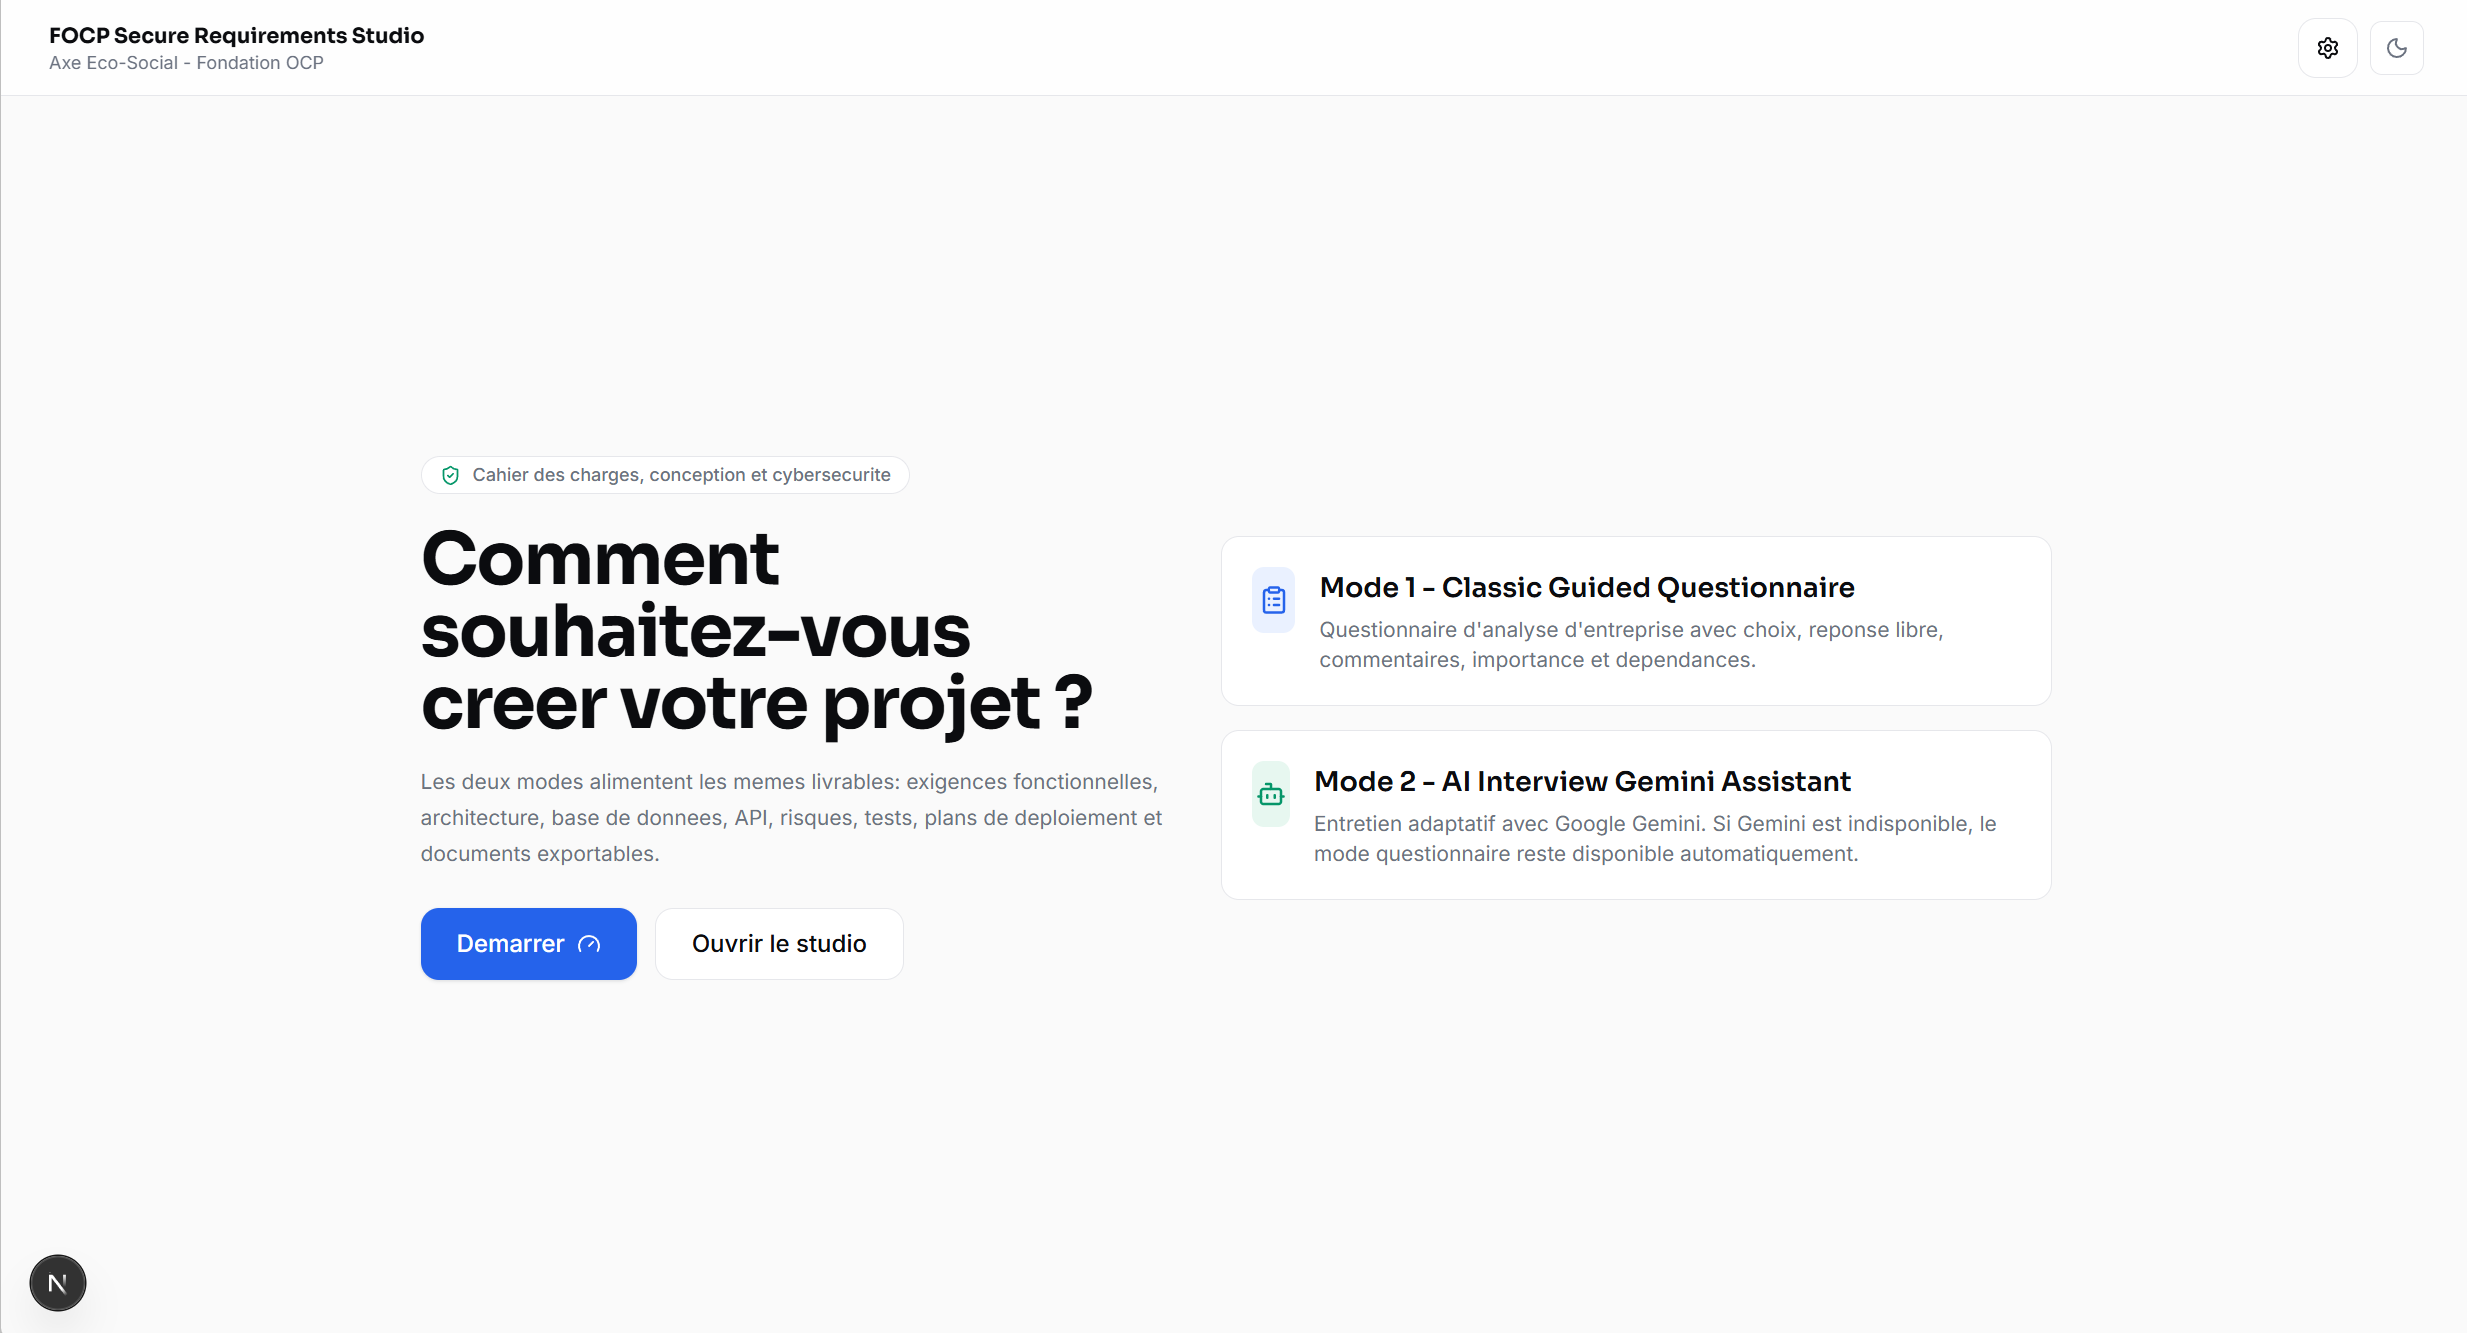
\includegraphics[width=0.92\textwidth]{figures/screenshots/srs/01_srs_accueil_mode.png}
\caption{Interface d'accueil et sélection du mode d'élicitation de projet}
\label{fig:srs_01_accueil}
\end{figure}

Cette vue permet de lancer un nouveau projet ou de charger un projet existant tout en rappelant le contexte institutionnel de la Fondation OCP.

\subsection{Formulaire d'initialisation d'un nouveau projet}

L'interface de création (figure \ref{fig:srs_02_projet}) permet de renseigner les métadonnées administratives essentielles : nom complet du projet, sigle court, direction commanditaire (Axe Social et Solidaire / DTD) et description générale du périmètre.

\begin{figure}[H]
\centering
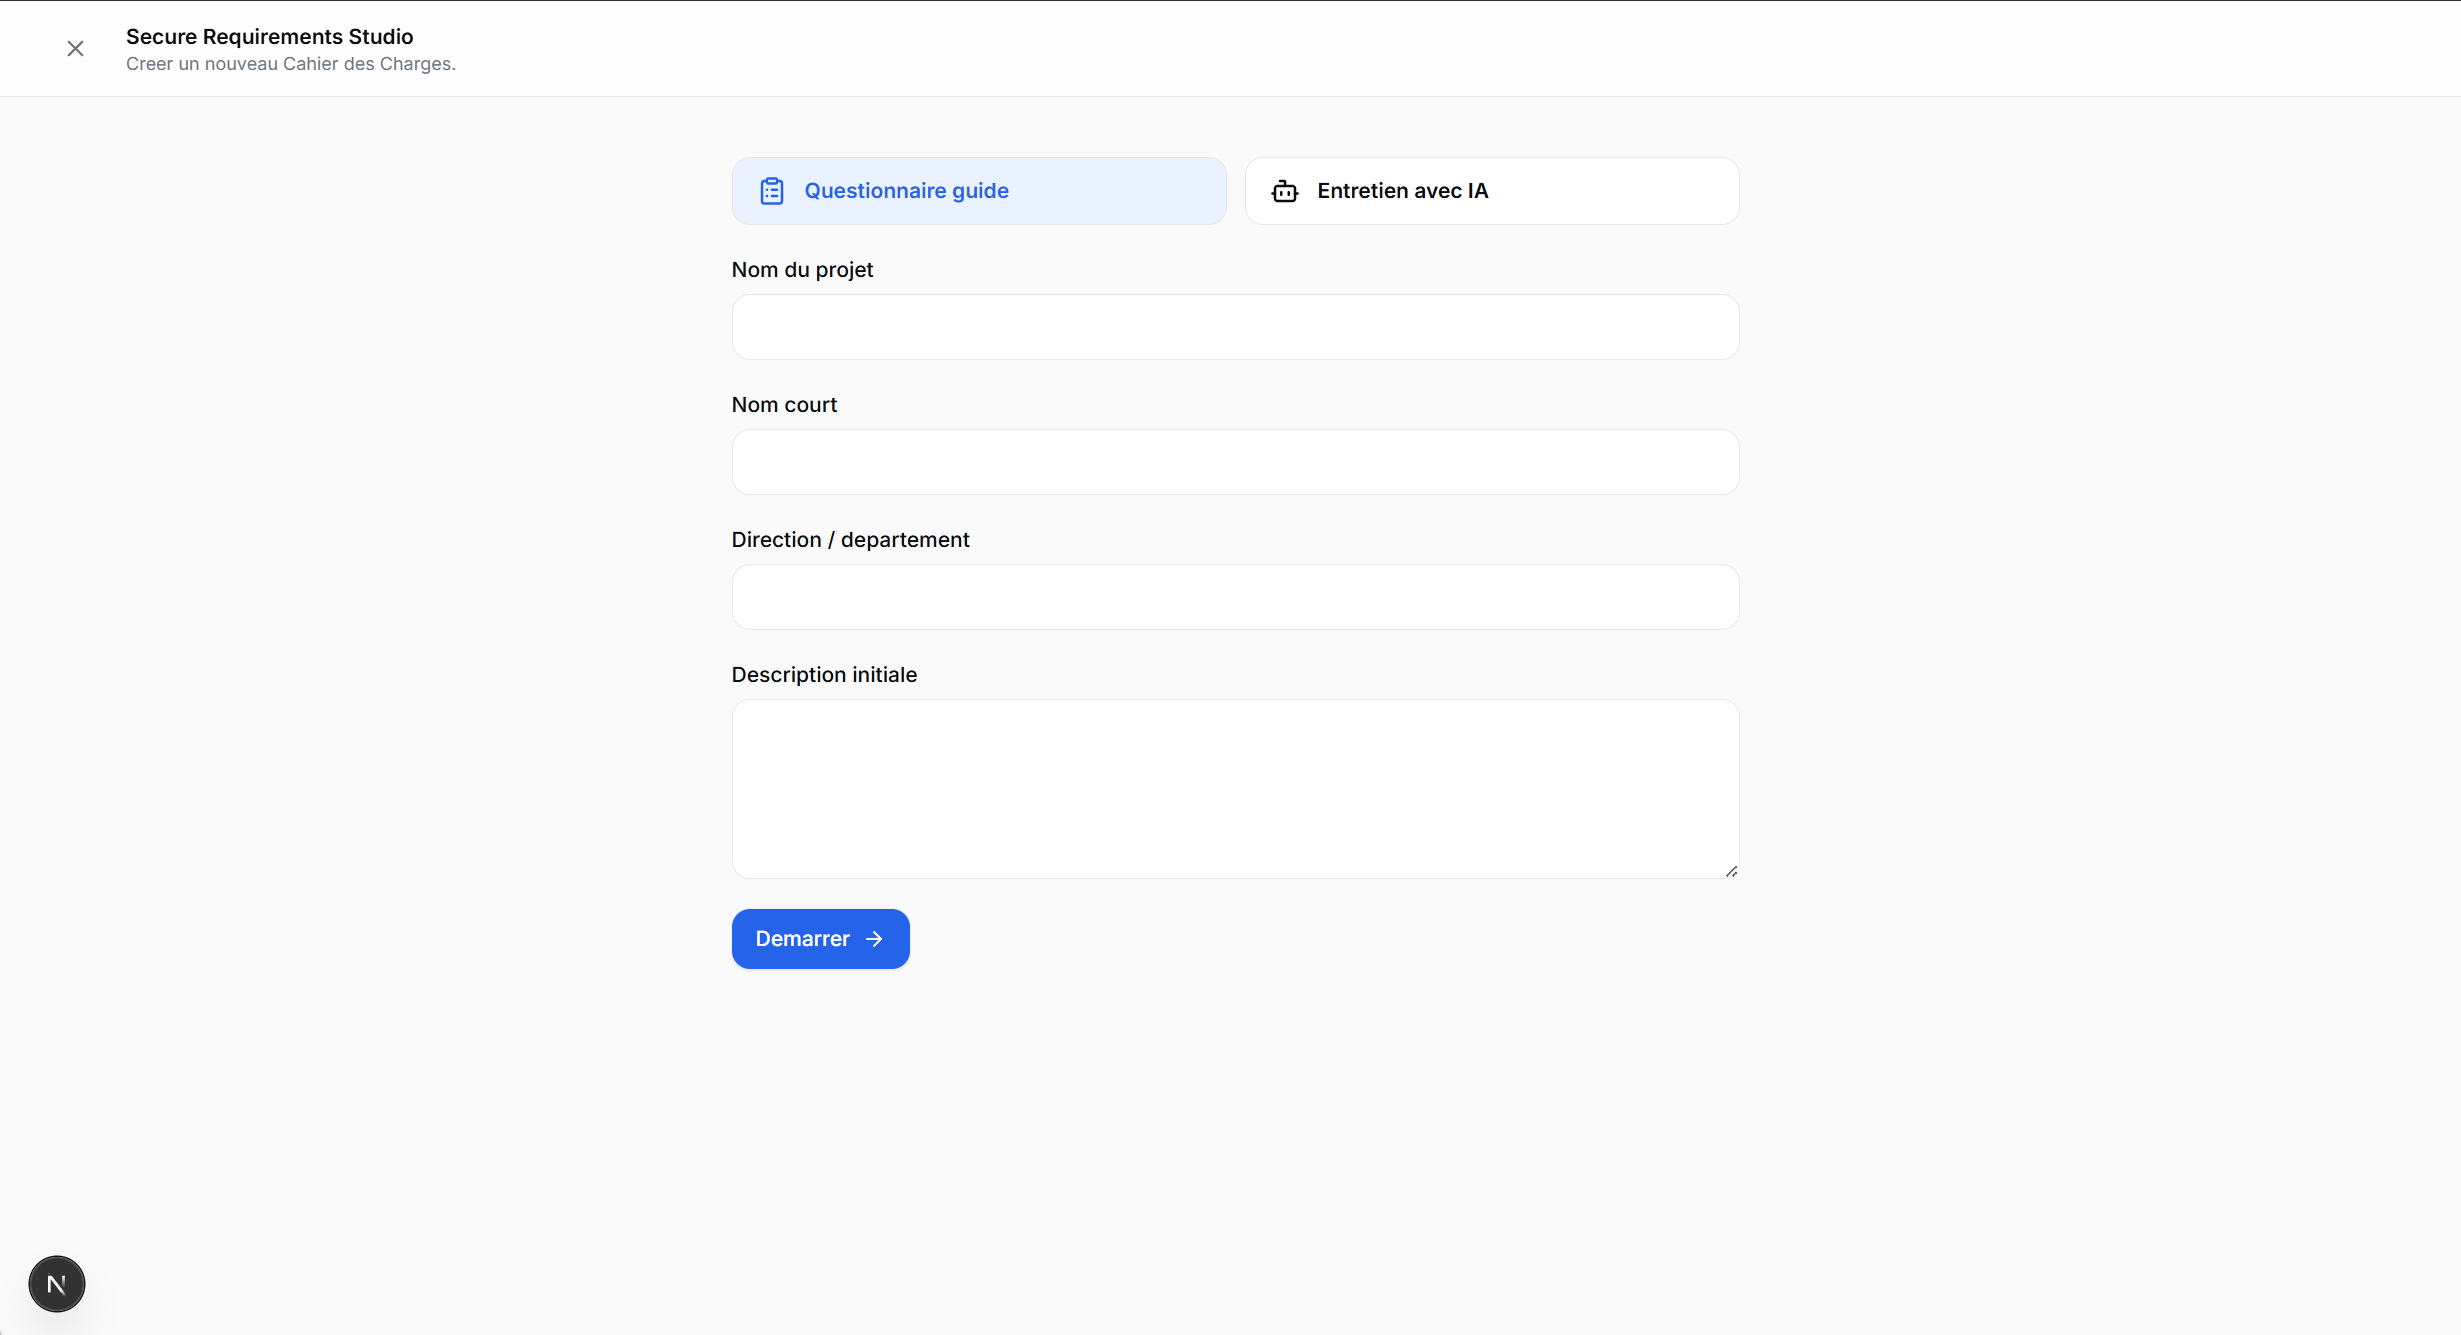
\includegraphics[width=0.92\textwidth]{figures/screenshots/srs/02_srs_nouveau_projet.png}
\caption{Formulaire d'initialisation et de paramétrage d'un nouveau projet}
\label{fig:srs_02_projet}
\end{figure}

La validation de ce formulaire instancie automatiquement en base de données le graphe de connaissances ontologique initialisé avec ses 39 concepts clés.

\subsection{Tableau de bord principal de pilotage des projets}

Le tableau de bord central (figure \ref{fig:srs_03_dashboard}) offre une vue panoramique de l'ensemble des projets de spécification initiés. Il met en avant les indicateurs de synthèse (nombre de projets, taux de complétude, score de sécurité moyen, total des exigences dérivées) ainsi que la liste détaillée des projets avec leur statut de cadrage.

\begin{figure}[H]
\centering
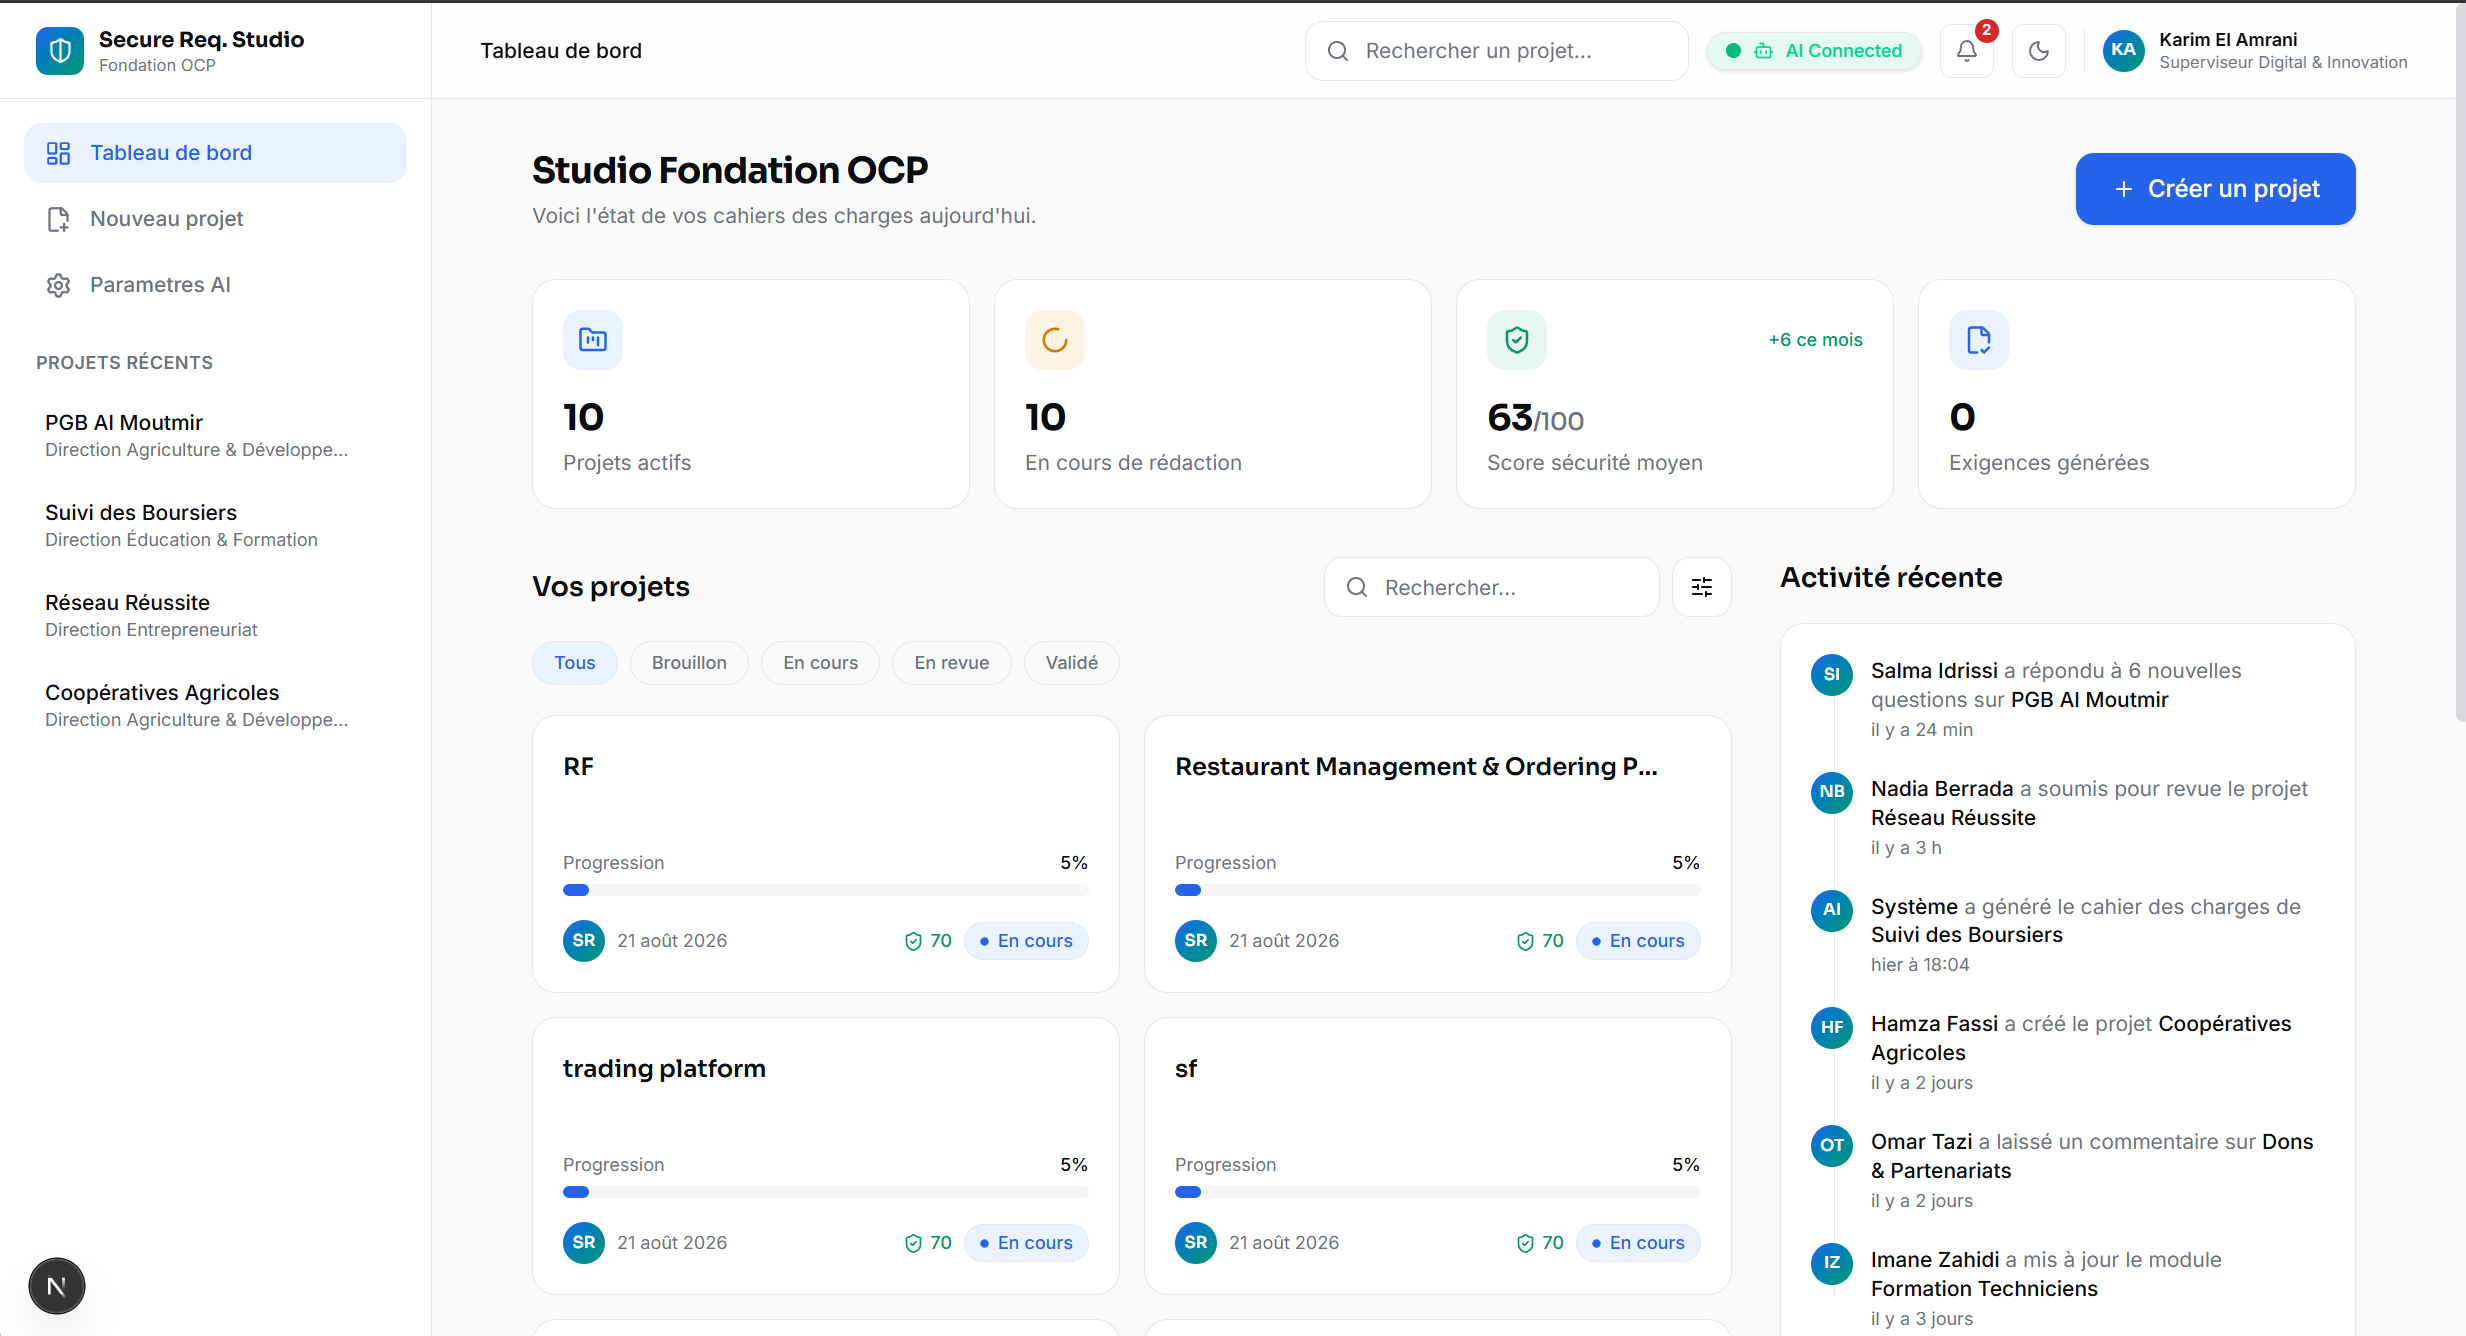
\includegraphics[width=0.92\textwidth]{figures/screenshots/srs/03_srs_dashboard.png}
\caption{Tableau de bord de supervision et de pilotage des projets de spécification}
\label{fig:srs_03_dashboard}
\end{figure}

L'analyste dispose ici d'une visibilité directe sur la maturité de chaque dossier et peut accéder aux actions de reprise d'interview, d'audit ou d'exportation.

\subsection{Paramètres et configuration des fournisseurs d'intelligence artificielle}

L'interface des paramètres (figure \ref{fig:srs_04_params}) permet de configurer les clés d'authentification API et de sélectionner le modèle de langage actif (Google Gemini 1.5 Pro ou Gemini 1.5 Flash).

\begin{figure}[H]
\centering
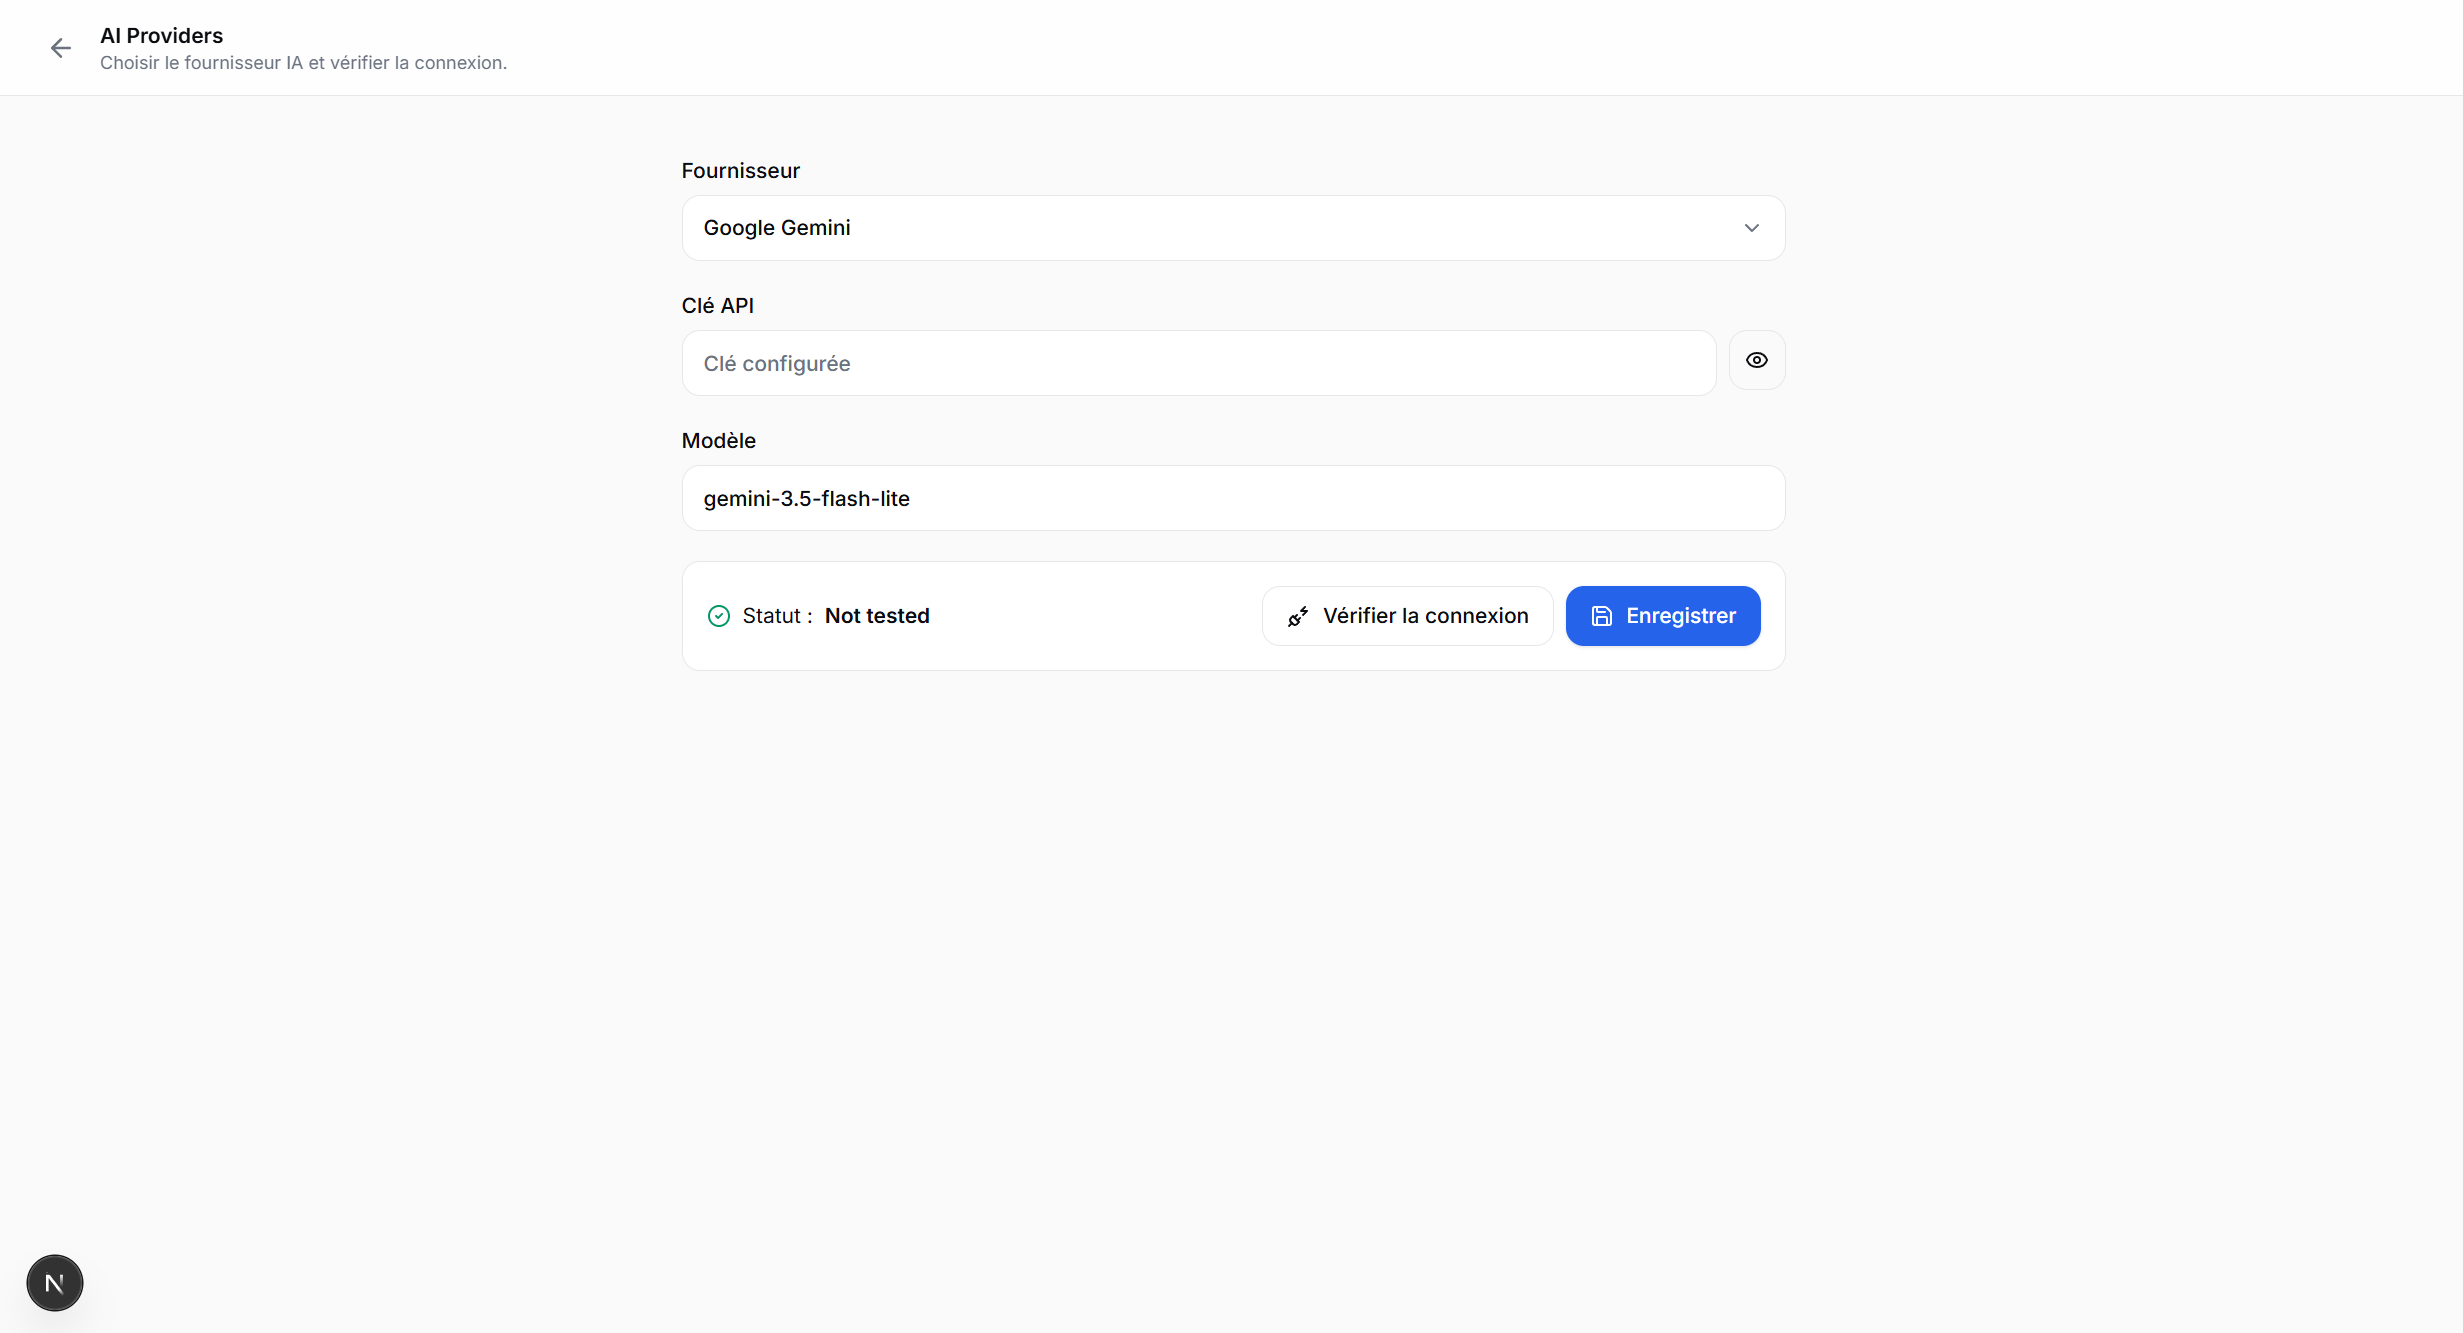
\includegraphics[width=0.92\textwidth]{figures/screenshots/srs/04_srs_parametres_ia.png}
\caption{Interface de configuration des fournisseurs d'IA et clés d'API (Google Gemini)}
\label{fig:srs_04_params}
\end{figure}

Ce paramétrage assure la flexibilité du système et garantit le basculement transparent vers le moteur déterministe local en cas de non-renseignement de clé d'API.

\subsection{Questionnaire guidé par étapes d'élicitation}

Le module d'interview guidée (figure \ref{fig:srs_05_questionnaire}) structure la capture des besoins selon une progression séquentielle par domaines : Contexte global, Utilisateurs \& Rôles, Fonctions métier, Processus \& Workflows, Contraintes techniques, Sécurité \& Priorités.

\begin{figure}[H]
\centering
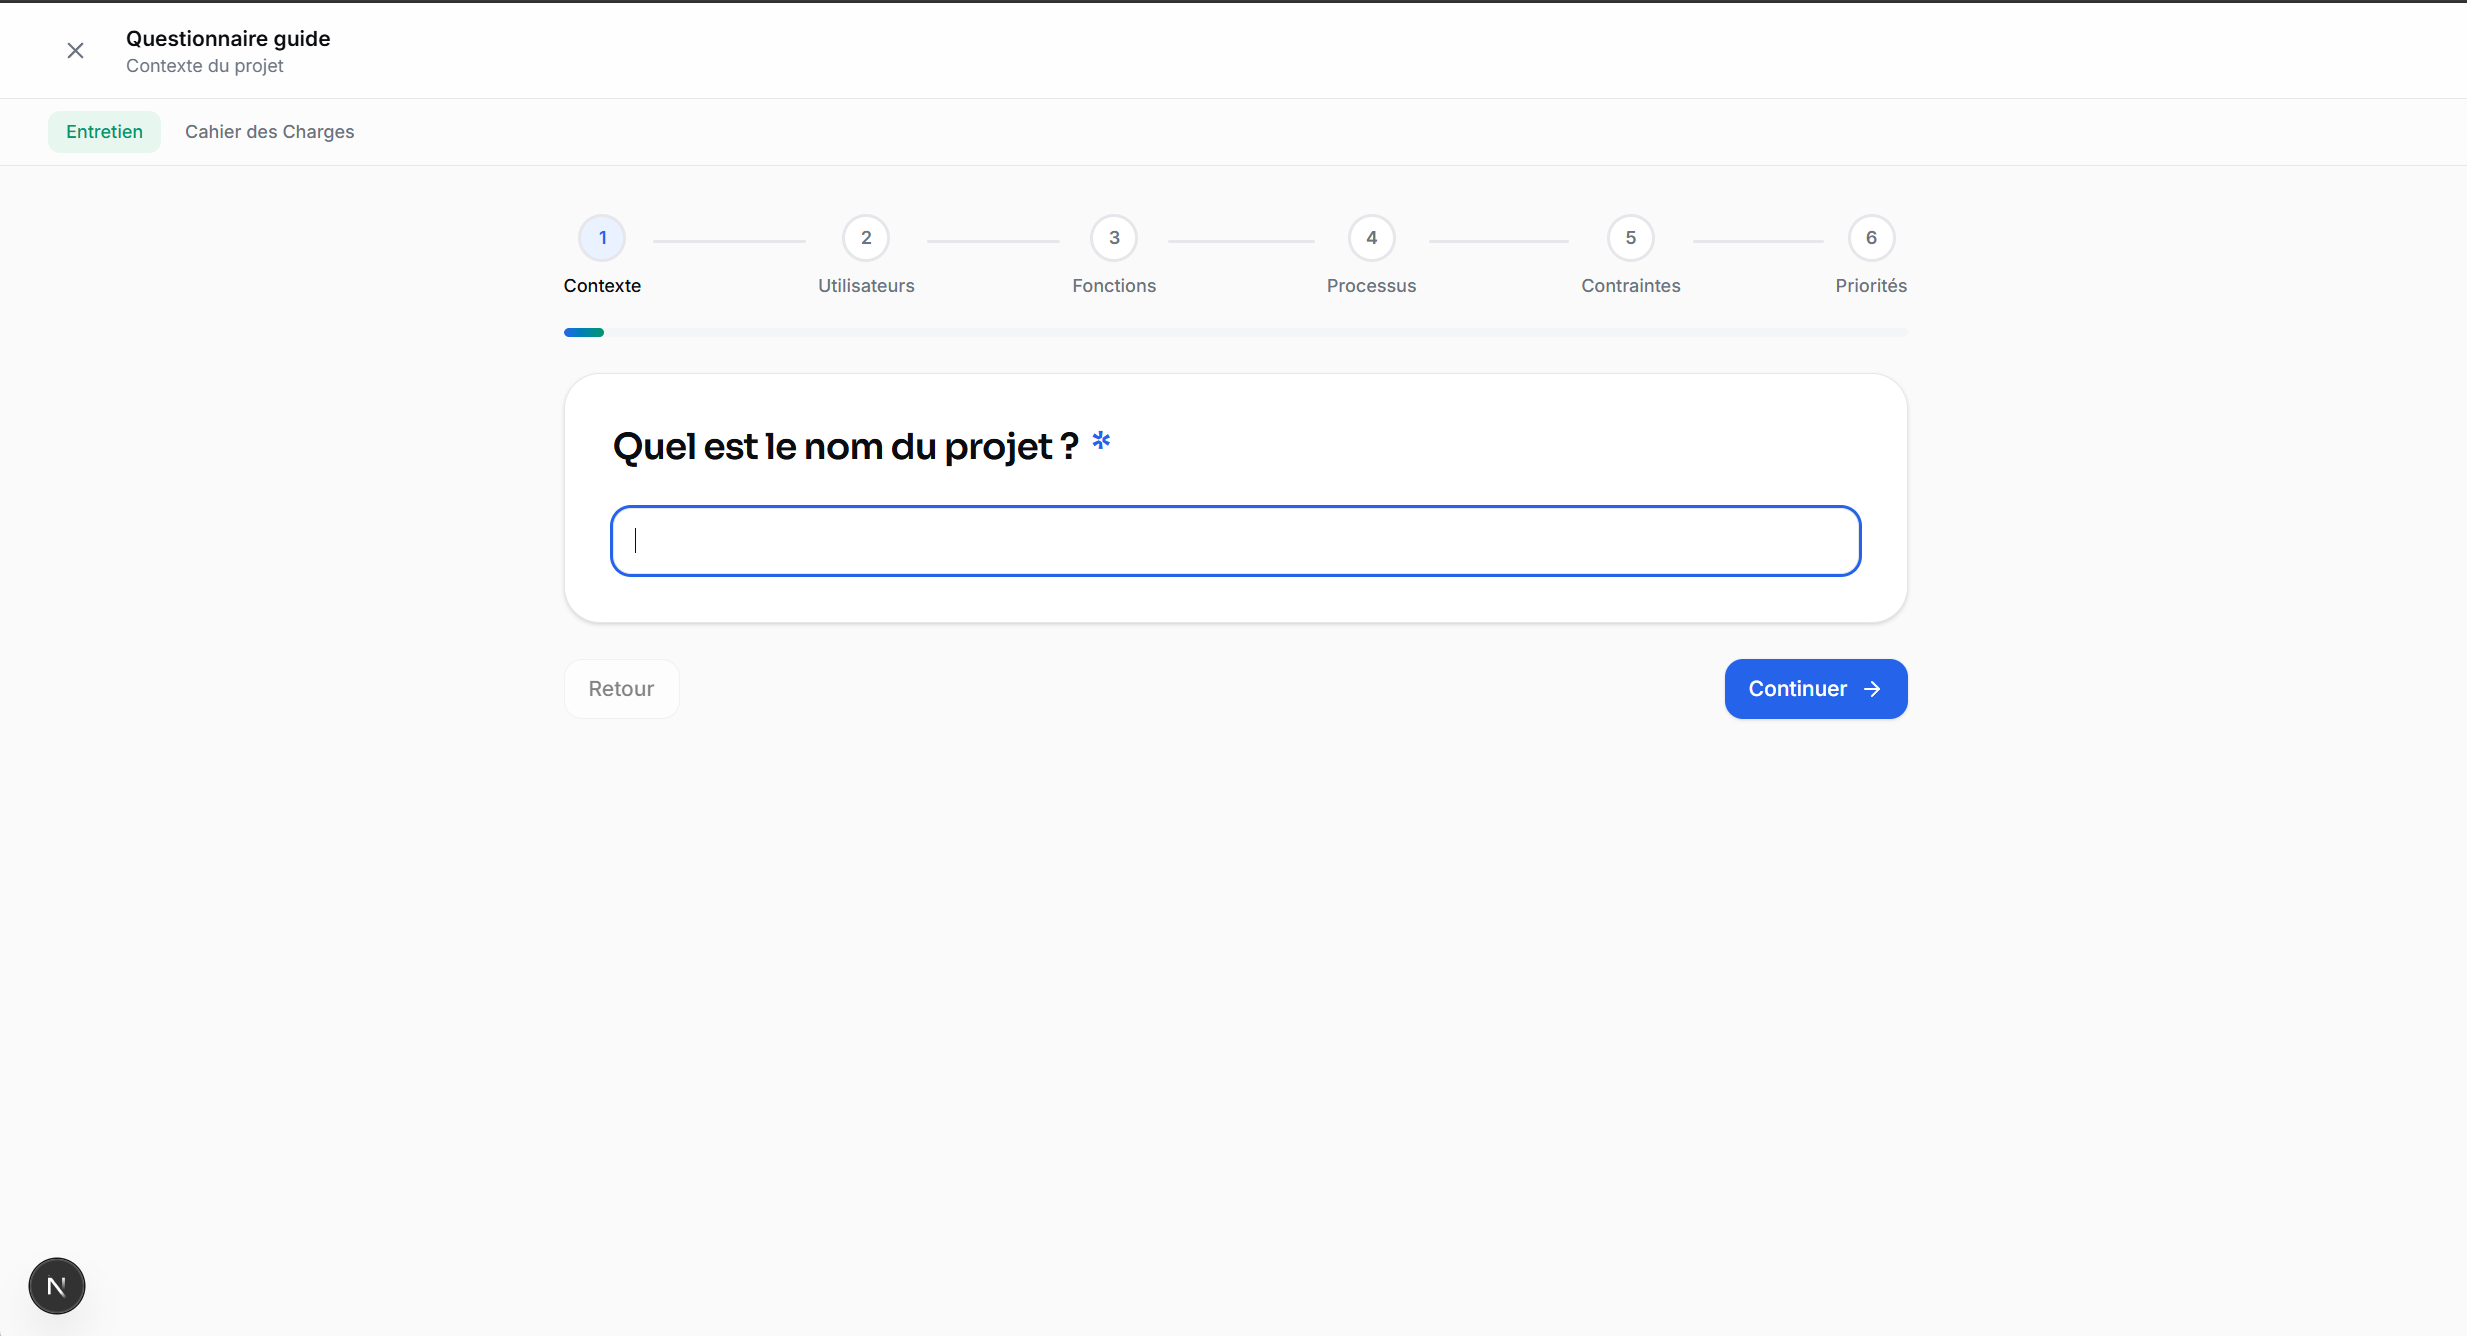
\includegraphics[width=0.92\textwidth]{figures/screenshots/srs/05_srs_questionnaire_guide.png}
\caption{Interface du questionnaire d'élicitation structuré par étapes thématiques}
\label{fig:srs_05_questionnaire}
\end{figure}

Chaque réponse validée par l'analyste déclenche une mise à jour instantanée du graphe conceptuel et la dérivation dynamique des exigences fonctionnelles et de sécurité associées.

\subsection{Prévisualisation du Cahier des Charges généré}

L'interface de prévisualisation (figure \ref{fig:srs_06_preview}) permet de visualiser en direct la structure complète du document de spécification assemblé par le moteur documentaire.

\begin{figure}[H]
\centering
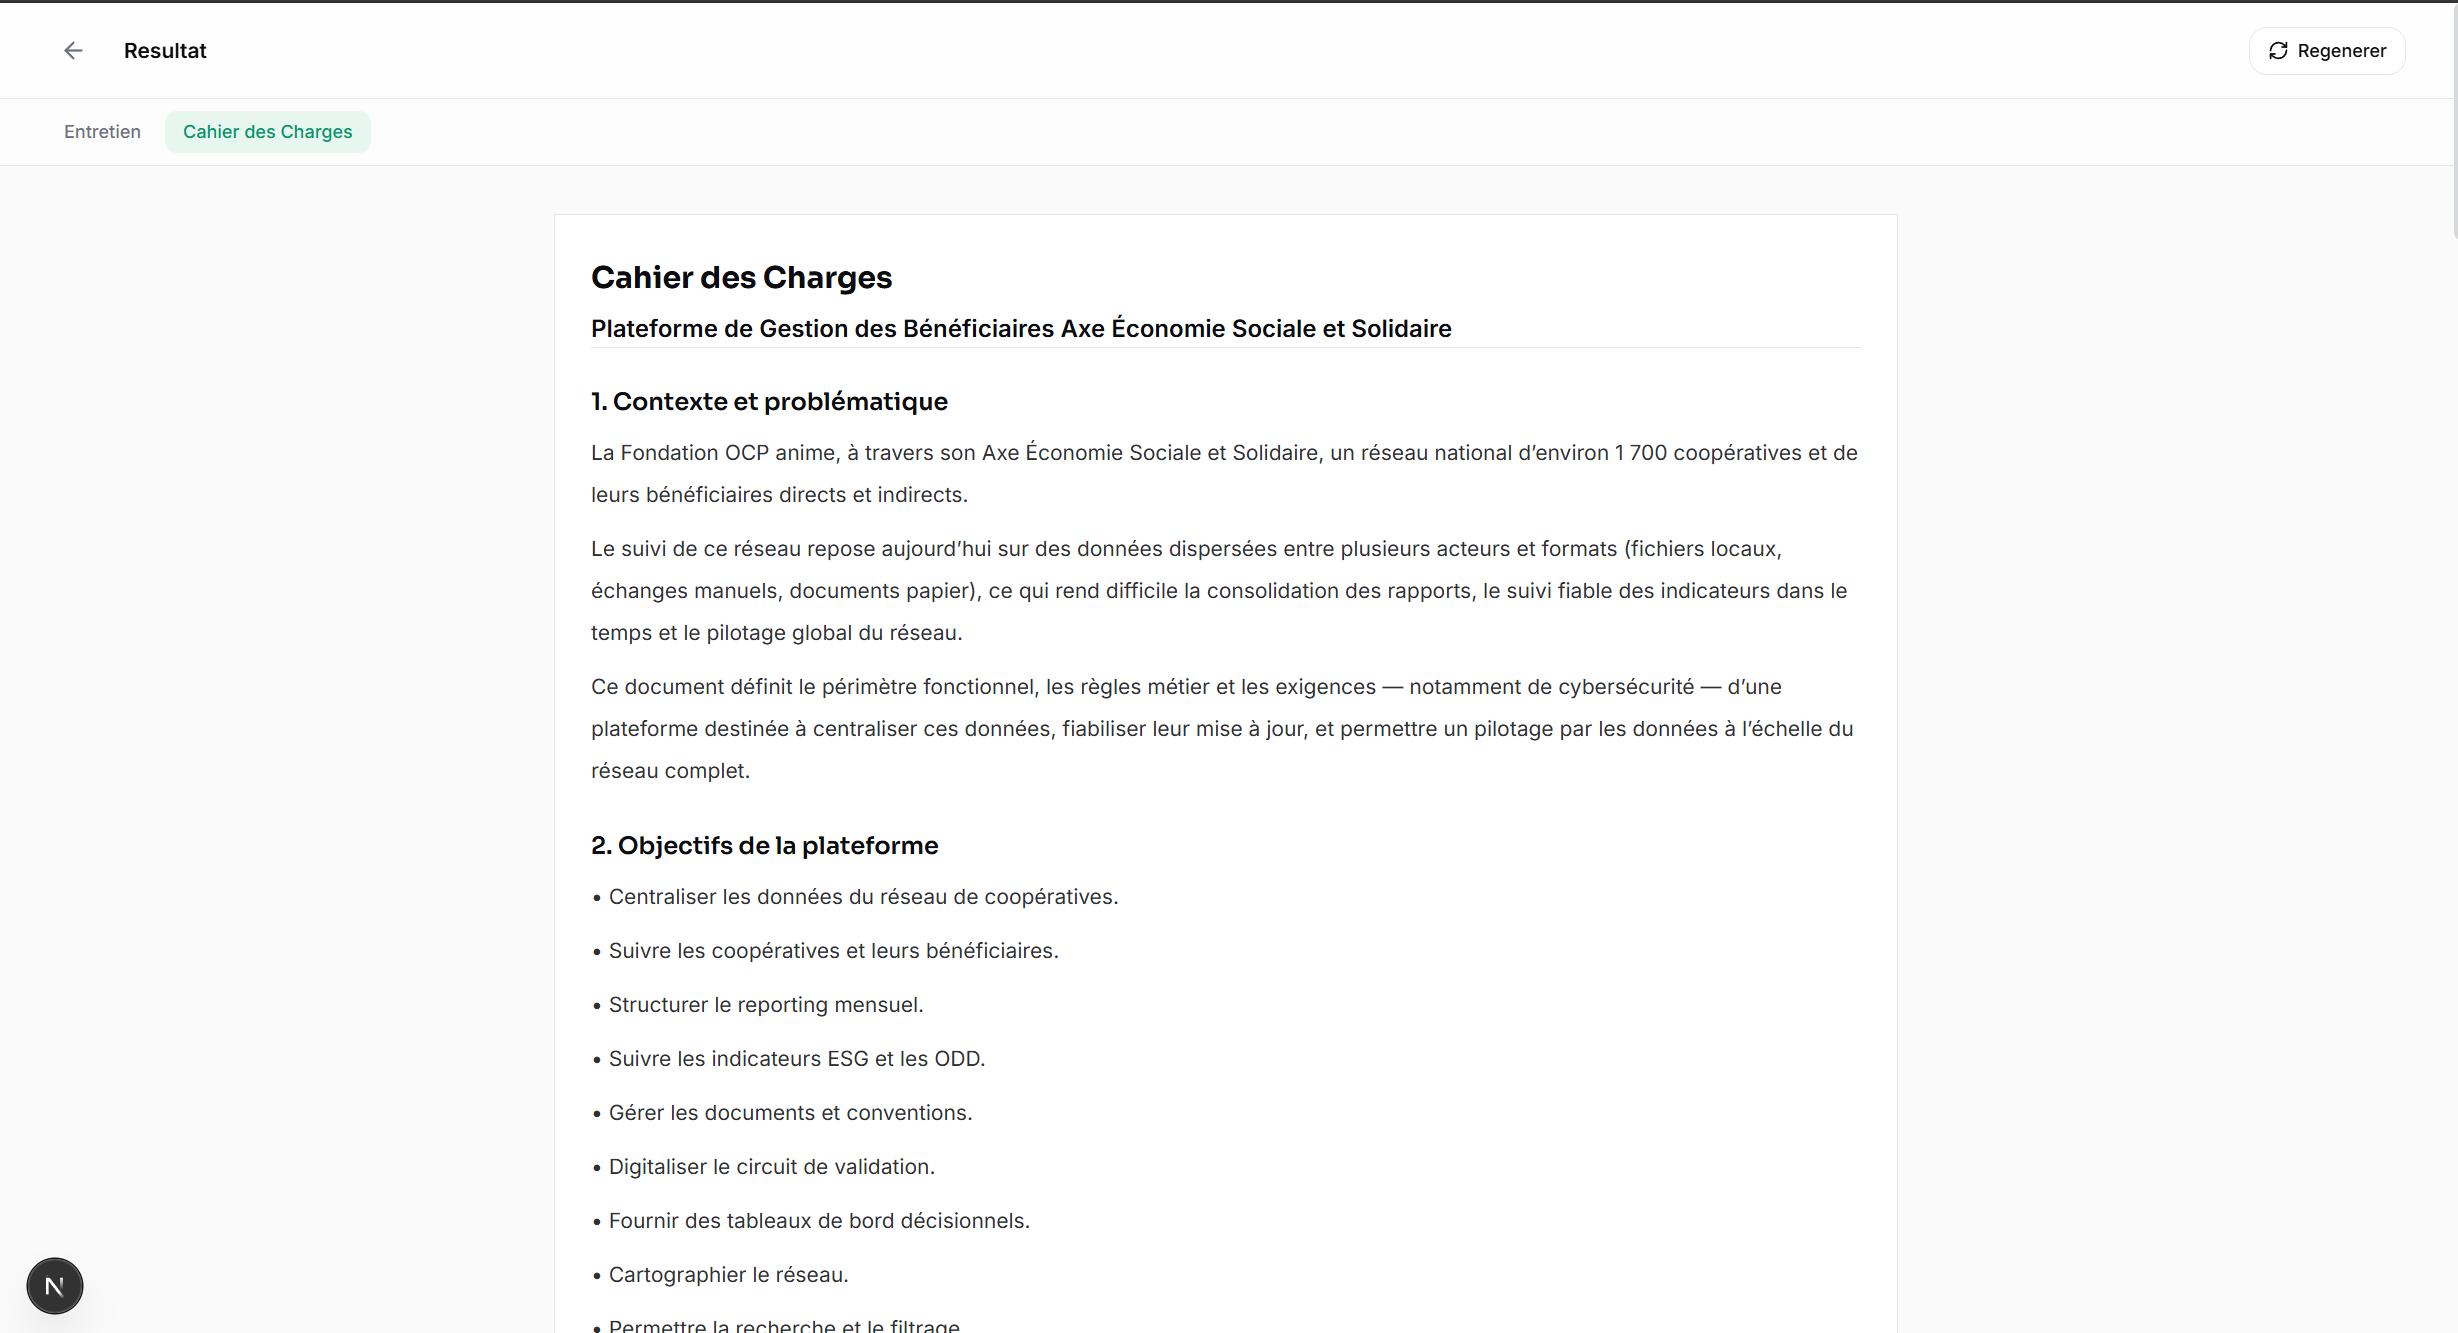
\includegraphics[width=0.92\textwidth]{figures/screenshots/srs/06_srs_cahier_charges_preview.png}
\caption{Interface de prévisualisation interactive du Cahier des Charges assemblé}
\label{fig:srs_06_preview}
\end{figure}

L'utilisateur y vérifie l'articulation entre les objectifs stratégiques, les profils d'utilisateurs RBAC, les entités manipulées et les critères d'acceptation avant d'engager le téléchargement dans le format de son choix (PDF, DOCX, Markdown, LaTeX).

\subsection{Résumé et analyse de maturité du projet}

L'interface de synthèse (figure \ref{fig:srs_07_resume}) dresse le bilan d'évaluation du projet : état d'homologation, score de cybersécurité calculé, modules fonctionnels détectés et rôles identifiés.

\begin{figure}[H]
\centering
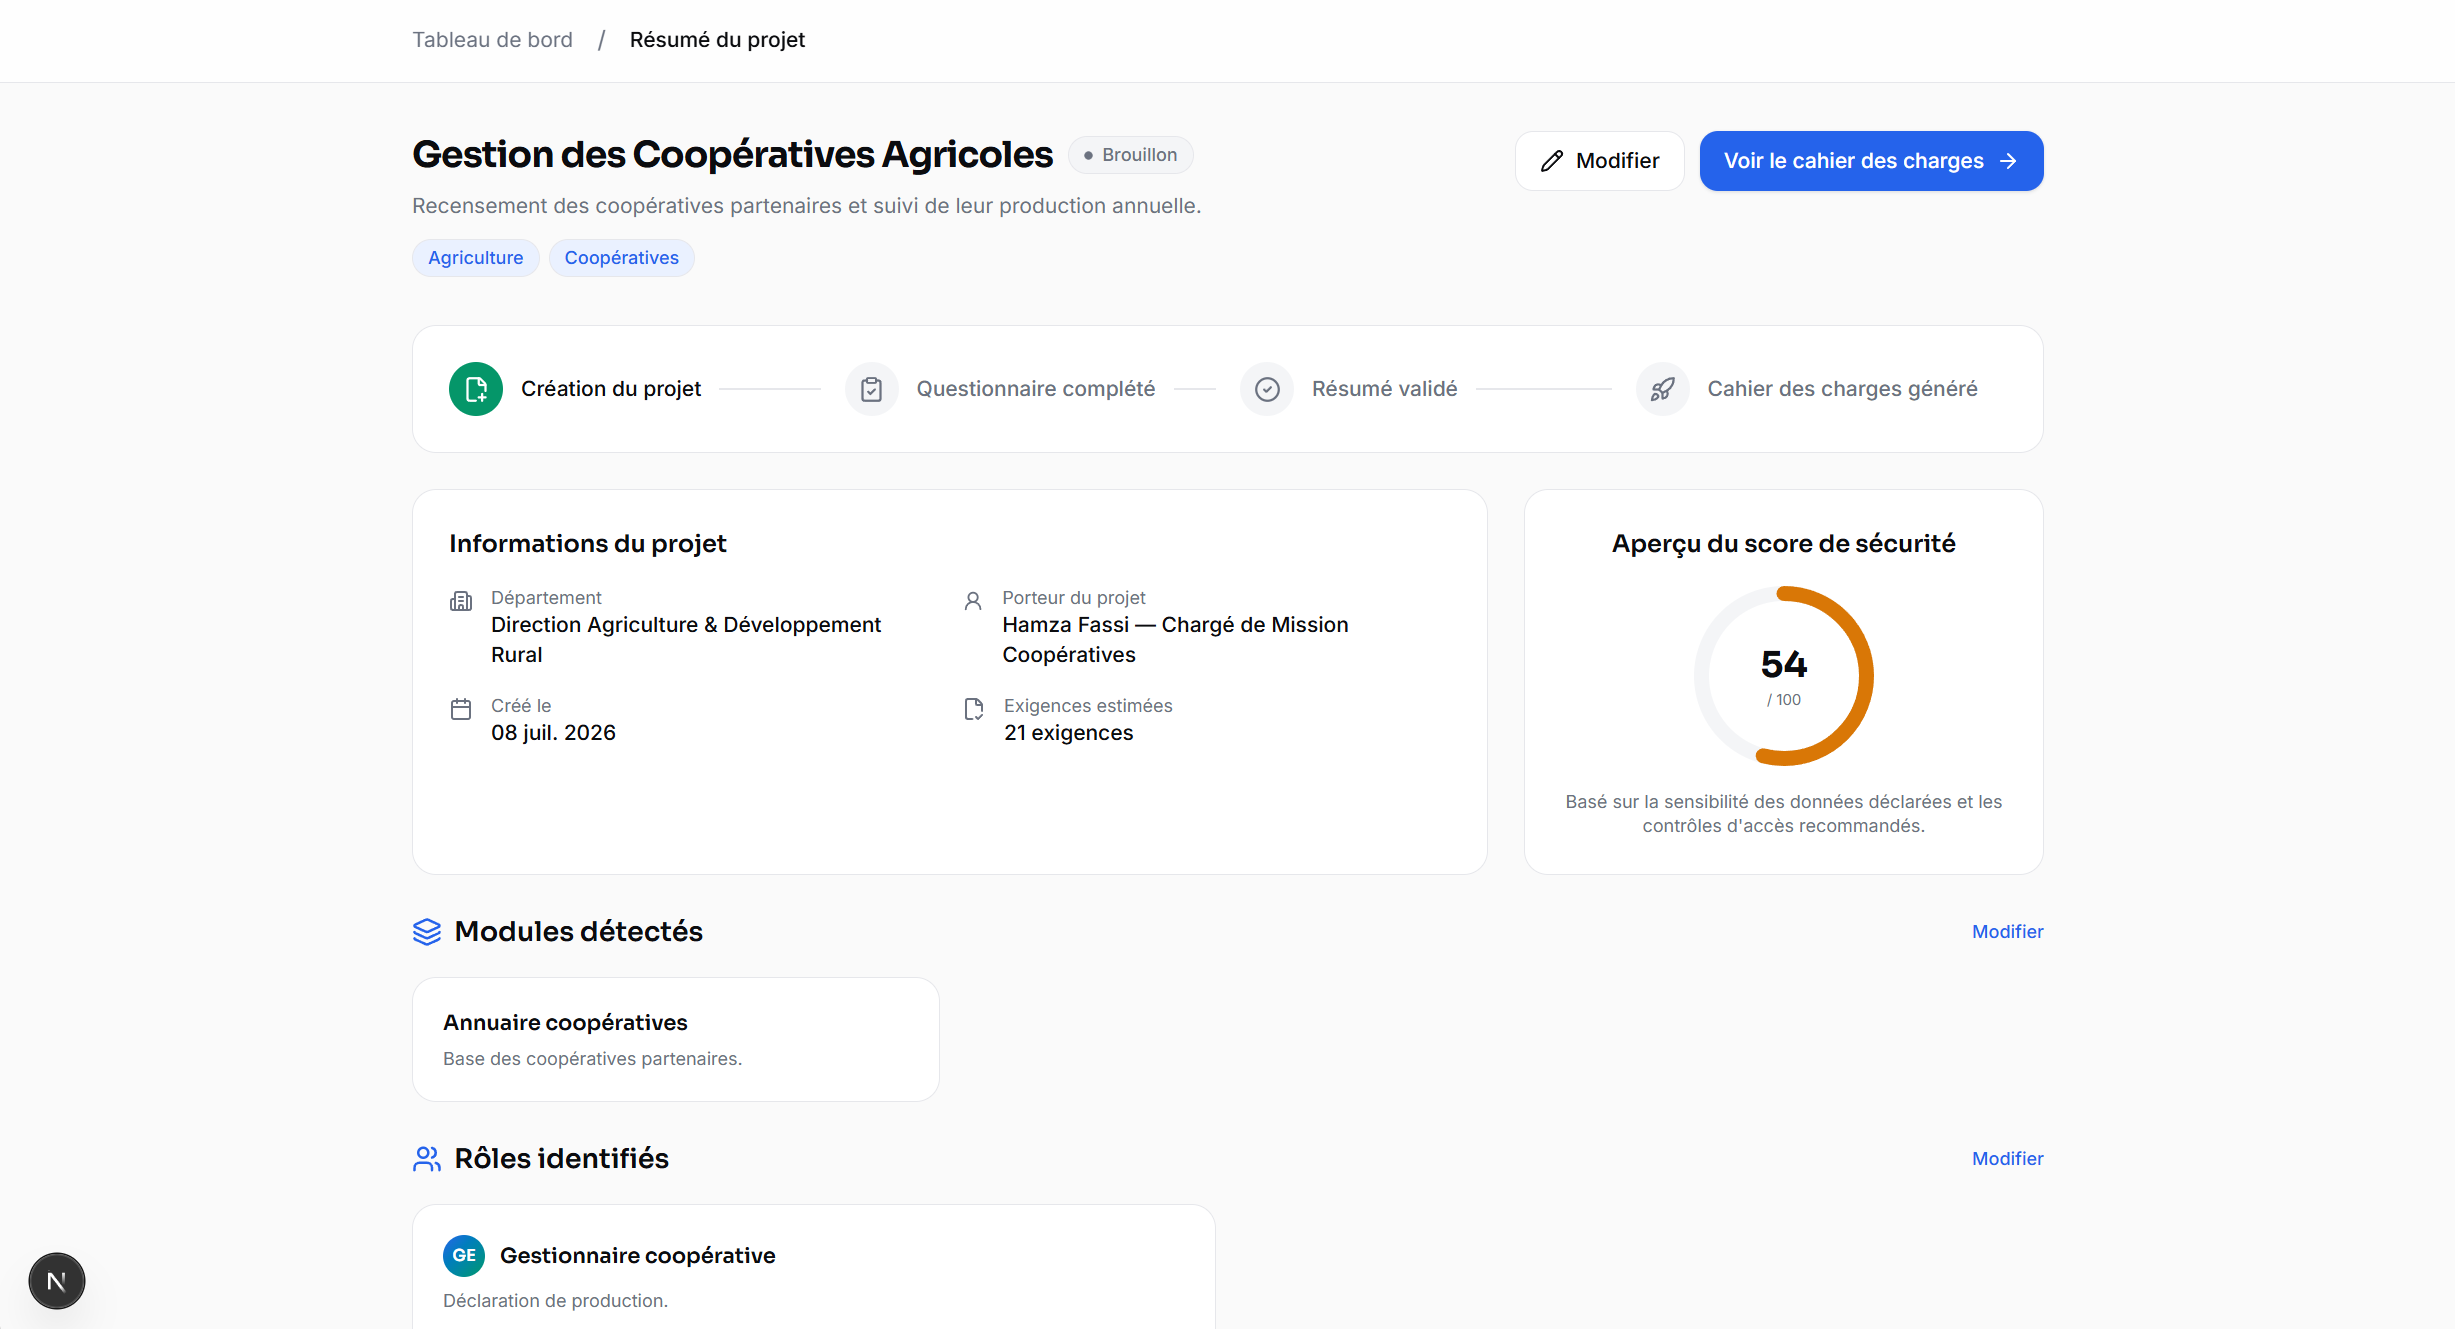
\includegraphics[width=0.92\textwidth]{figures/screenshots/srs/07_srs_resume_projet.png}
\caption{Interface de synthèse du projet : statut, score de sécurité et modules détectés}
\label{fig:srs_07_resume}
\end{figure}

Cette vue fournit une traçabilité complète permettant d'attester que le dossier de spécification a atteint le niveau de qualité requis pour engager la phase de réalisation.

\section[Analyse du livrable final : Cahier des Charges FOCP V3]{Analyse du livrable final~: {\ttfamily Cahier\allowbreak\_\allowbreak des\allowbreak\_\allowbreak Charges\allowbreak\_\allowbreak FOCP\allowbreak\_\allowbreak V3.pdf}}

L'aboutissement opérationnel direct de notre application logicielle SRS est la production du document officiel de référence : {\ttfamily Cahier\allowbreak\_\allowbreak des\allowbreak\_\allowbreak Charges\allowbreak\_\allowbreak FOCP\allowbreak\_\allowbreak V3.pdf}.

Ce livrable formalise l'intégralité des spécifications de la future \textbf{plateforme de gestion des bénéficiaires de l'Axe Social et Solidaire au sein de la Fondation OCP en intégrant des exigences de cybersécurité}. L'analyse de sa structure révèle les sections majeures générées automatiquement par notre système :
\begin{enumerate}
    \item \textbf{Contexte et problématique} : Définition du réseau de 1\,700 coopératives et justification du besoin de centralisation et de sécurisation des données.
    \item \textbf{Objectifs de la plateforme} : 12 objectifs stratégiques (centralisation, reporting mensuel, indicateurs ESG/ODD, gestion documentaire, cartographie, traçabilité, cybersécurité).
    \item \textbf{Utilisateurs et permissions (RBAC)} : Définition stricte des rôles \textit{Administrateur Fondation OCP} (accès global, analyse, validation, correction exceptionnelle tracée) et \textit{Représentant de coopérative} (accès limité à son profil, déclaration des bénéficiaires et activités).
    \item \textbf{Données gérées} : Structuration des données des coopératives, bénéficiaires directs et indirects (femmes, jeunes, handicap, agriculteurs), activités, documents et conventions.
    \item \textbf{Workflow mensuel de soumission et validation} : Circuit digitalisé de saisie, soumission, validation ou rejet motivé avec notification et correction traçable.
    \item \textbf{Tableaux de bord et cartographie} : Spécification des KPI décisionnels et de la carte interactive géolocalisant les coopératives par région et province.
    \item \textbf{Exigences de cybersécurité transversales} : Contrôle d'accès RBAC, principe du moindre privilège, politique de mot de passe, chiffrement des données sensibles, validation des fichiers et journalisation systématique de toutes les opérations.
    \item \textbf{Critères d'acceptation et de validation} : Liste des critères d'homologation et points de décision soumis à arbitrage avec la Fondation.
\end{enumerate}

Ce livrable démontre la capacité de notre application logicielle SRS à transformer un processus d'élicitation complexe en un document de spécification hautement qualifié, rigoureux et prêt à l'emploi.

\section{Conclusion}

Ce chapitre a illustré la réalisation logicielle effective de l'application \textbf{Secure Requirements Studio (SRS)}. L'écosystème technologique moderne (FastAPI, Next.js 15, SQLAlchemy, Docker, Google Gemini) a permis d'implémenter avec succès les modules de capture ontologique, d'analyse de cybersécurité, d'audit qualité et d'assemblage documentaire. Cette chaîne a permis de produire le document officiel {\ttfamily Cahier\allowbreak\_\allowbreak des\allowbreak\_\allowbreak Charges\allowbreak\_\allowbreak FOCP\allowbreak\_\allowbreak V3.pdf}.

Afin de concrétiser ces spécifications et d'en valider l'opérabilité par une preuve de concept concrète, nous avons développé le prototype fonctionnel (MVP) de la plateforme de gestion des bénéficiaires, dont la réalisation et les interfaces détaillées font l'objet du chapitre 5 suivant.

\newpage

\chapter{Réalisation et présentation du MVP de la plateforme des bénéficiaires}
\markboth{CHAPITRE 5. RÉALISATION DU MVP DE LA PLATEFORME}{CHAPITRE 5. RÉALISATION DU MVP DE LA PLATEFORME}

\section{Introduction}

La formalisation du document de référence {\ttfamily Cahier\allowbreak\_\allowbreak des\allowbreak\_\allowbreak Charges\allowbreak\_\allowbreak FOCP\allowbreak\_\allowbreak V3.pdf} par l'application Secure Requirements Studio (SRS) a permis d'établir avec une grande précision l'ensemble des spécifications fonctionnelles, techniques et de cybersécurité de la future plateforme cible de la Fondation OCP. Afin de concrétiser cette démarche d'ingénierie et d'apporter une preuve de concept opérationnelle, nous avons développé le \textbf{MVP (Minimum Viable Product)} de la \textbf{plateforme de gestion des bénéficiaires de l'Axe Social et Solidaire}.

Ce cinquième chapitre est dédié à la présentation détaillée de ce prototype fonctionnel. Nous y exposons les objectifs et le périmètre retenus pour le MVP, décrivons son architecture fonctionnelle modulaire, détaillons l'ensemble de ses interfaces graphiques réelles, et analysons la matrice de conformité et de traçabilité attestant de la parfaite adéquation entre le Cahier des Charges généré et le démonstrateur réalisé.

\section{Objectifs et périmètre du MVP}

Le MVP a été conçu comme une implémentation de référence hautement représentative des processus métier de l'Axe Social et Solidaire. Il vise les objectifs opérationnels suivants :

\begin{itemize}
    \item \textbf{Démontrer la faisabilité technique} de la centralisation des données pour un réseau national de 1\,700 coopératives réparties sur les douze régions du Royaume.
    \item \textbf{Valider le contrôle d'accès basé sur les rôles (RBAC)} en instanciant les espaces différenciés pour les Administrateurs Fondation OCP et les Représentants de coopératives.
    \item \textbf{Dématérialiser le workflow mensuel de reporting} comprenant la saisie des bénéficiaires (directs et indirects), le calcul des parités, la soumission et les actions de validation ou de rejet motivé.
    \item \textbf{Offrir une visualisation géographique interactive} facilitant le repérage spatial des coopératives et l'analyse territoriale des actions de la Fondation.
    \item \textbf{Piloter les indicateurs d'impact durable} par la consolidation automatisée des métriques ESG et des Objectifs de Développement Durable (ODD).
\end{itemize}

\section{Architecture fonctionnelle du MVP}

L'architecture du MVP s'articule autour de modules interconnectés garantissant la modularité, la sécurité et la fluidité des traitements :

\begin{enumerate}
    \item \textbf{Module d'Authentification et Sécurité RBAC} : Gestion des sessions sécurisées, contrôle strict des privilèges et traçabilité des connexions.
    \item \textbf{Module Tableau de Bord Décisionnel} : Agrégation temps réel des KPI d'impact, distribution par genre et suivi de l'évolution mensuelle.
    \item \textbf{Module Annuaire des Coopératives} : Fiches détaillées, contacts, statut juridique, filière d'activité et gouvernance.
    \item \textbf{Module Cartographie Interactive (SIG)} : Visualisation cartographique dynamique avec regroupement par clusters et filtres multicritères.
    \item \textbf{Module Déclarations \& Rapports Mensuels} : Saisie structurée, calcul automatique des bénéficiaires et circuit de validation avec historique.
    \item \textbf{Module Conventions \& Gestion Budgétaire} : Suivi des engagements contractuels, taux de consommation budgétaire et échéanciers.
    \item \textbf{Module Gestion Électronique des Documents (GED)} : Téléversement sécurisé des pièces justificatives, validation et horodatage.
    \item \textbf{Module Moteur d'Importation \& Exportation} : Traitement par lots via fichiers CSV, et génération de rapports de synthèse (Excel, PDF).
    \item \textbf{Module Centre de Notifications} : Alertes contextuelles sur les échéances de reporting et les retours de validation.
\end{enumerate}

\section{Principales interfaces graphiques du prototype MVP}

Nous présentons ci-après l'ensemble des treize interfaces développées pour le MVP de la plateforme de gestion des bénéficiaires.

\subsection{Accueil et authentification sécurisée (RBAC)}

L'écran d'accueil et d'authentification (figure \ref{fig:mvp_01_auth}) constitue le point d'entrée unique de la plateforme. Il intègre une authentification robuste permettant d'orienter l'utilisateur vers son espace dédié selon son rôle : \textit{Administrateur Fondation} ou \textit{Représentant de Coopérative}.

\begin{figure}[H]
\centering
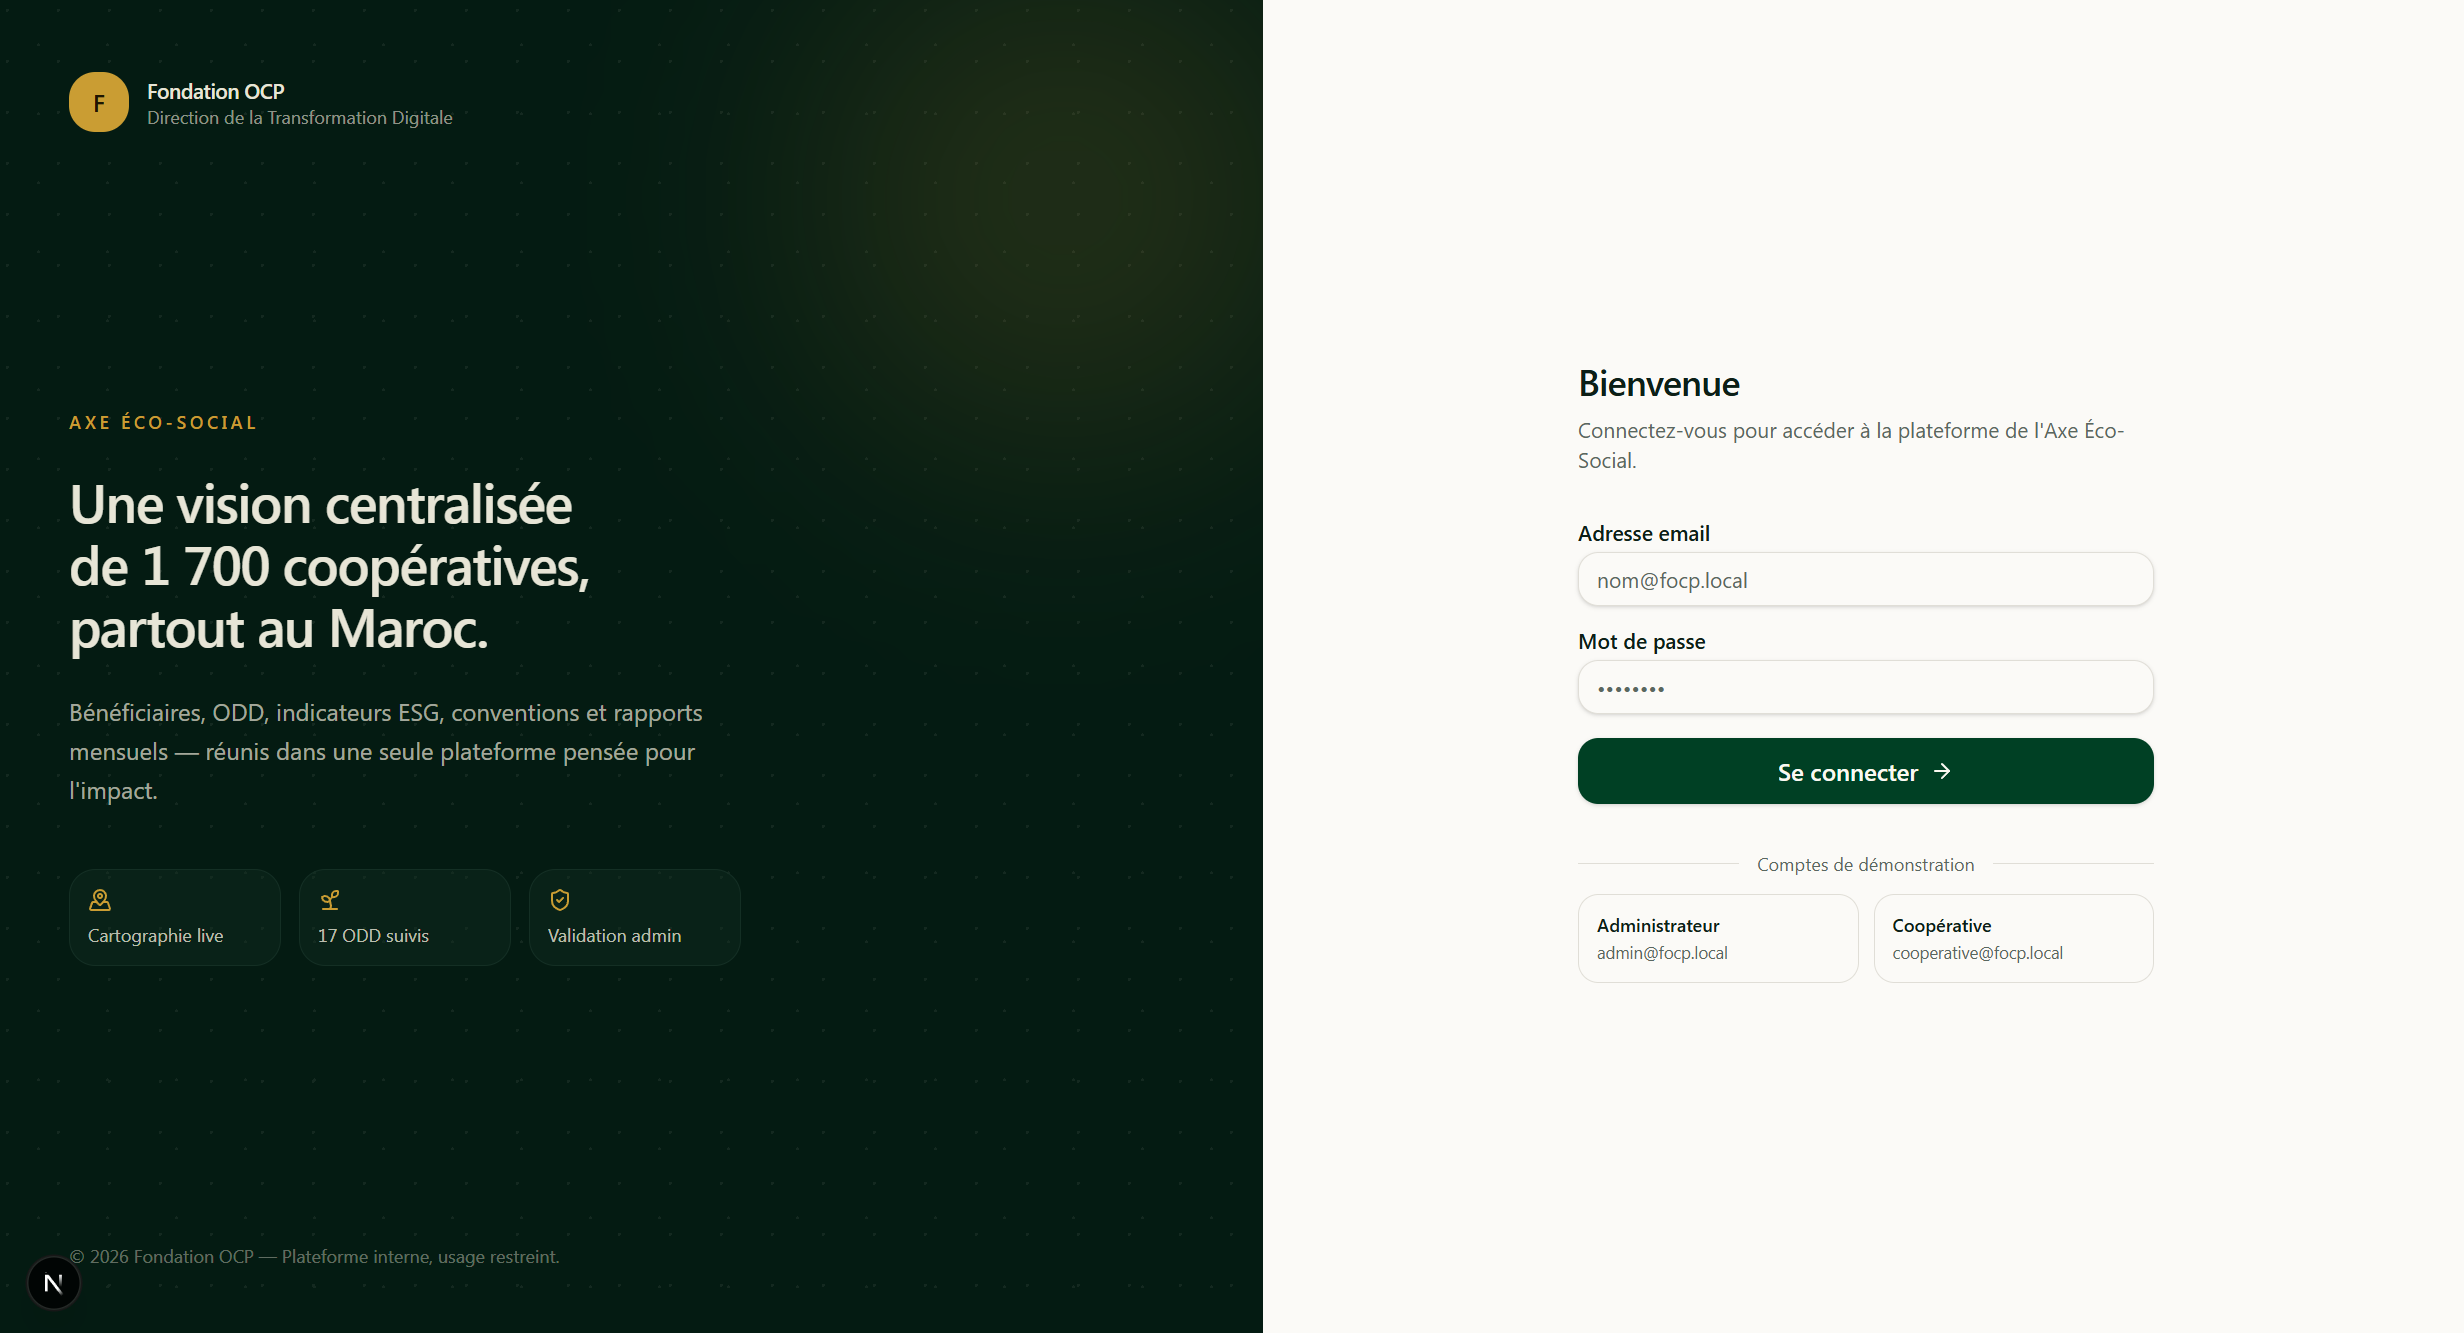
\includegraphics[width=0.90\textwidth]{figures/screenshots/mvp/01_mvp_authentification.png}
\caption{Interface d'accueil et d'authentification sécurisée (RBAC)}
\label{fig:mvp_01_auth}
\end{figure}

Cette interface assure le respect des politiques de sécurité spécifiées (mots de passe forts, protection contre les attaques par force brute et limitation de session).

\subsection{Tableau de bord général de pilotage de l'Axe Social et Solidaire}

Le tableau de bord principal (figure \ref{fig:mvp_02_dash}) offre une vue panoramique et décisionnelle sur l'ensemble du réseau national. Il affiche en temps réel :
\begin{itemize}
    \item Le nombre total de coopératives actives et de conventions signées.
    \item Le volume consolidé des bénéficiaires directs (femmes, jeunes, handicapés, agriculteurs) et indirects.
    \item La répartition des projets selon les Objectifs de Développement Durable (ODD 1, 5, 8, 10, etc.).
    \item L'évolution mensuelle des bénéficiaires et le taux de conformité des rapports déposés.
\end{itemize}

\begin{figure}[H]
\centering
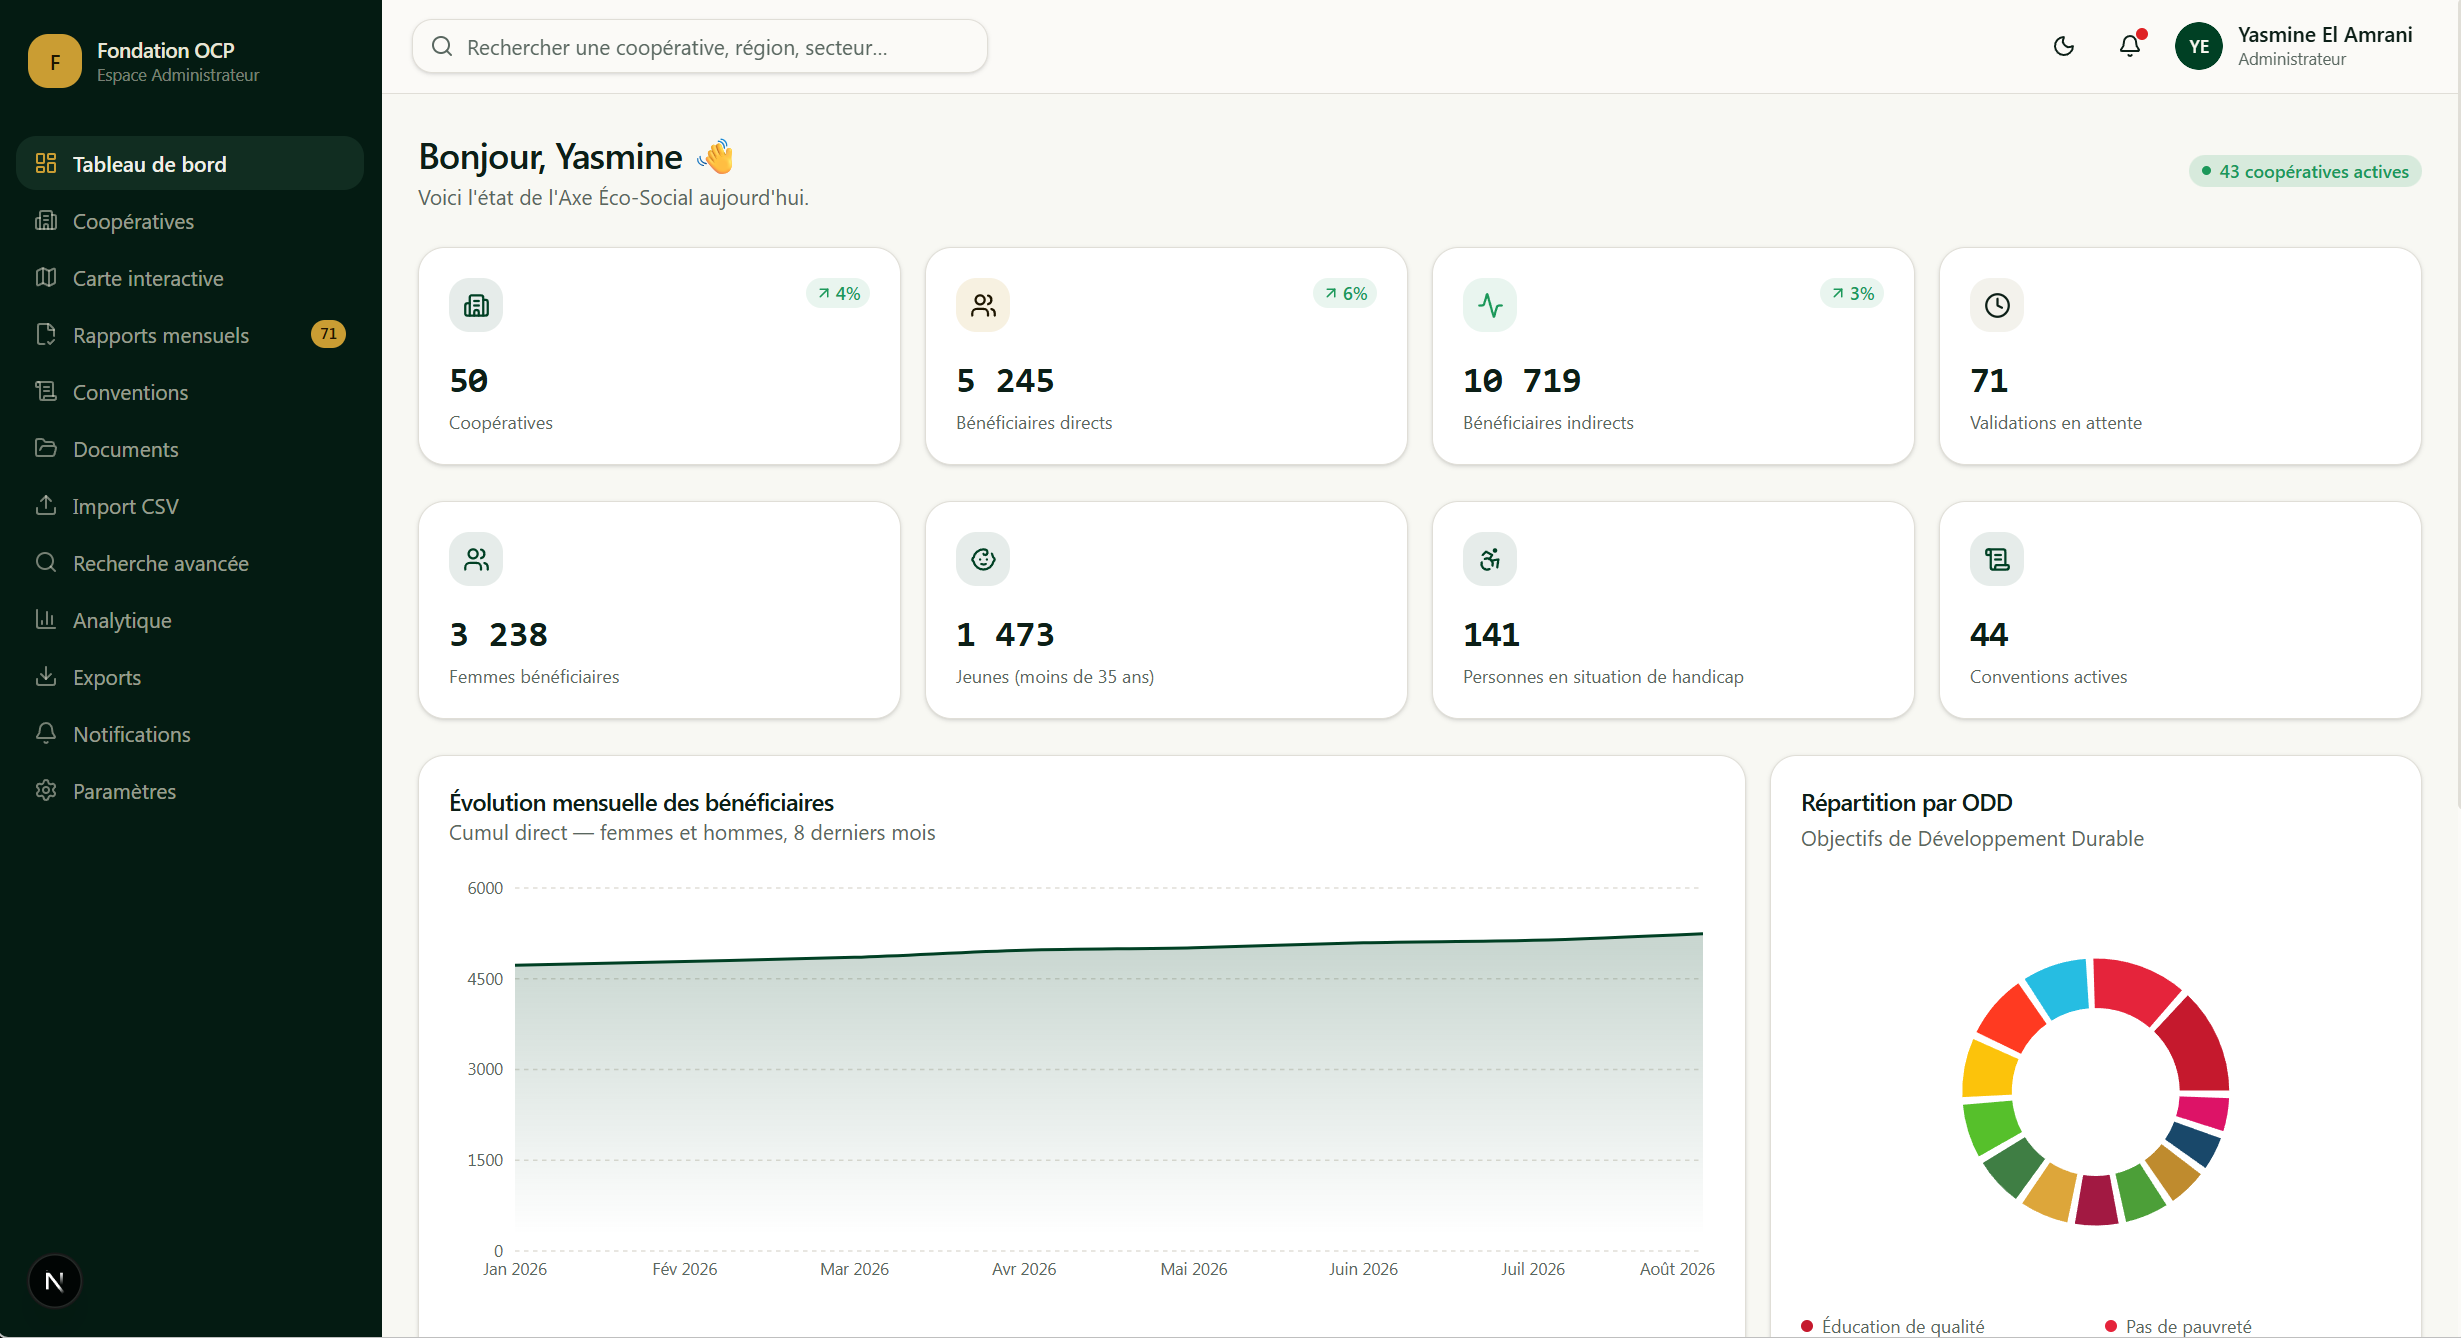
\includegraphics[width=0.90\textwidth]{figures/screenshots/mvp/02_mvp_dashboard.png}
\caption{Tableau de bord général de supervision et indicateurs d'impact}
\label{fig:mvp_02_dash}
\end{figure}

\subsection{Annuaire et gestion des coopératives partenaires}

L'annuaire des coopératives (figure \ref{fig:mvp_03_coop}) permet de gérer l'exhaustivité des 1\,700 coopératives partenaires. L'administrateur peut y filtrer les entités par région, province, secteur d'activité (Artisanat, Agriculture, Argan, Cosmétique, etc.) et statut administratif.

\begin{figure}[H]
\centering
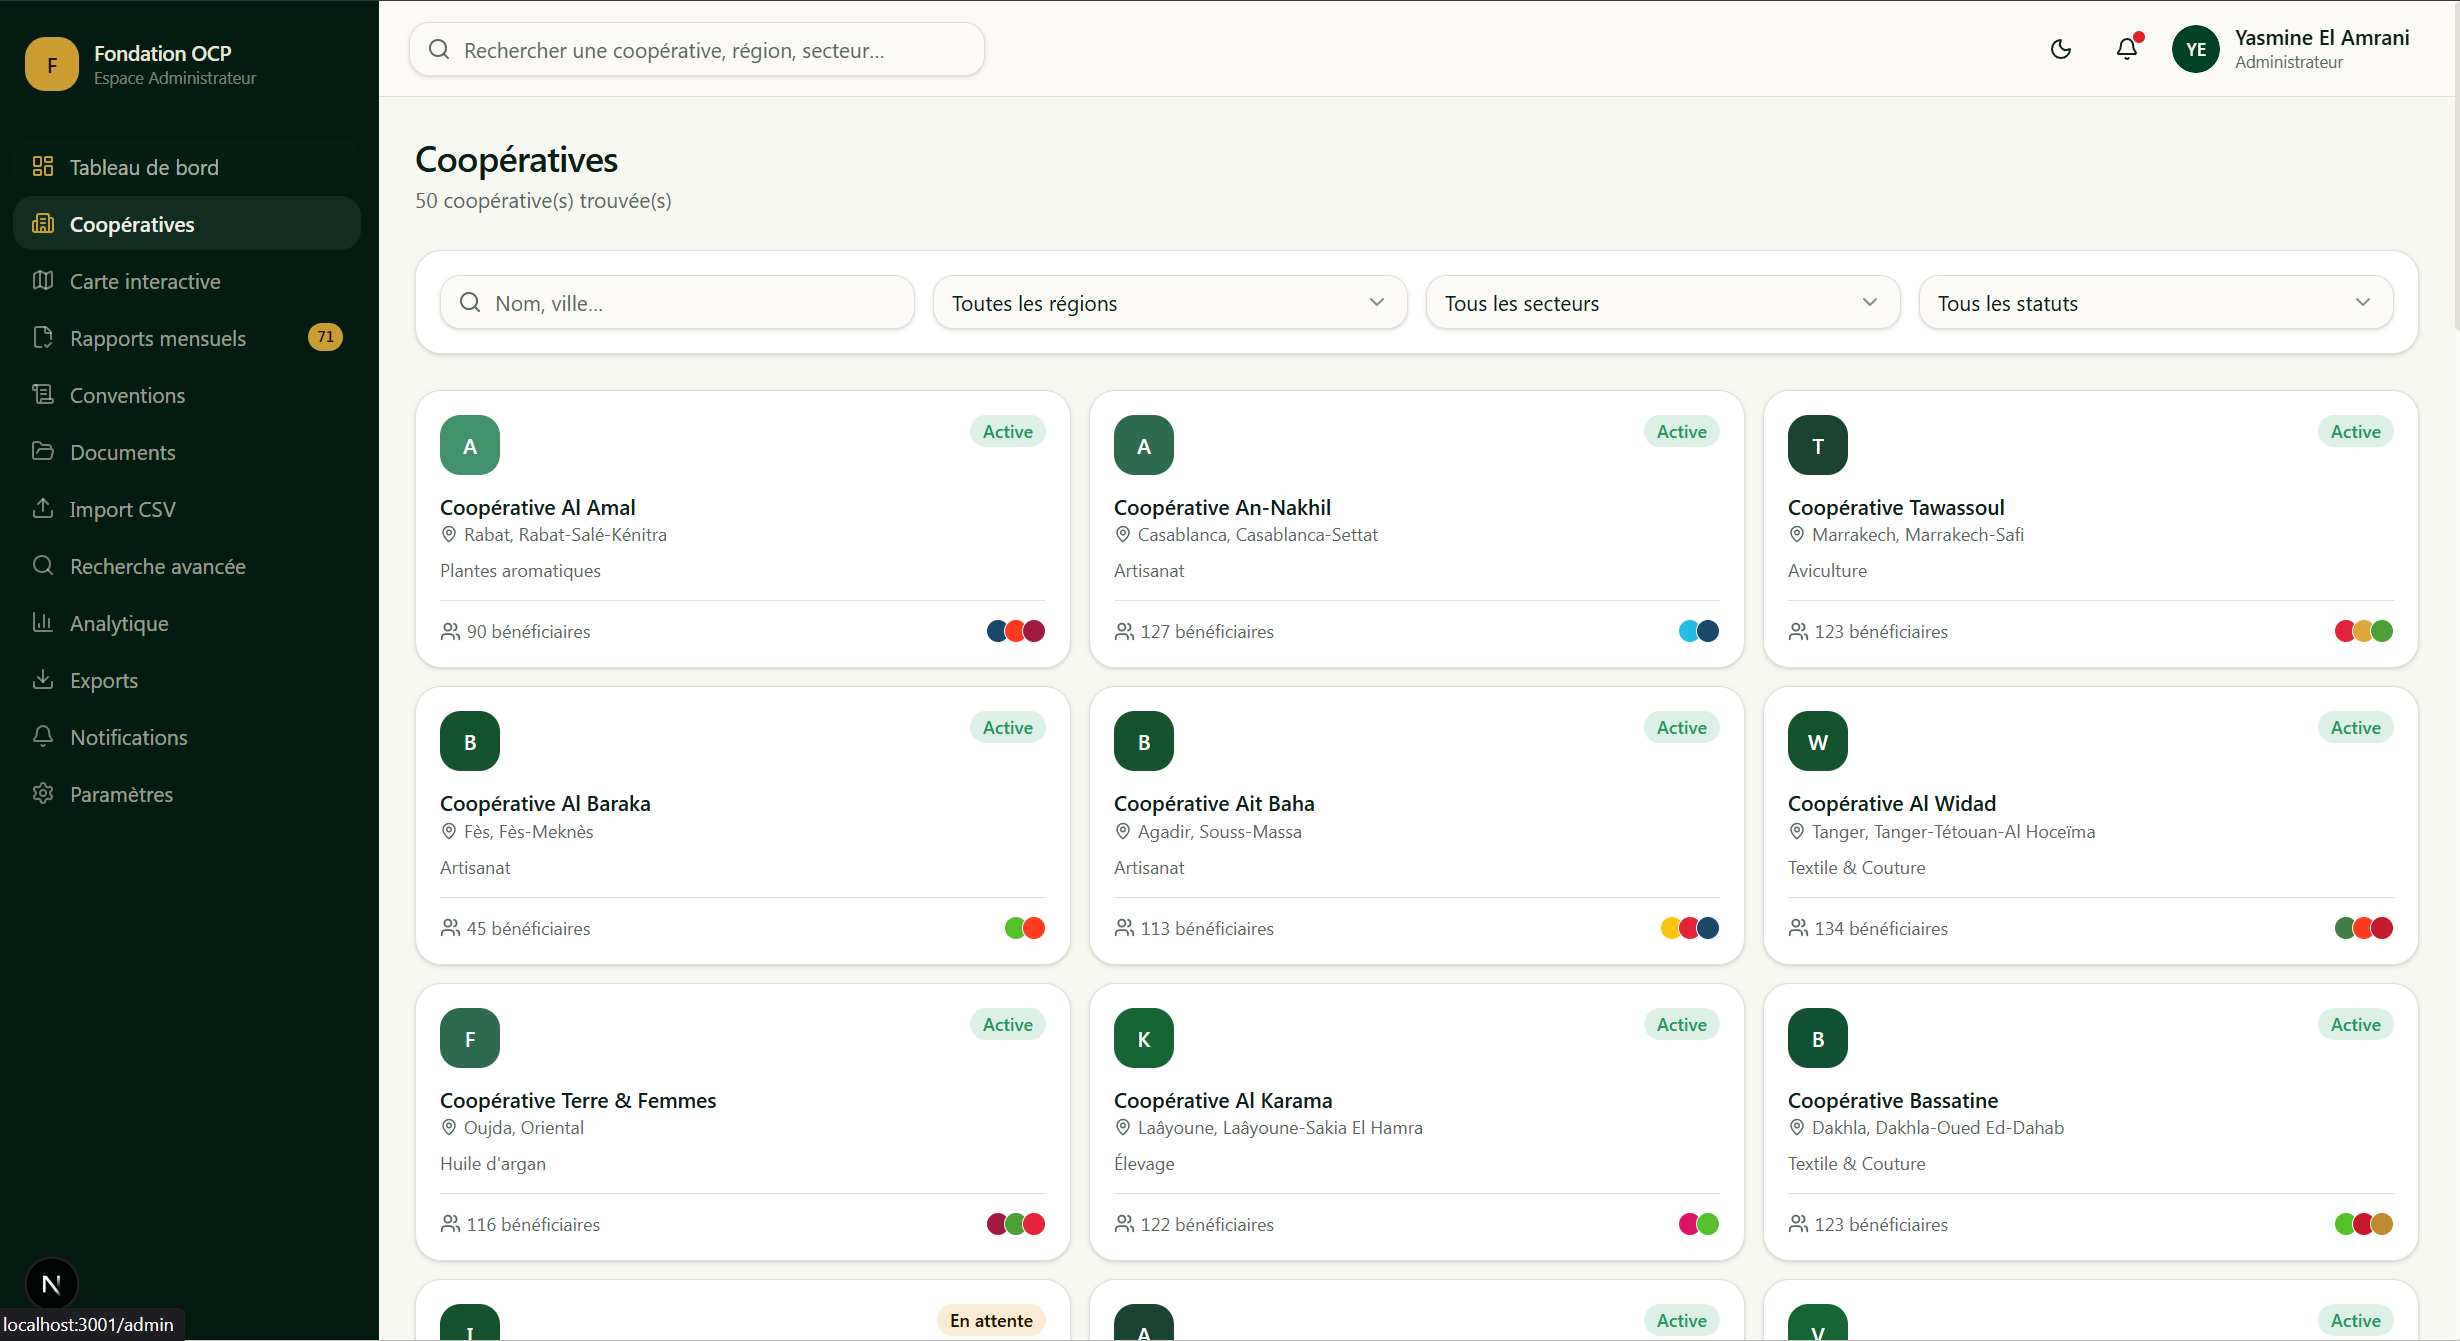
\includegraphics[width=0.90\textwidth]{figures/screenshots/mvp/03_mvp_cooperatives.png}
\caption{Annuaire et gestion détaillée des coopératives partenaires}
\label{fig:mvp_03_coop}
\end{figure}

Chaque ligne permet d'accéder à la fiche individuelle de la coopérative, regroupant ses coordonnées, ses représentants légaux, ses conventions et son historique de déclarations.

\subsection{Cartographie interactive nationale des coopératives}

Le module cartographique (figure \ref{fig:mvp_04_map}) s'appuie sur une carte interactive du Maroc permettant la géolocalisation précise des coopératives et l'analyse territoriale des retombées des programmes de la Fondation OCP.

\begin{figure}[H]
\centering
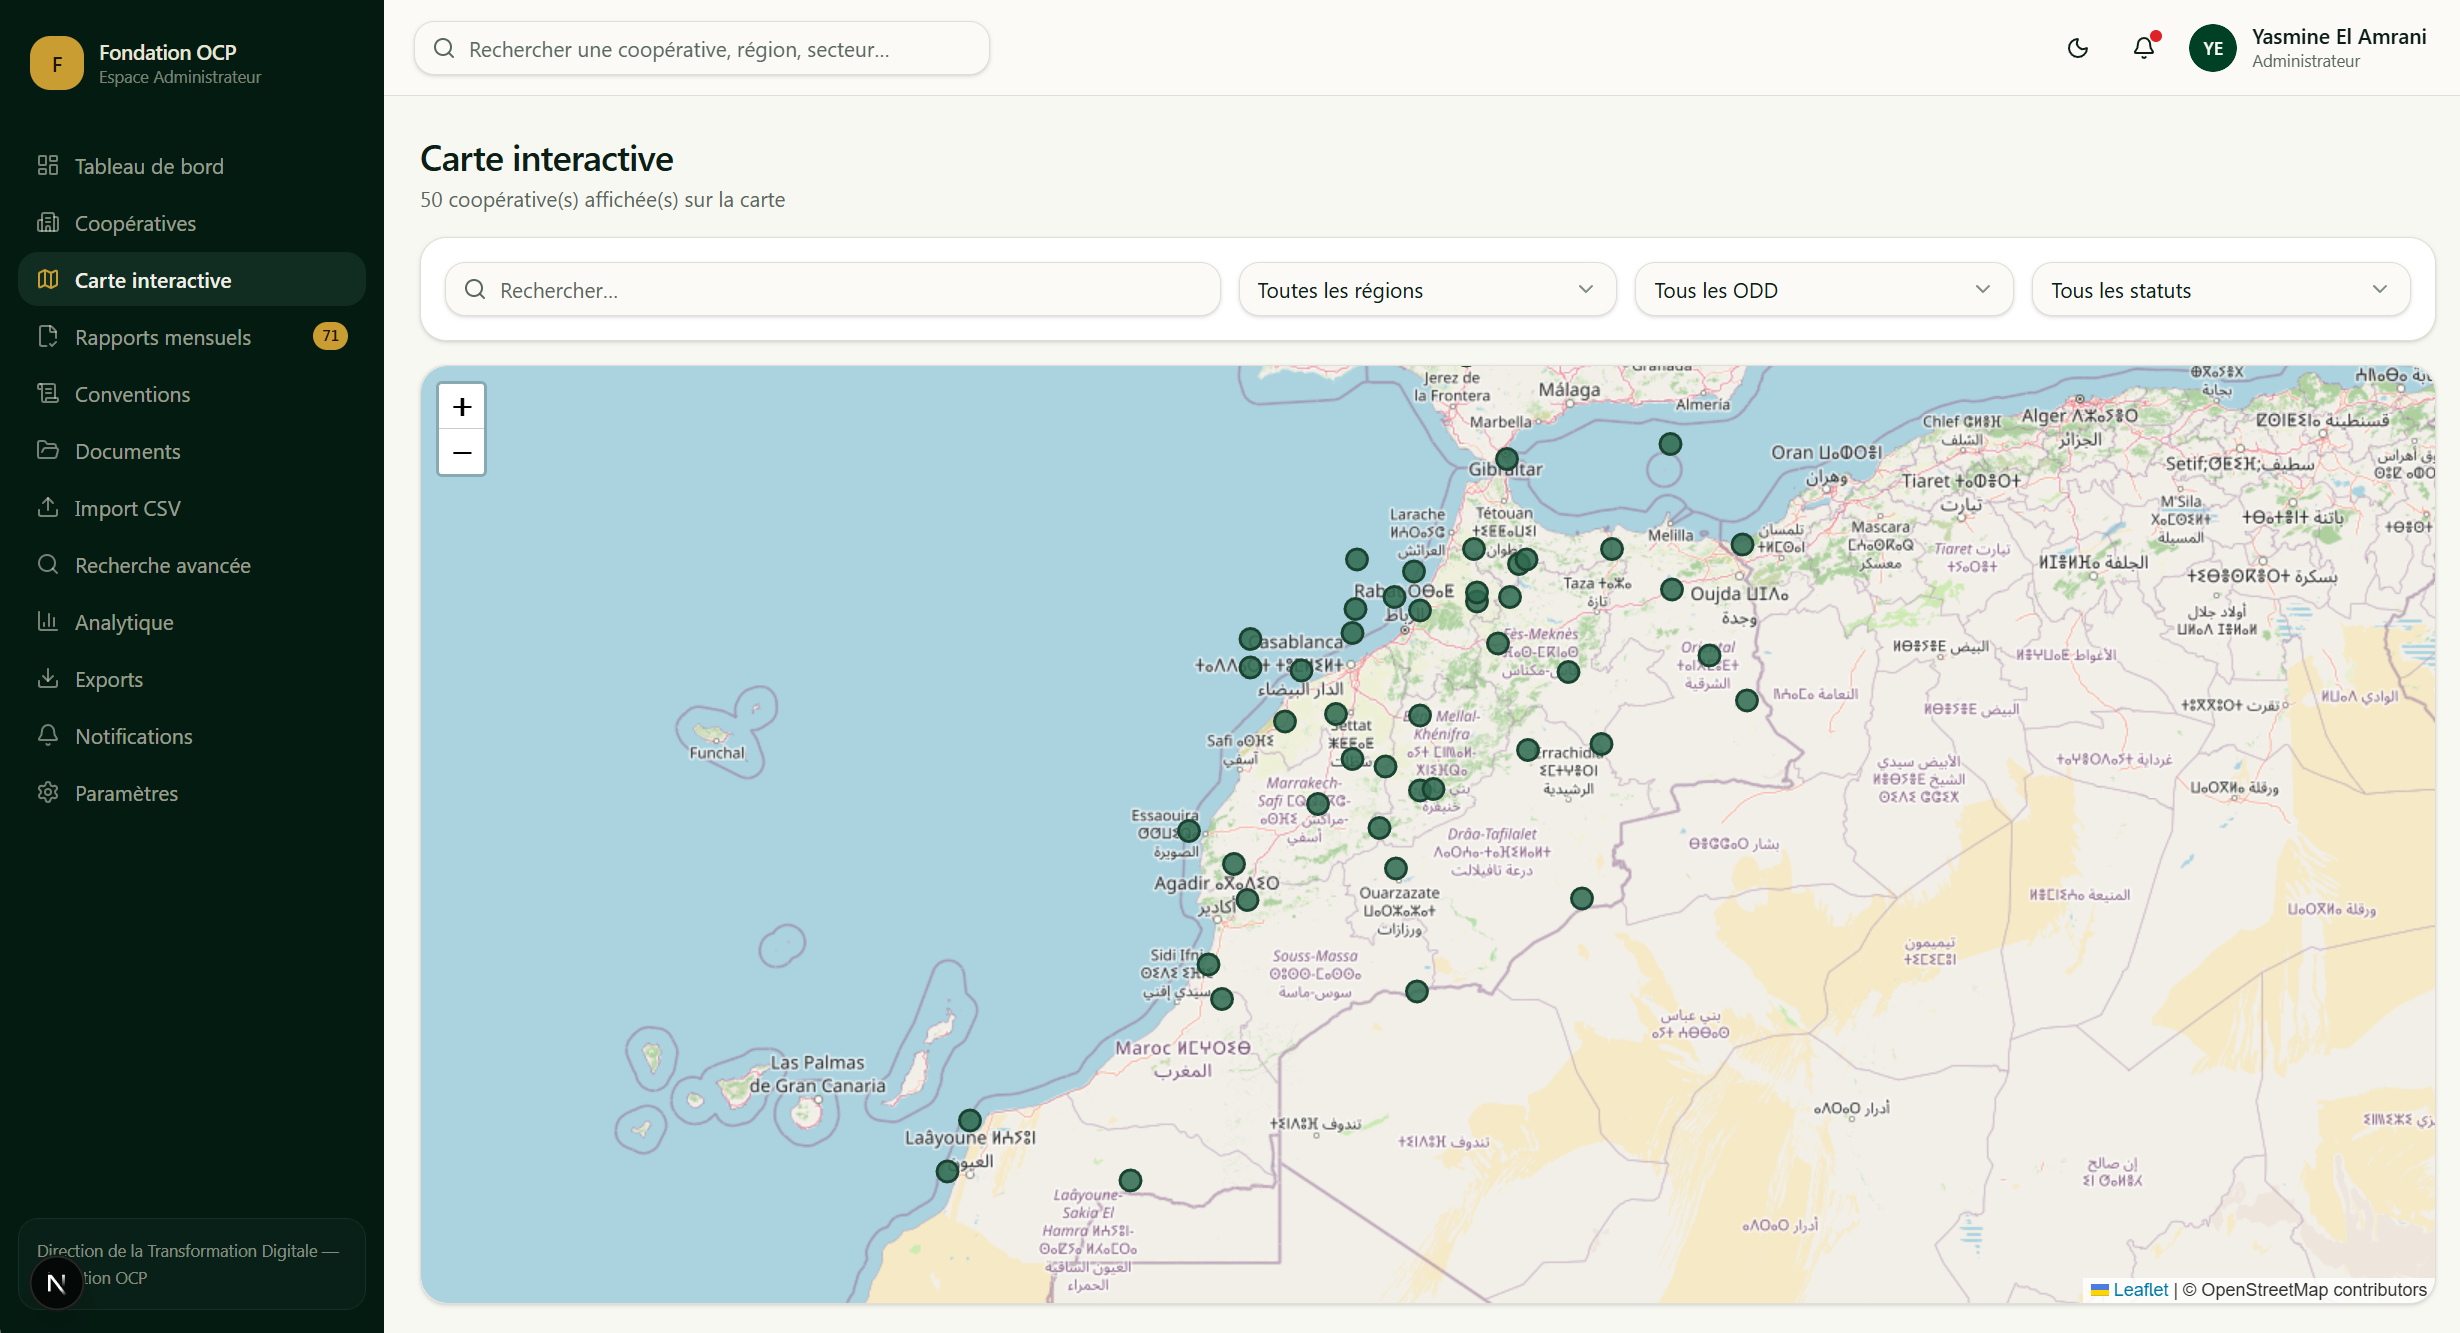
\includegraphics[width=0.90\textwidth]{figures/screenshots/mvp/04_mvp_carte_interactive.png}
\caption{Cartographie interactive nationale des coopératives et bénéficiaires}
\label{fig:mvp_04_map}
\end{figure}

L'interface propose des filtres dynamiques par région et secteur d'activité, affichant des infobulles détaillées lors du survol ou du clic sur chaque point géographique.

\subsection{Suivi et circuit de validation des rapports d'activité mensuels}

Le module de gestion des rapports mensuels (figure \ref{fig:mvp_05_reports}) dématérialise le workflow complet de reporting. Les coopératives y déclarent leurs activités et indicateurs mensuels, tandis que les équipes de la Fondation examinent les soumissions.

\begin{figure}[H]
\centering
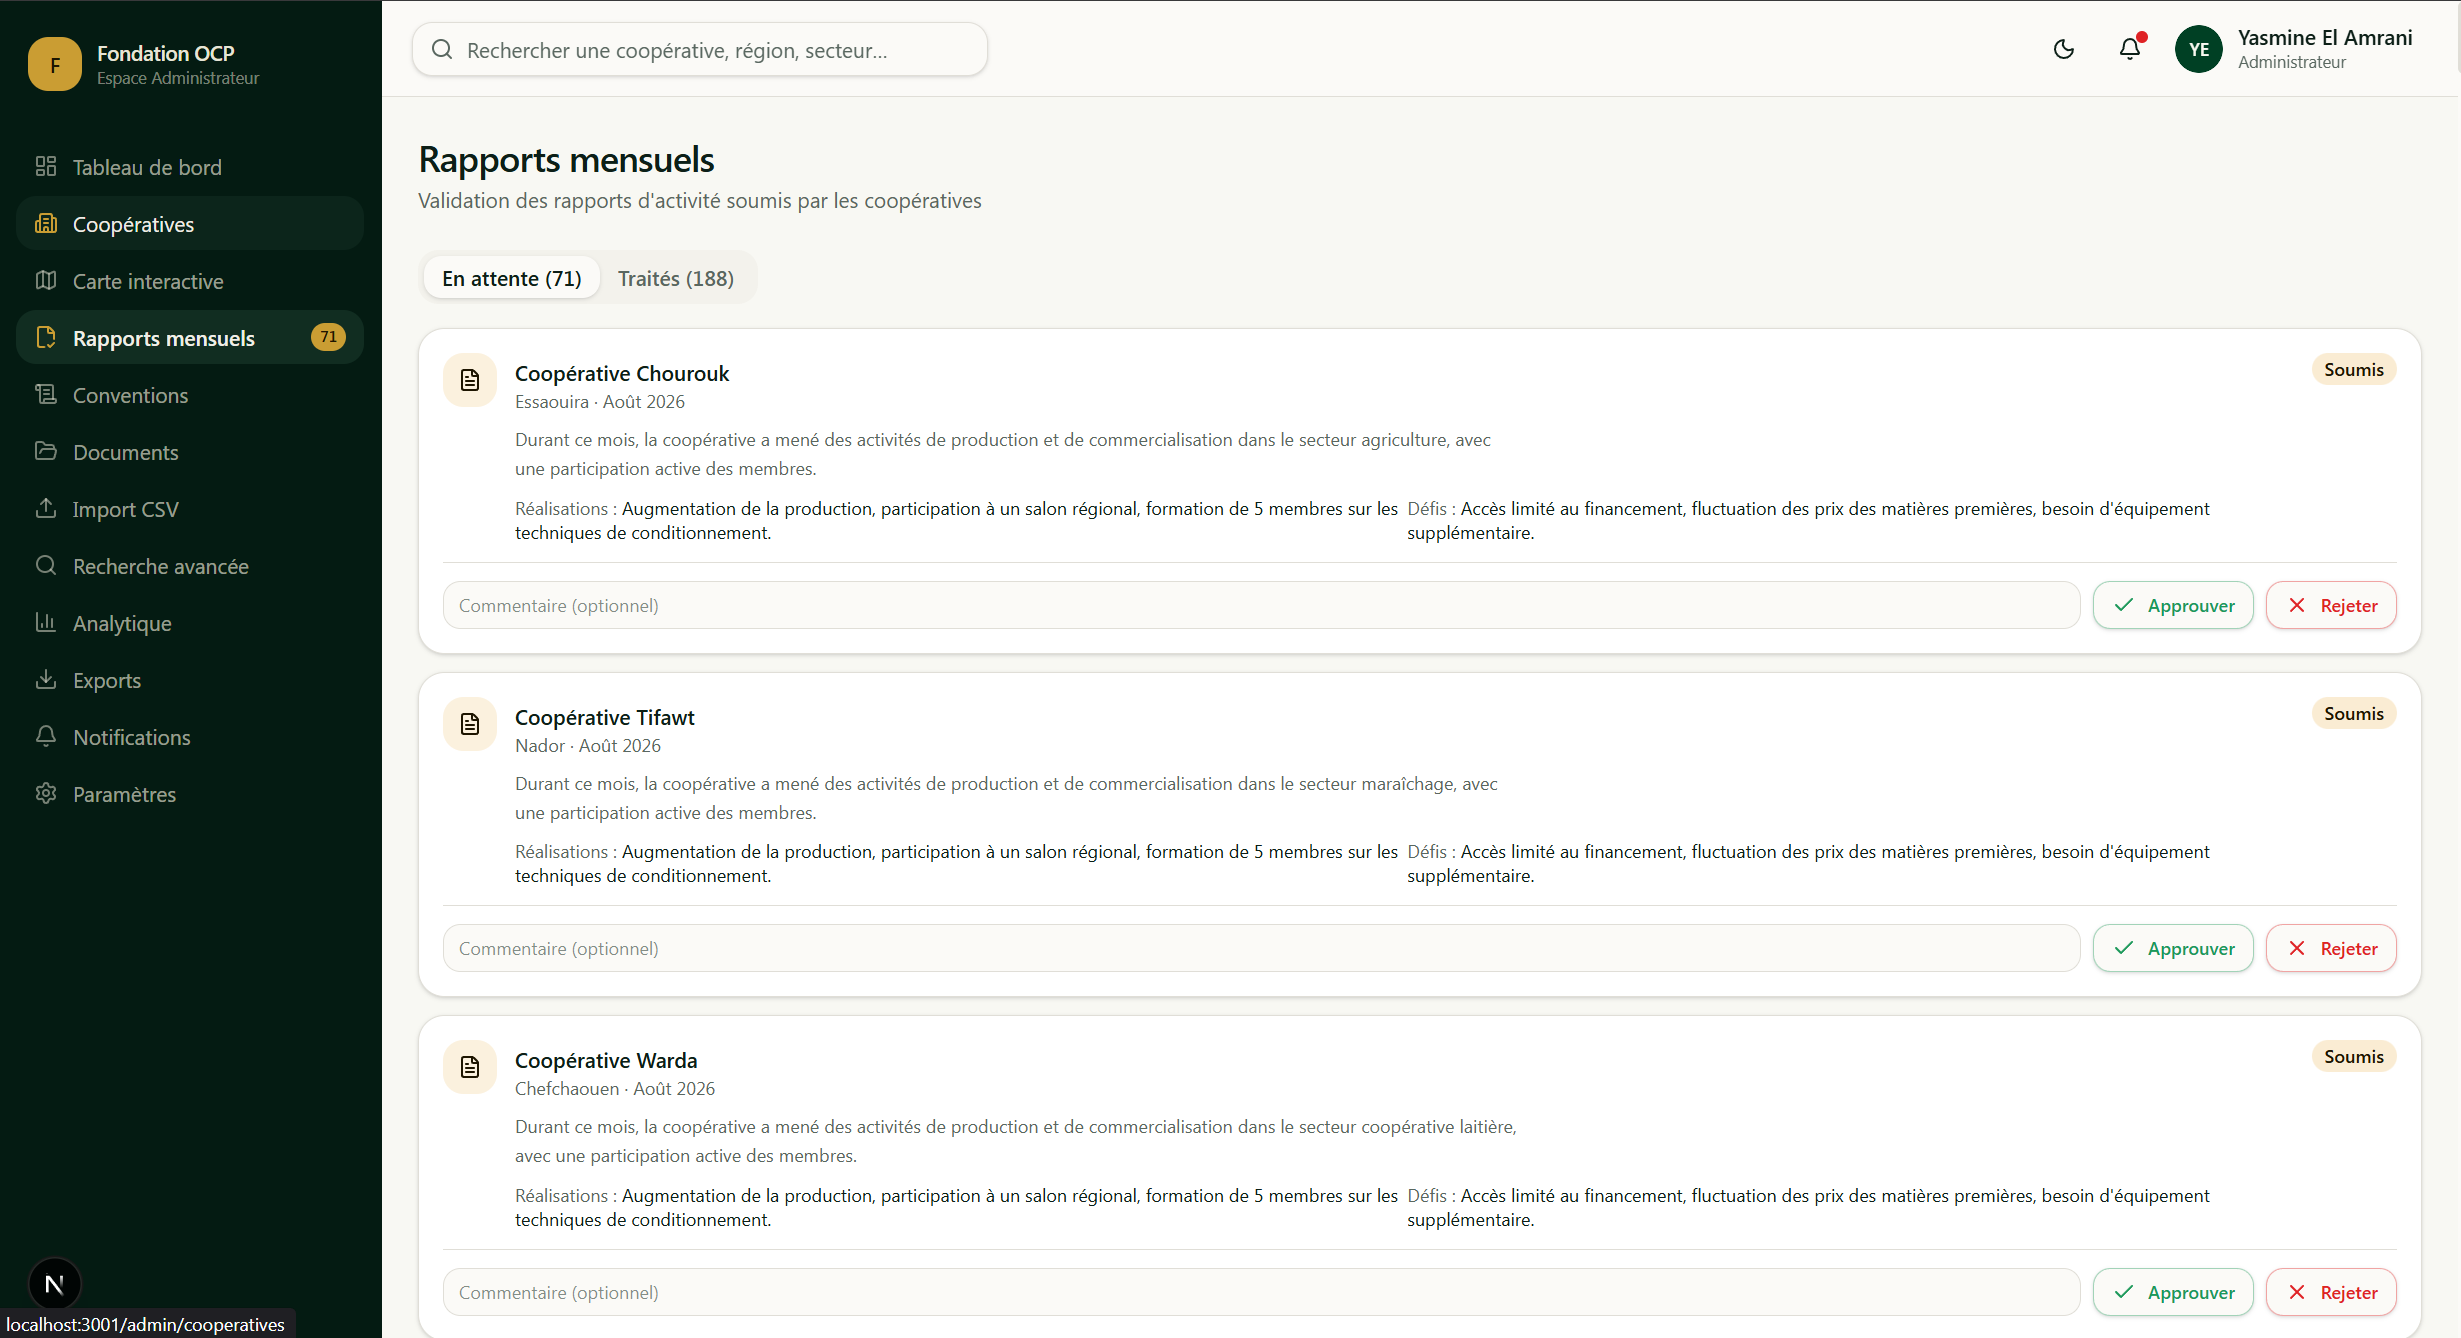
\includegraphics[width=0.90\textwidth]{figures/screenshots/mvp/05_mvp_rapports_mensuels.png}
\caption{Circuit de suivi, validation et rejet motivé des rapports mensuels}
\label{fig:mvp_05_reports}
\end{figure}

L'administrateur dispose des options de validation formelle ou de rejet avec obligation de renseigner un motif explicite, consigné dans le journal d'audit.

\subsection{Suivi des conventions de partenariat et gestion budgétaire}

L'interface de gestion des conventions (figure \ref{fig:mvp_06_conv}) assure le suivi administratif et financier des partenariats conclus entre la Fondation OCP et les coopératives.

\begin{figure}[H]
\centering
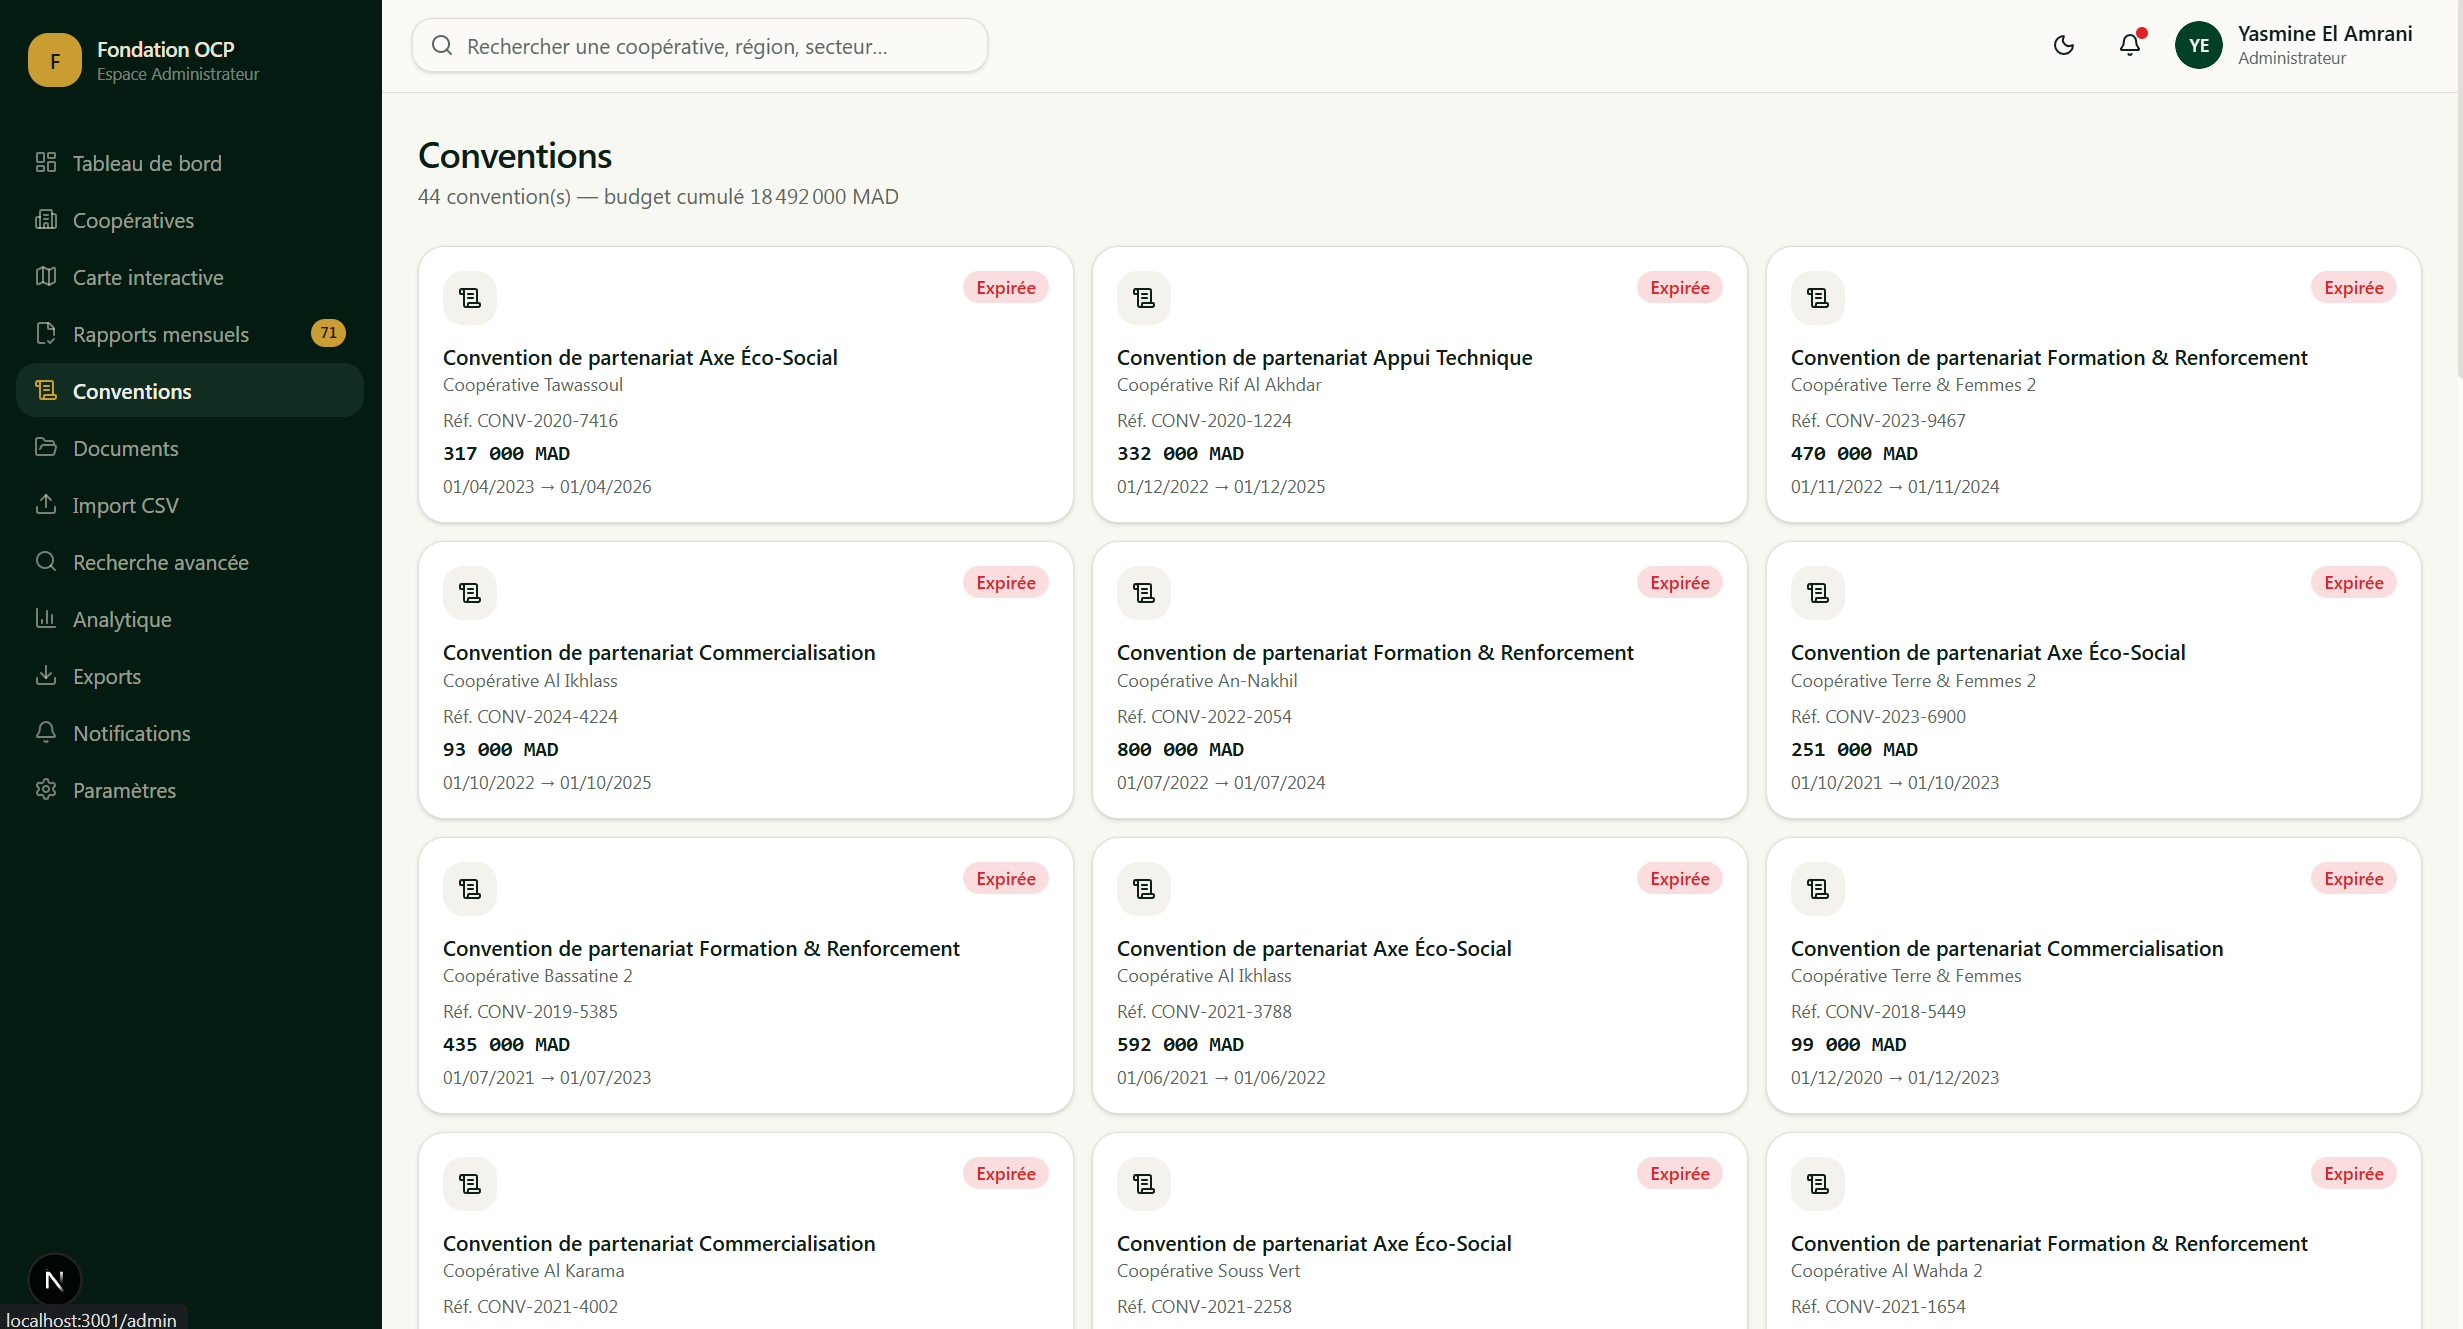
\includegraphics[width=0.90\textwidth]{figures/screenshots/mvp/06_mvp_conventions.png}
\caption{Gestion des conventions de partenariat et suivi des engagements budgétaires}
\label{fig:mvp_06_conv}
\end{figure}

Elle permet de suivre les dates d'effet, les échéances, les montants engagés, les budgets décaissés et les pièces contractuelles associées.

\subsection{Gestion électronique de documents (GED) et pièces justificatives}

Le module documentaire GED (figure \ref{fig:mvp_07_ged}) centralise le dépôt, le stockage sécurisé et la validation des pièces justificatives (statuts légaux, PV d'assemblées générales, listes d'émargement, attestations de versement).

\begin{figure}[H]
\centering
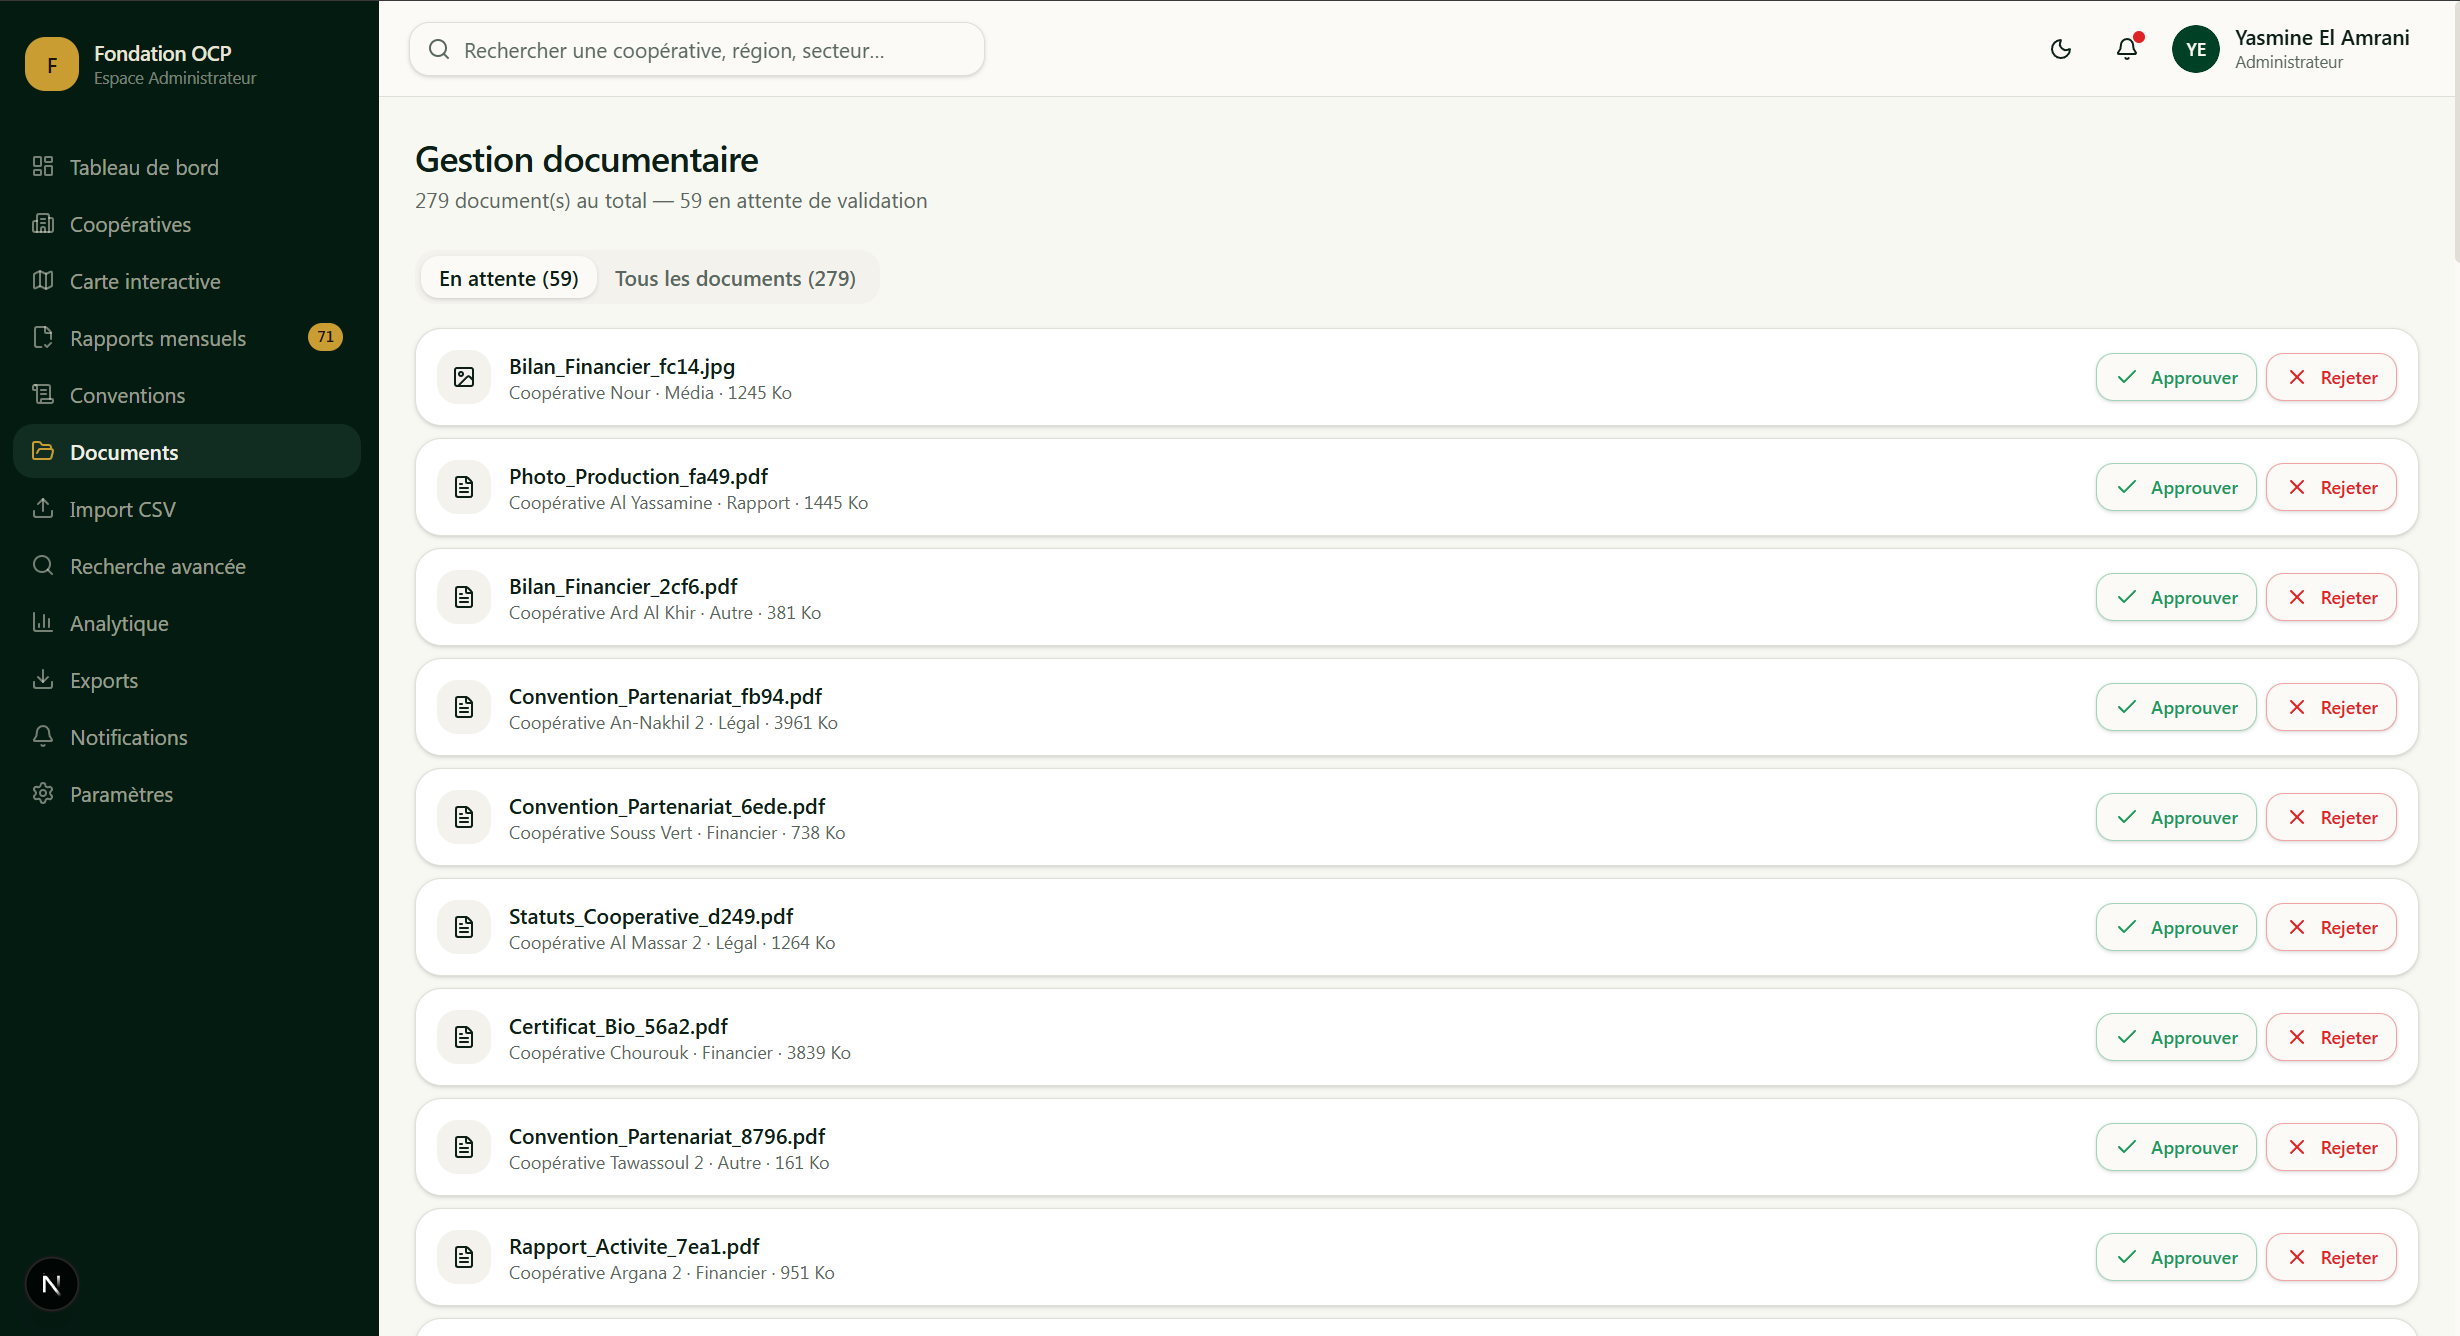
\includegraphics[width=0.90\textwidth]{figures/screenshots/mvp/07_mvp_documents.png}
\caption{Module de Gestion Électronique des Documents (GED) et validation des pièces}
\label{fig:mvp_07_ged}
\end{figure}

Le système applique des contrôles stricts sur les types de fichiers (PDF, images), vérifie l'absence de scripts malveillants et garantit l'intégrité des pièces déposées.

\subsection{Importation massive des données de coopératives par fichier CSV}

Pour faciliter l'initialisation du réseau ou la mise à jour périodique par lots, le MVP intègre un moteur d'importation de fichiers CSV (figure \ref{fig:mvp_08_import}).

\begin{figure}[H]
\centering
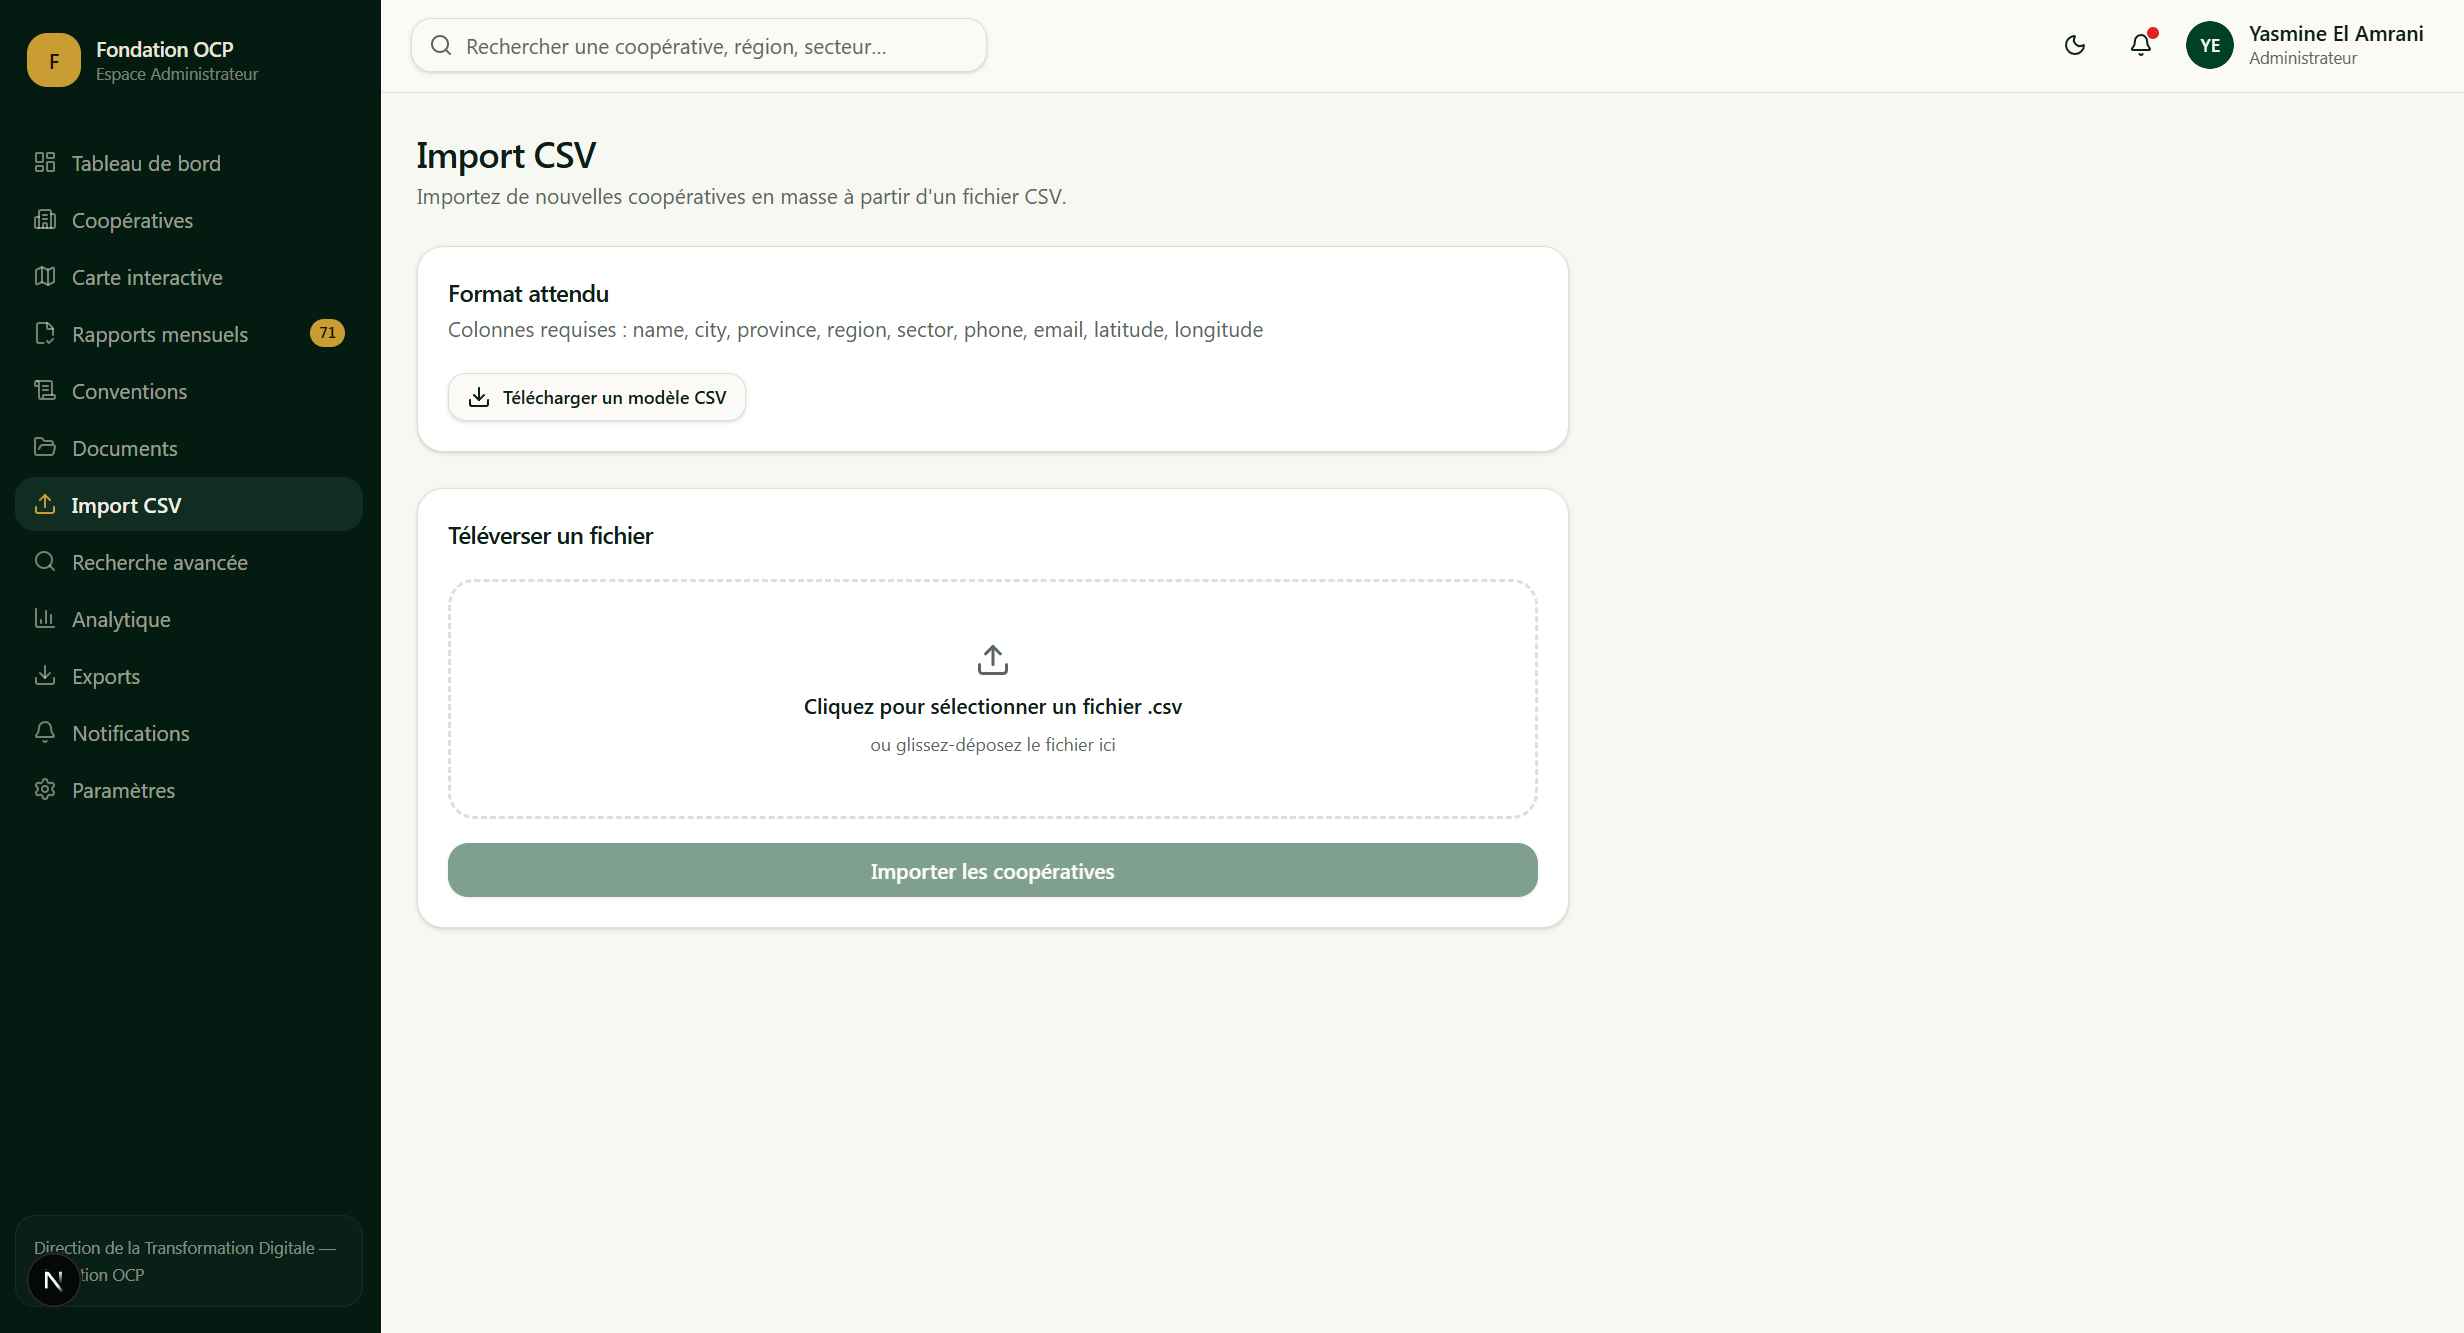
\includegraphics[width=0.90\textwidth]{figures/screenshots/mvp/08_mvp_import_csv.png}
\caption{Interface d'importation massive des coopératives via fichier CSV}
\label{fig:mvp_08_import}
\end{figure}

Ce module propose un modèle de données type, analyse les lignes importées, détecte les anomalies de format et valide l'intégrité avant insertion en base.

\subsection{Moteur de recherche multicritère avancée et filtrage dynamique}

L'interface de recherche avancée (figure \ref{fig:mvp_09_search}) permet aux administrateurs de croiser de multiples critères de recherche (région, secteur, plage de bénéficiaires, conformité des déclarations, statut de convention).

\begin{figure}[H]
\centering
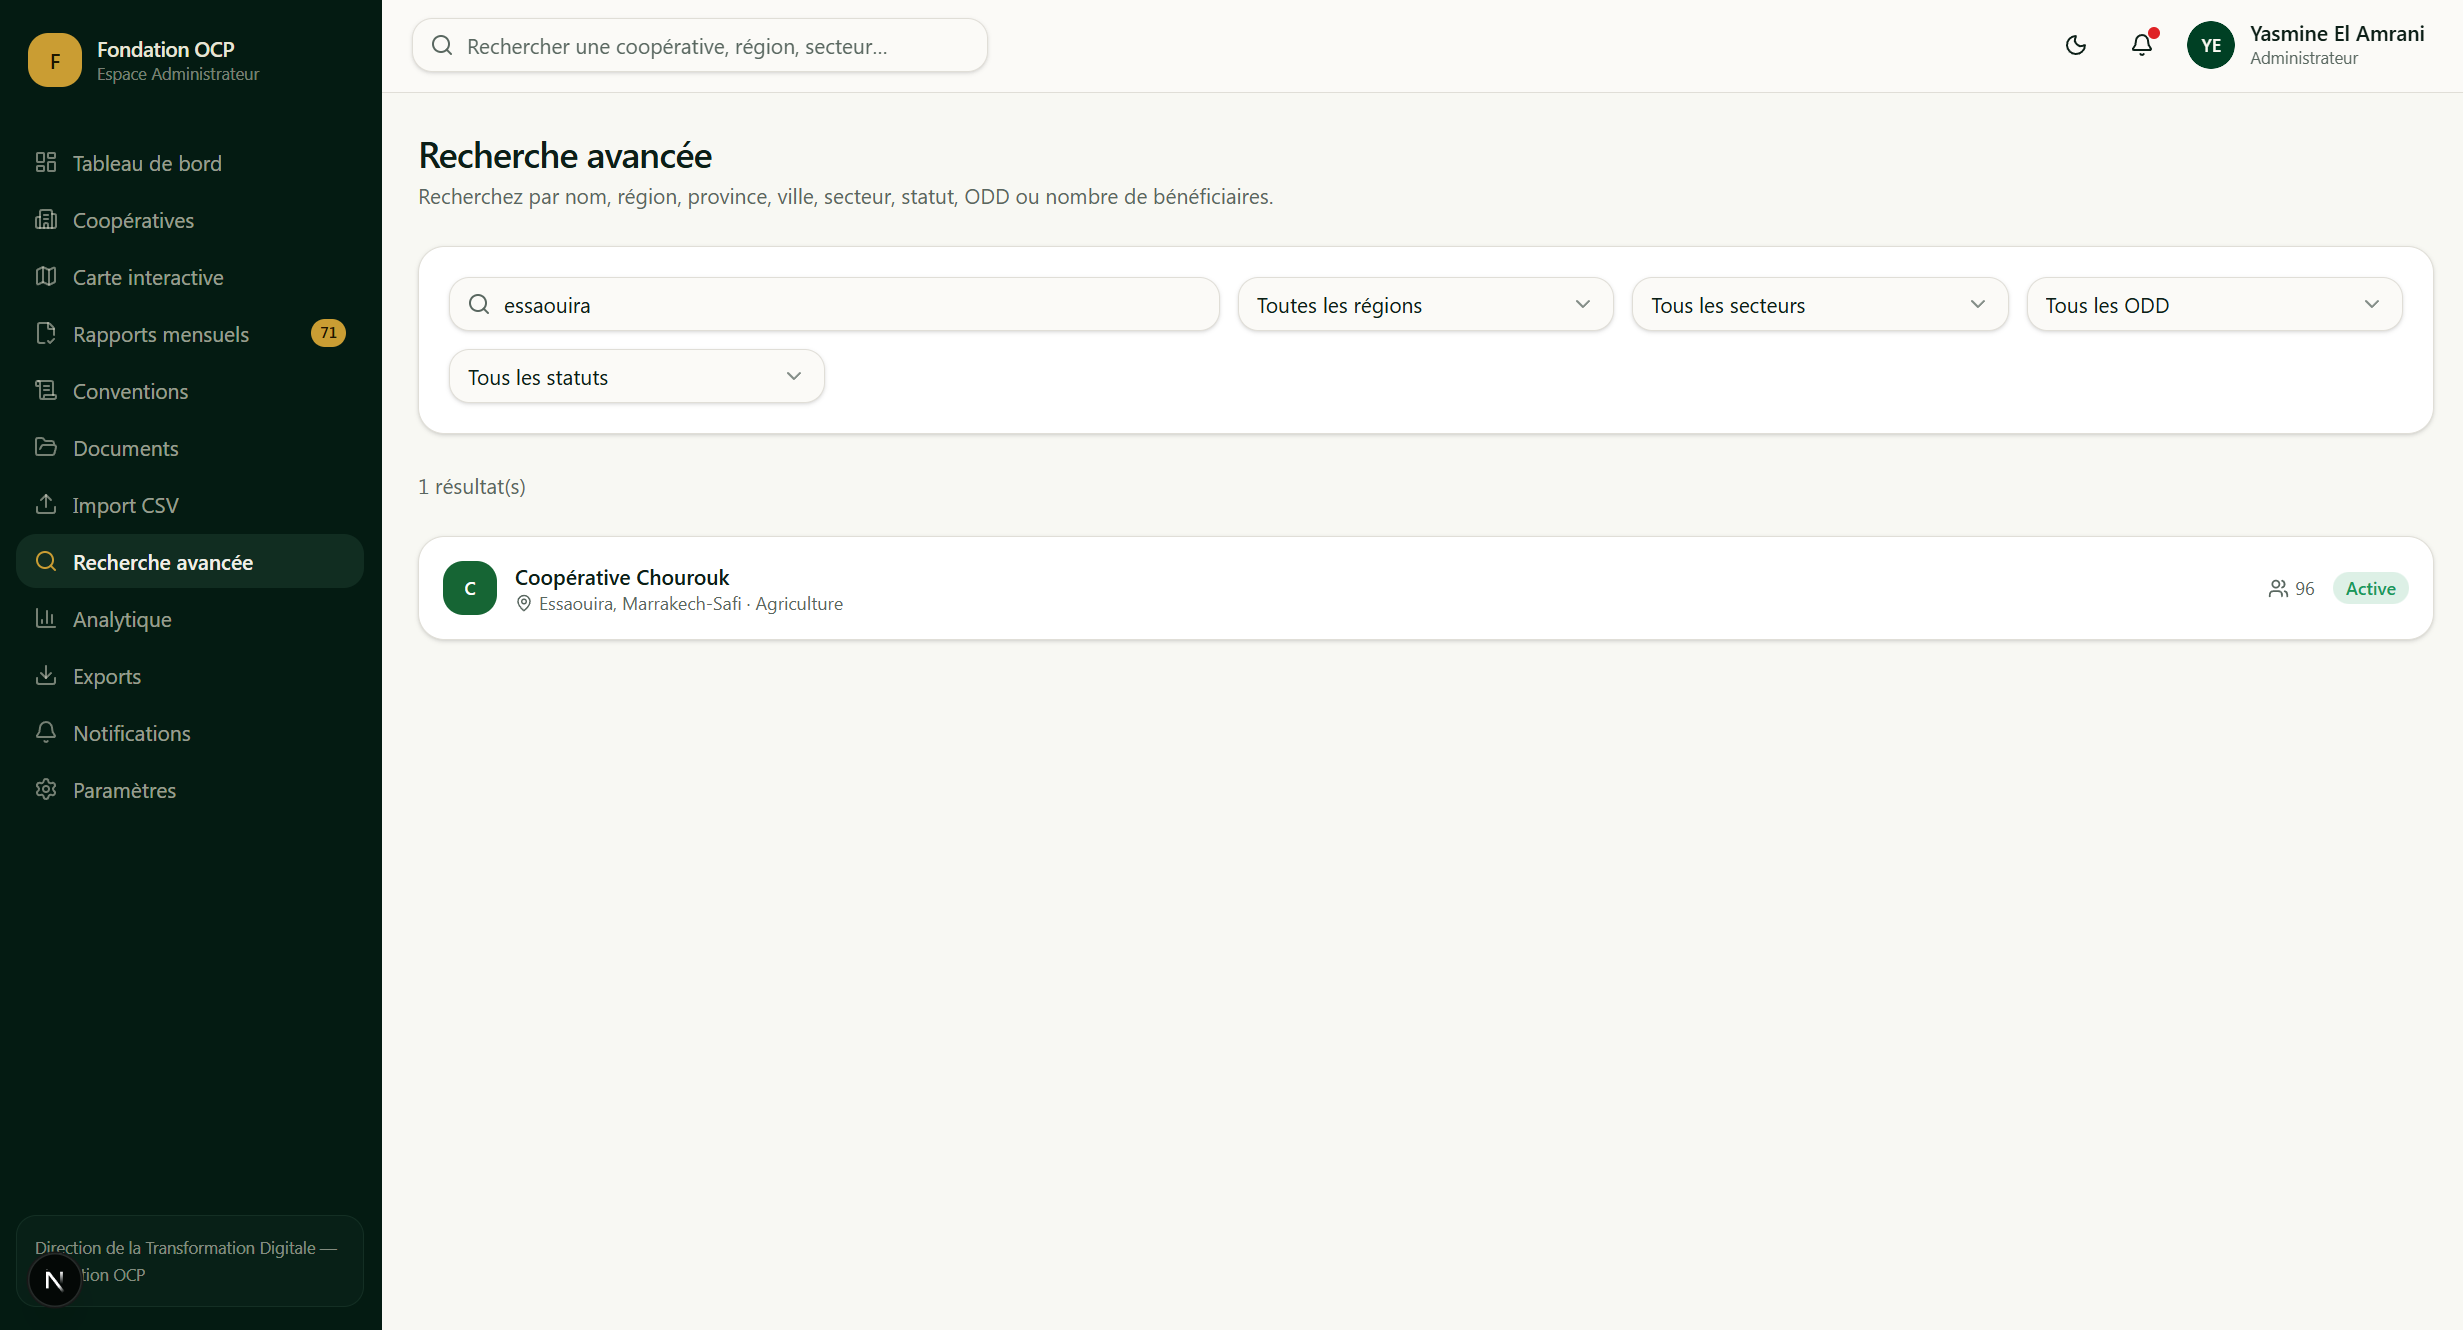
\includegraphics[width=0.90\textwidth]{figures/screenshots/mvp/09_mvp_recherche_avancee.png}
\caption{Moteur de recherche multicritère avancée et filtrage combiné}
\label{fig:mvp_09_search}
\end{figure}

Cette fonctionnalité répond au besoin d'audit et d'extraction ciblée exprimé par les directions métiers de la Fondation.

\subsection{Tableau de bord analytique avancé (Parité, ESG et ODD)}

L'espace analytique approfondi (figure \ref{fig:mvp_10_analytics}) fournit des visualisations détaillées dédiées aux indicateurs d'impact durable : ratio de parité femmes/hommes, inclusion des jeunes ruraux, personnes en situation de handicap et alignement avec les objectifs ESG.

\begin{figure}[H]
\centering
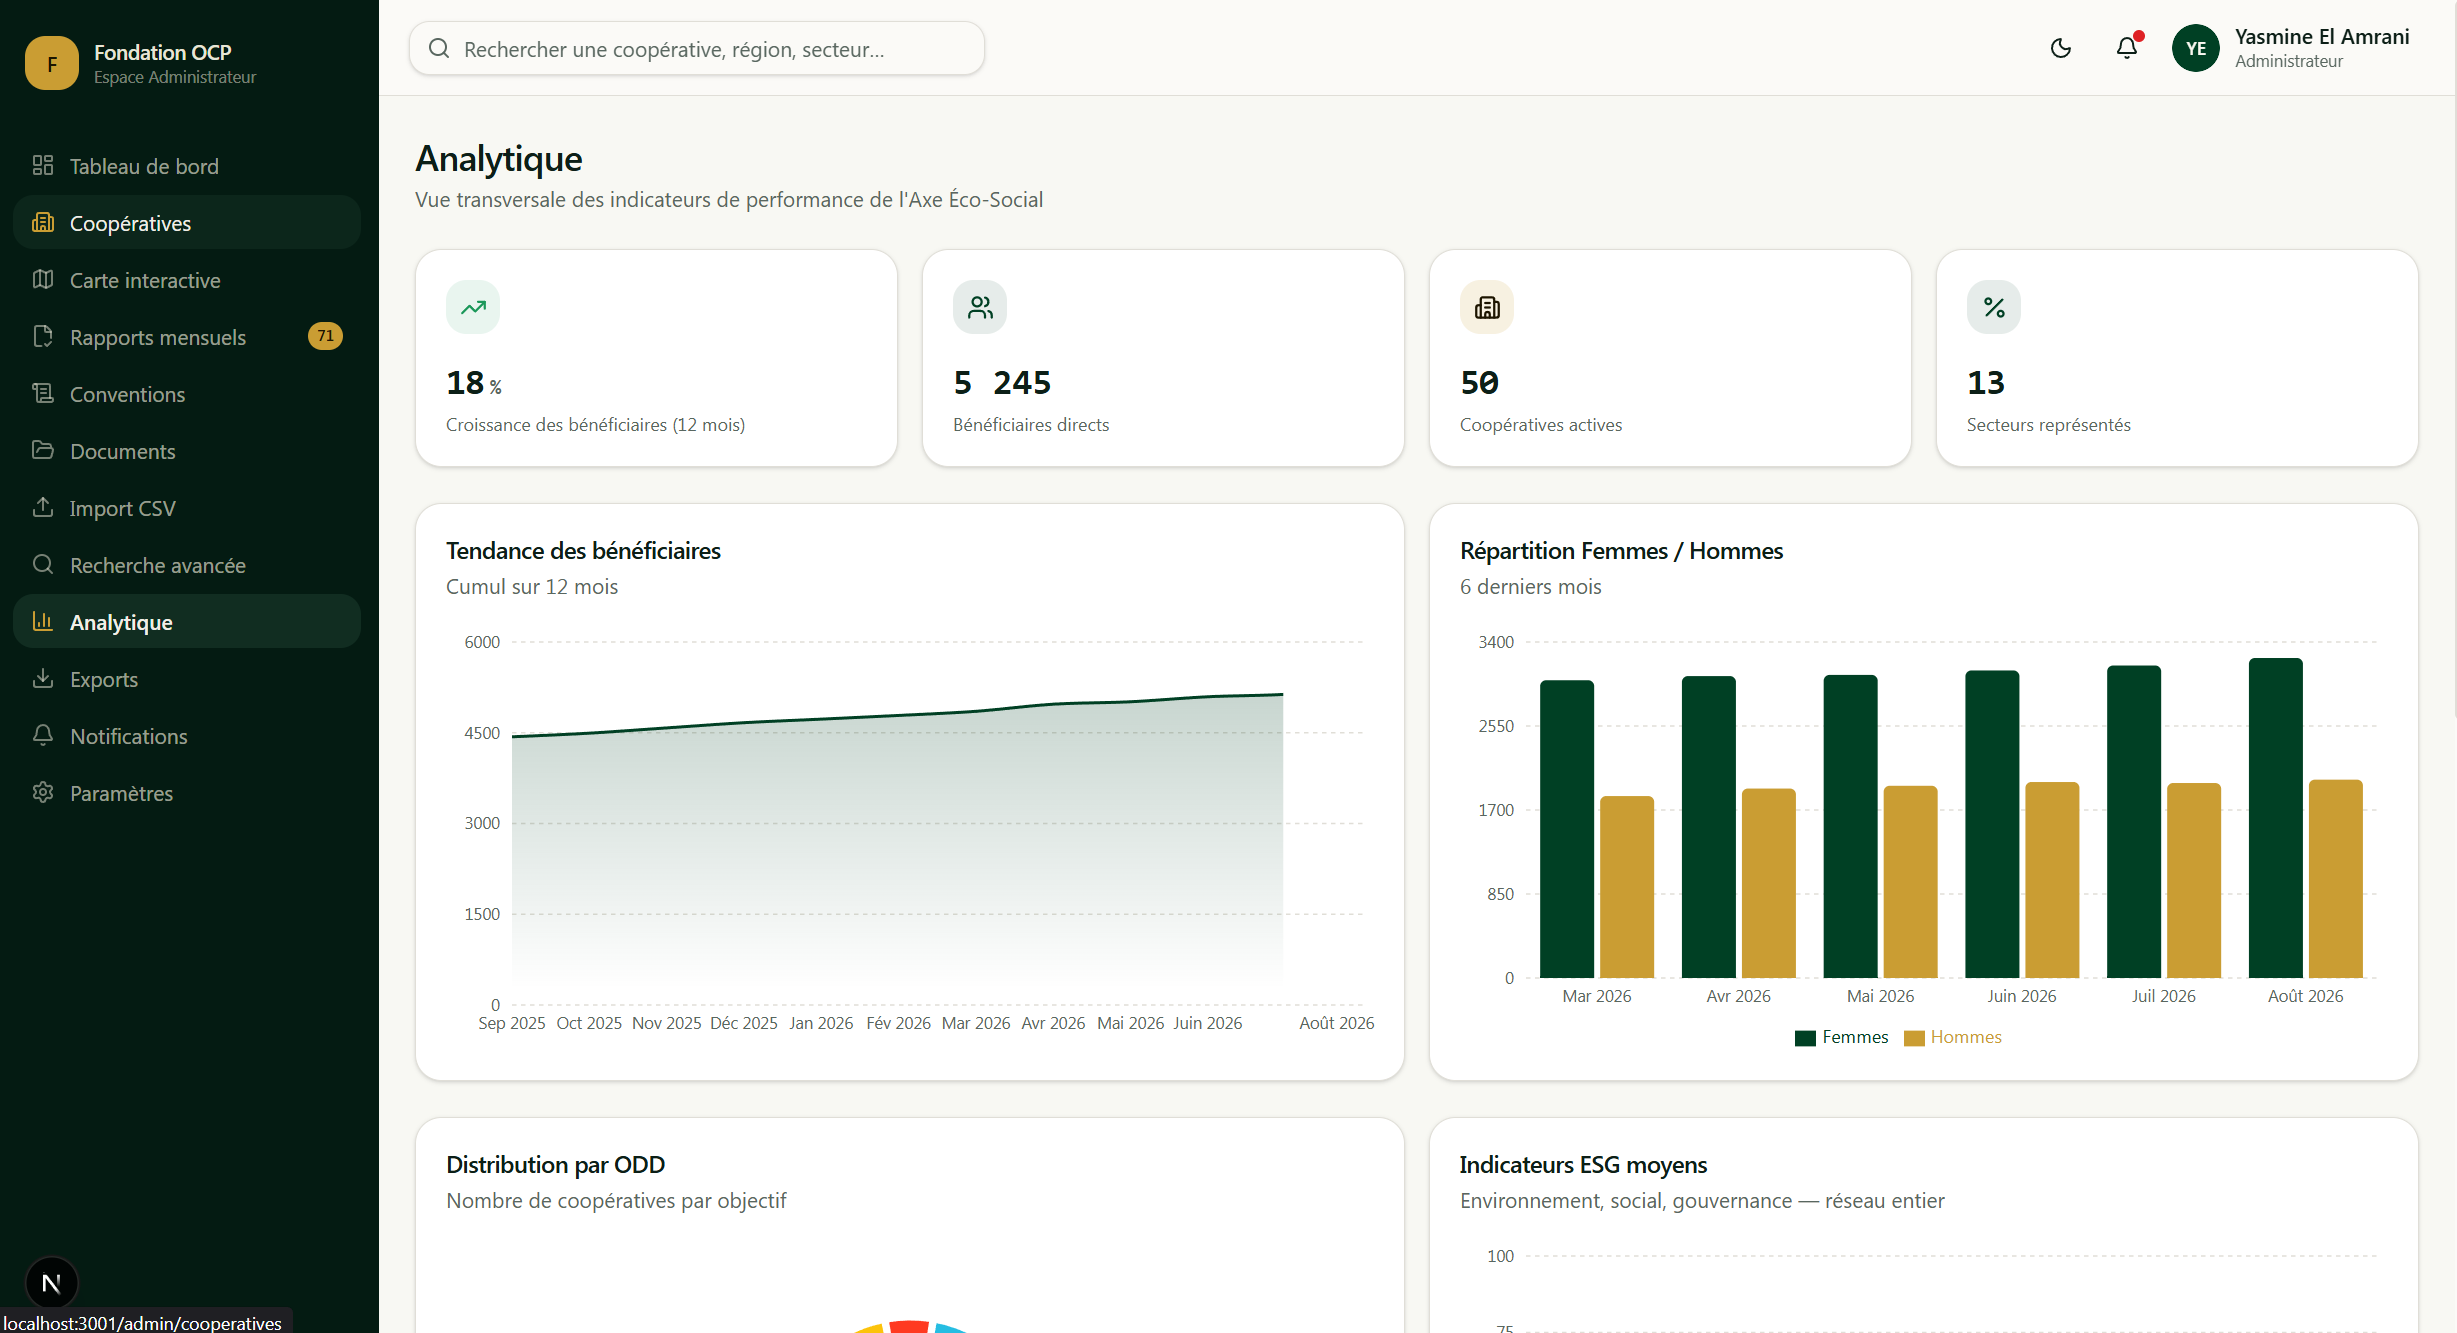
\includegraphics[width=0.90\textwidth]{figures/screenshots/mvp/10_mvp_analytique.png}
\caption{Tableau de bord analytique avancé : parité de genre, impact ESG et ODD}
\label{fig:mvp_10_analytics}
\end{figure}

\subsection{Module d'exportation multi-format des données consolidées}

Le module d'exportation (figure \ref{fig:mvp_11_export}) permet de générer des extractions des données globales ou filtrées sous différents formats normalisés : CSV, tableur Excel (.xlsx) et rapport de synthèse au format PDF.

\begin{figure}[H]
\centering
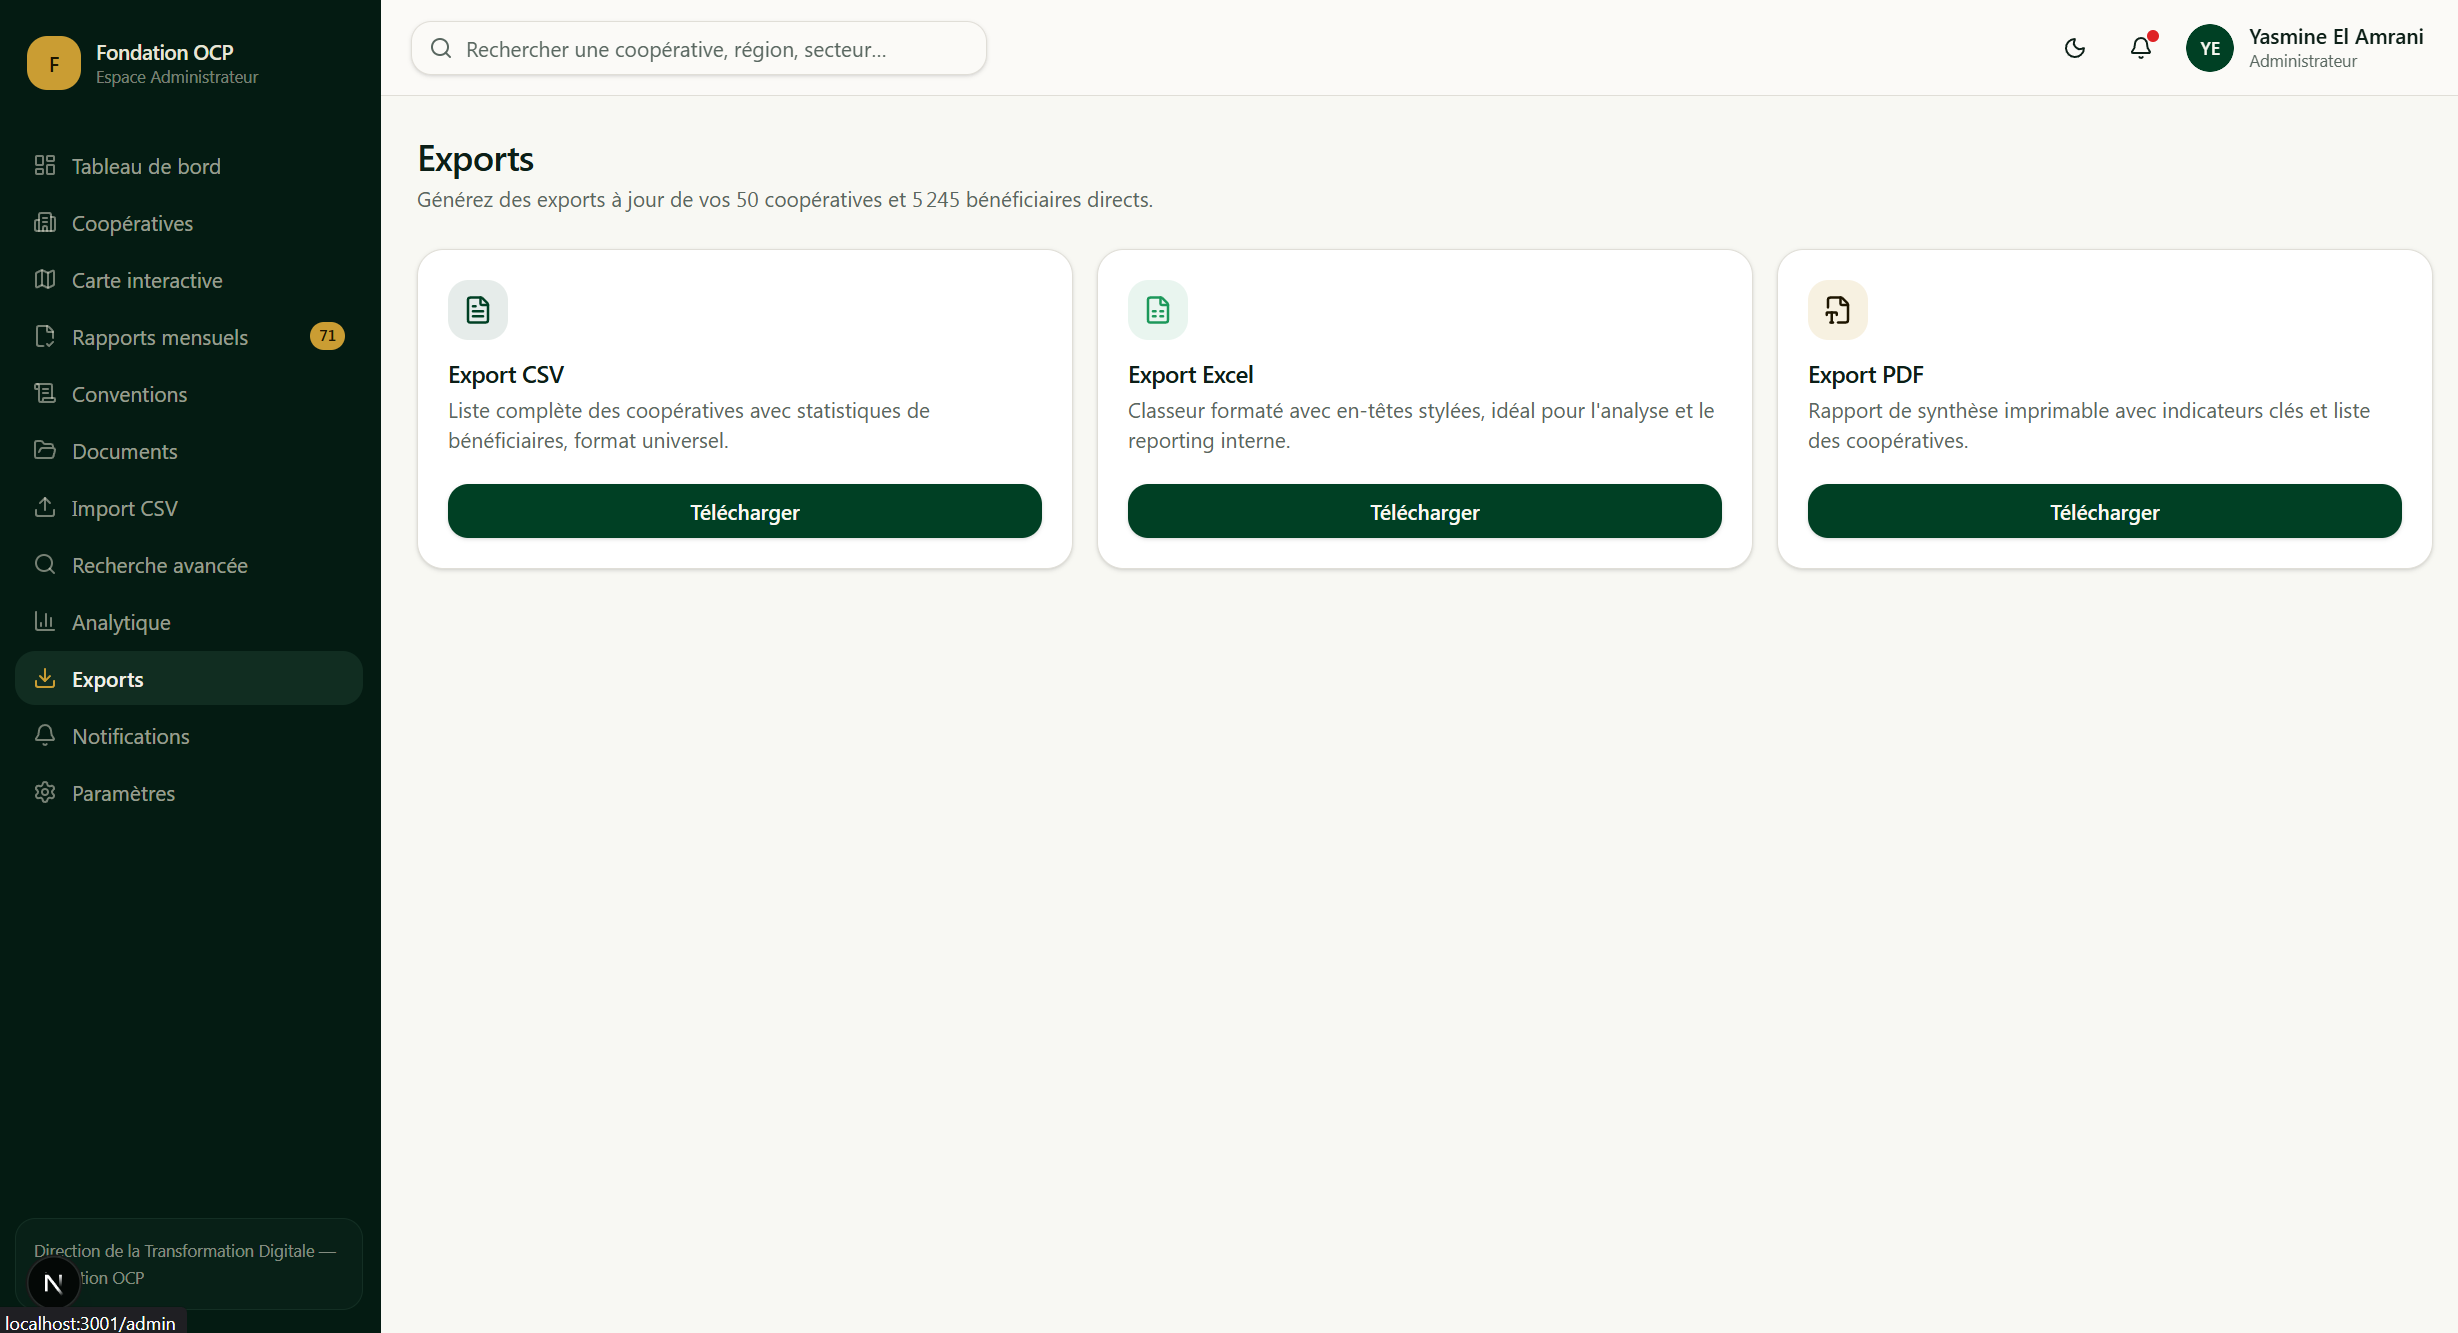
\includegraphics[width=0.90\textwidth]{figures/screenshots/mvp/11_mvp_exports.png}
\caption{Interface d'exportation multi-format des données et synthèses d'impact}
\label{fig:mvp_11_export}
\end{figure}

\subsection{Centre de notifications et alertes de soumission}

Le centre de notifications (figure \ref{fig:mvp_12_notif}) assure le suivi événementiel des processus opérationnels en notifiant les administrateurs des nouveaux rapports déposés et en alertant les coopératives en cas de rejet motivé ou d'échéance imminente.

\begin{figure}[H]
\centering
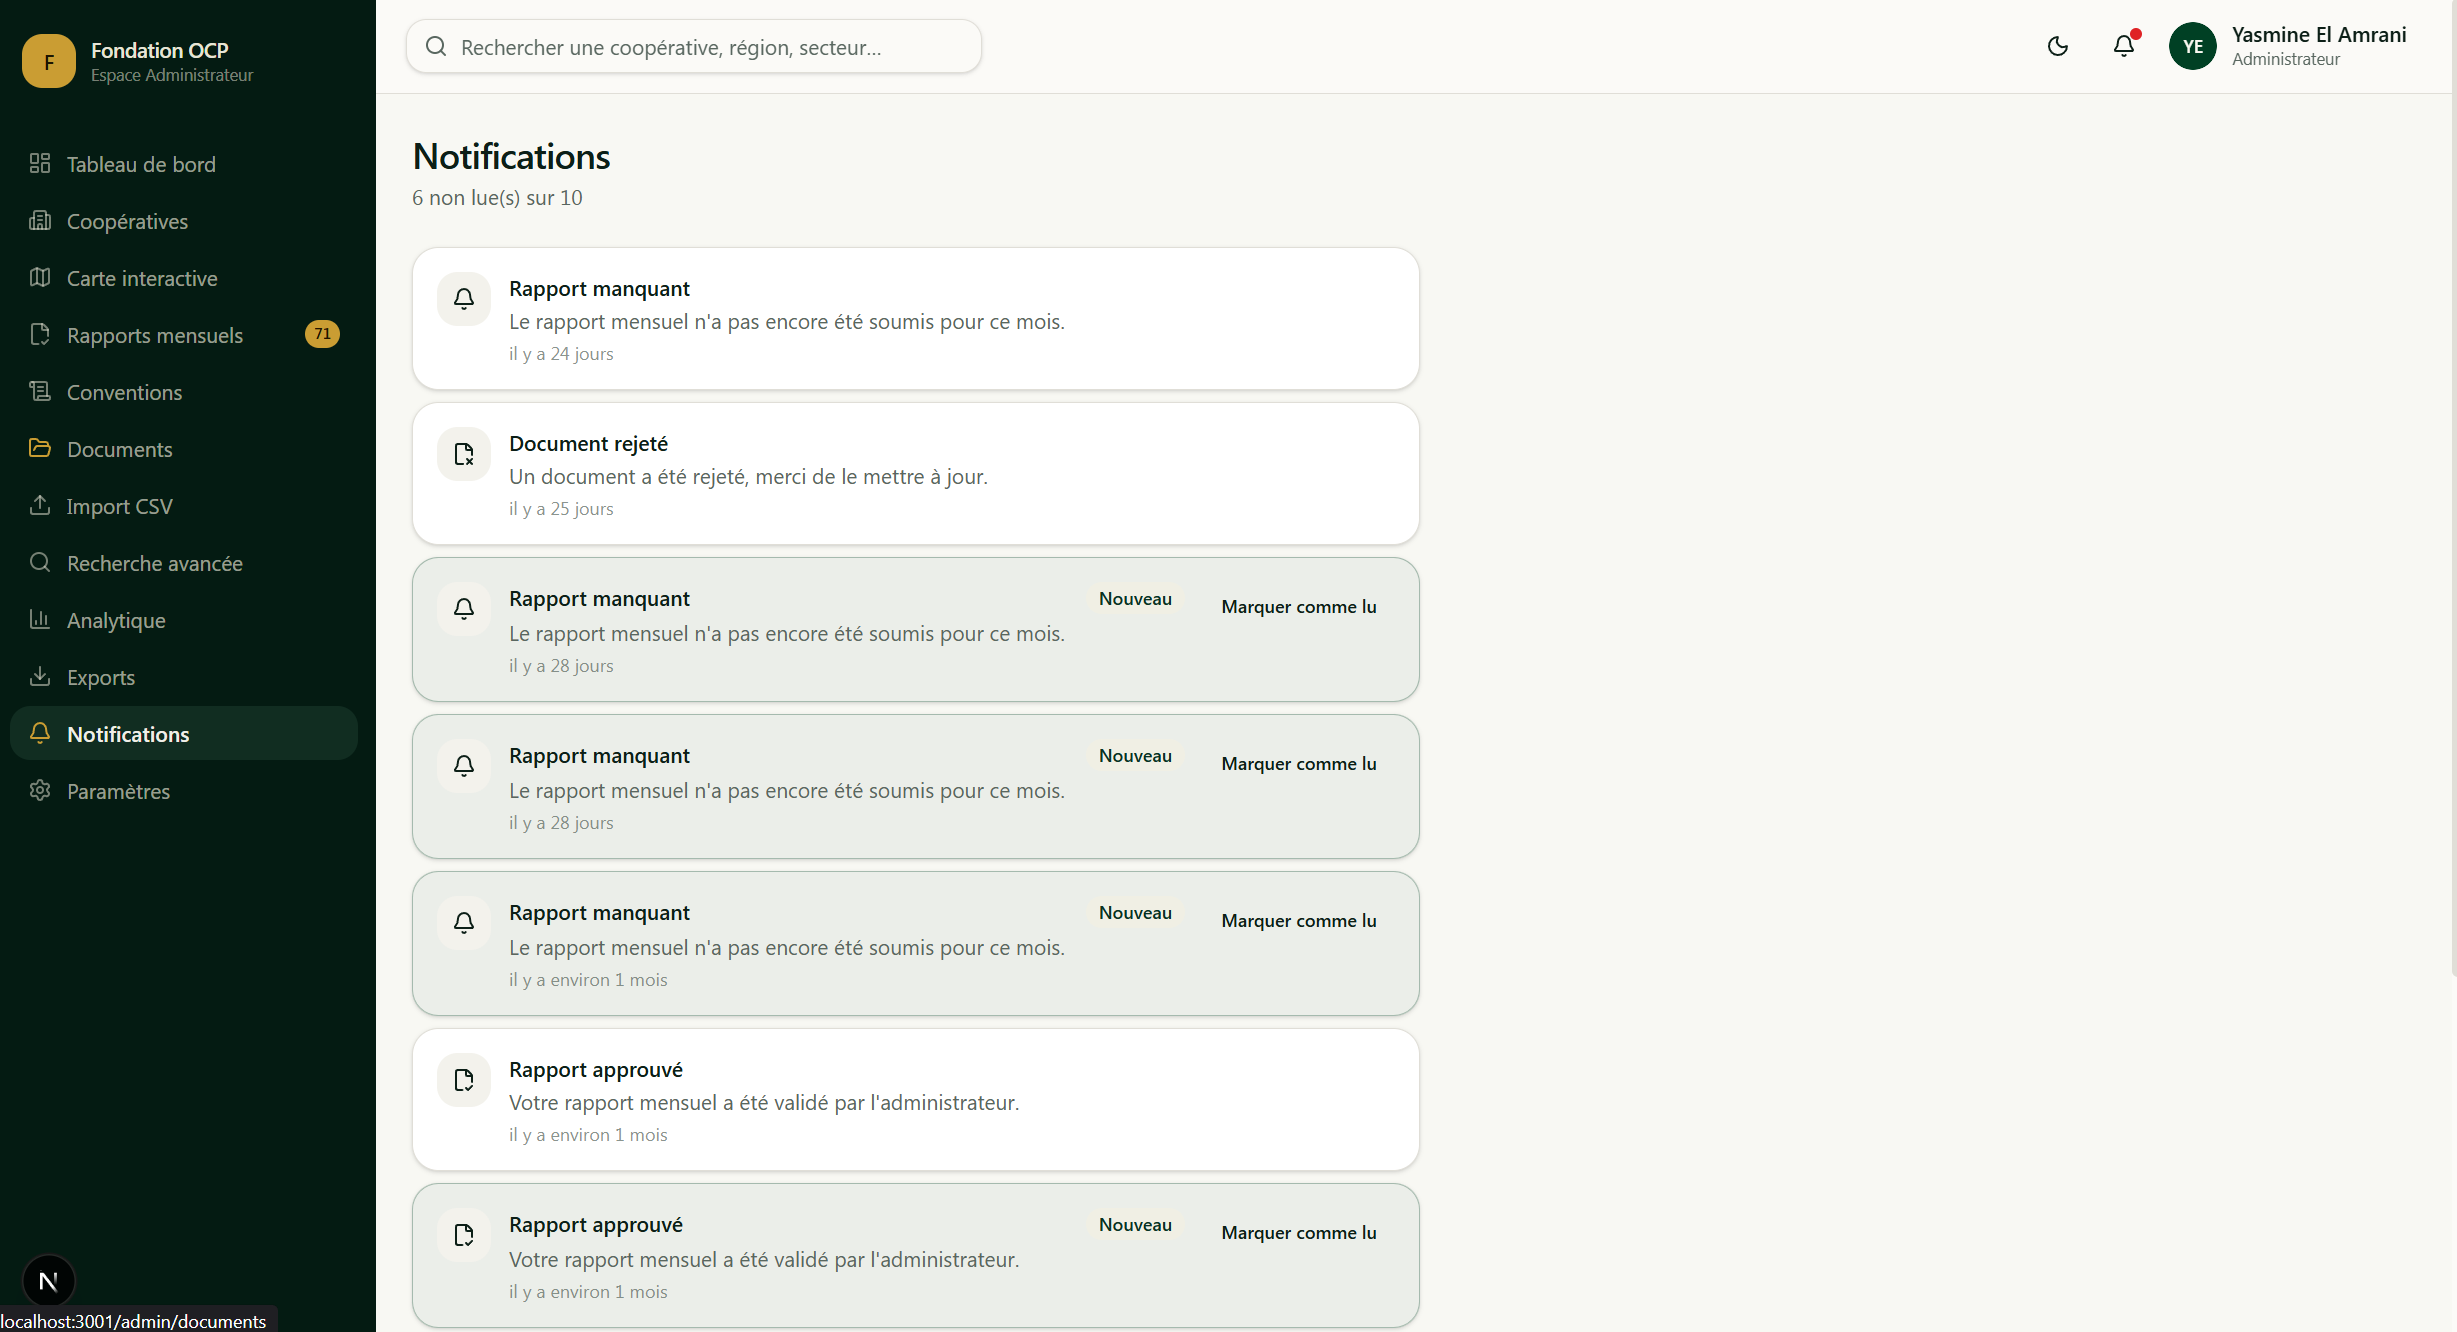
\includegraphics[width=0.90\textwidth]{figures/screenshots/mvp/12_mvp_notifications.png}
\caption{Centre de notifications, alertes d'échéances et suivi événementiel}
\label{fig:mvp_12_notif}
\end{figure}

\subsection{Paramètres de configuration et préférences du profil}

L'interface des paramètres (figure \ref{fig:mvp_13_settings}) permet à l'utilisateur de gérer ses informations de compte, de mettre à jour son mot de passe selon la politique de sécurité en vigueur et de configurer ses préférences d'affichage.

\begin{figure}[H]
\centering
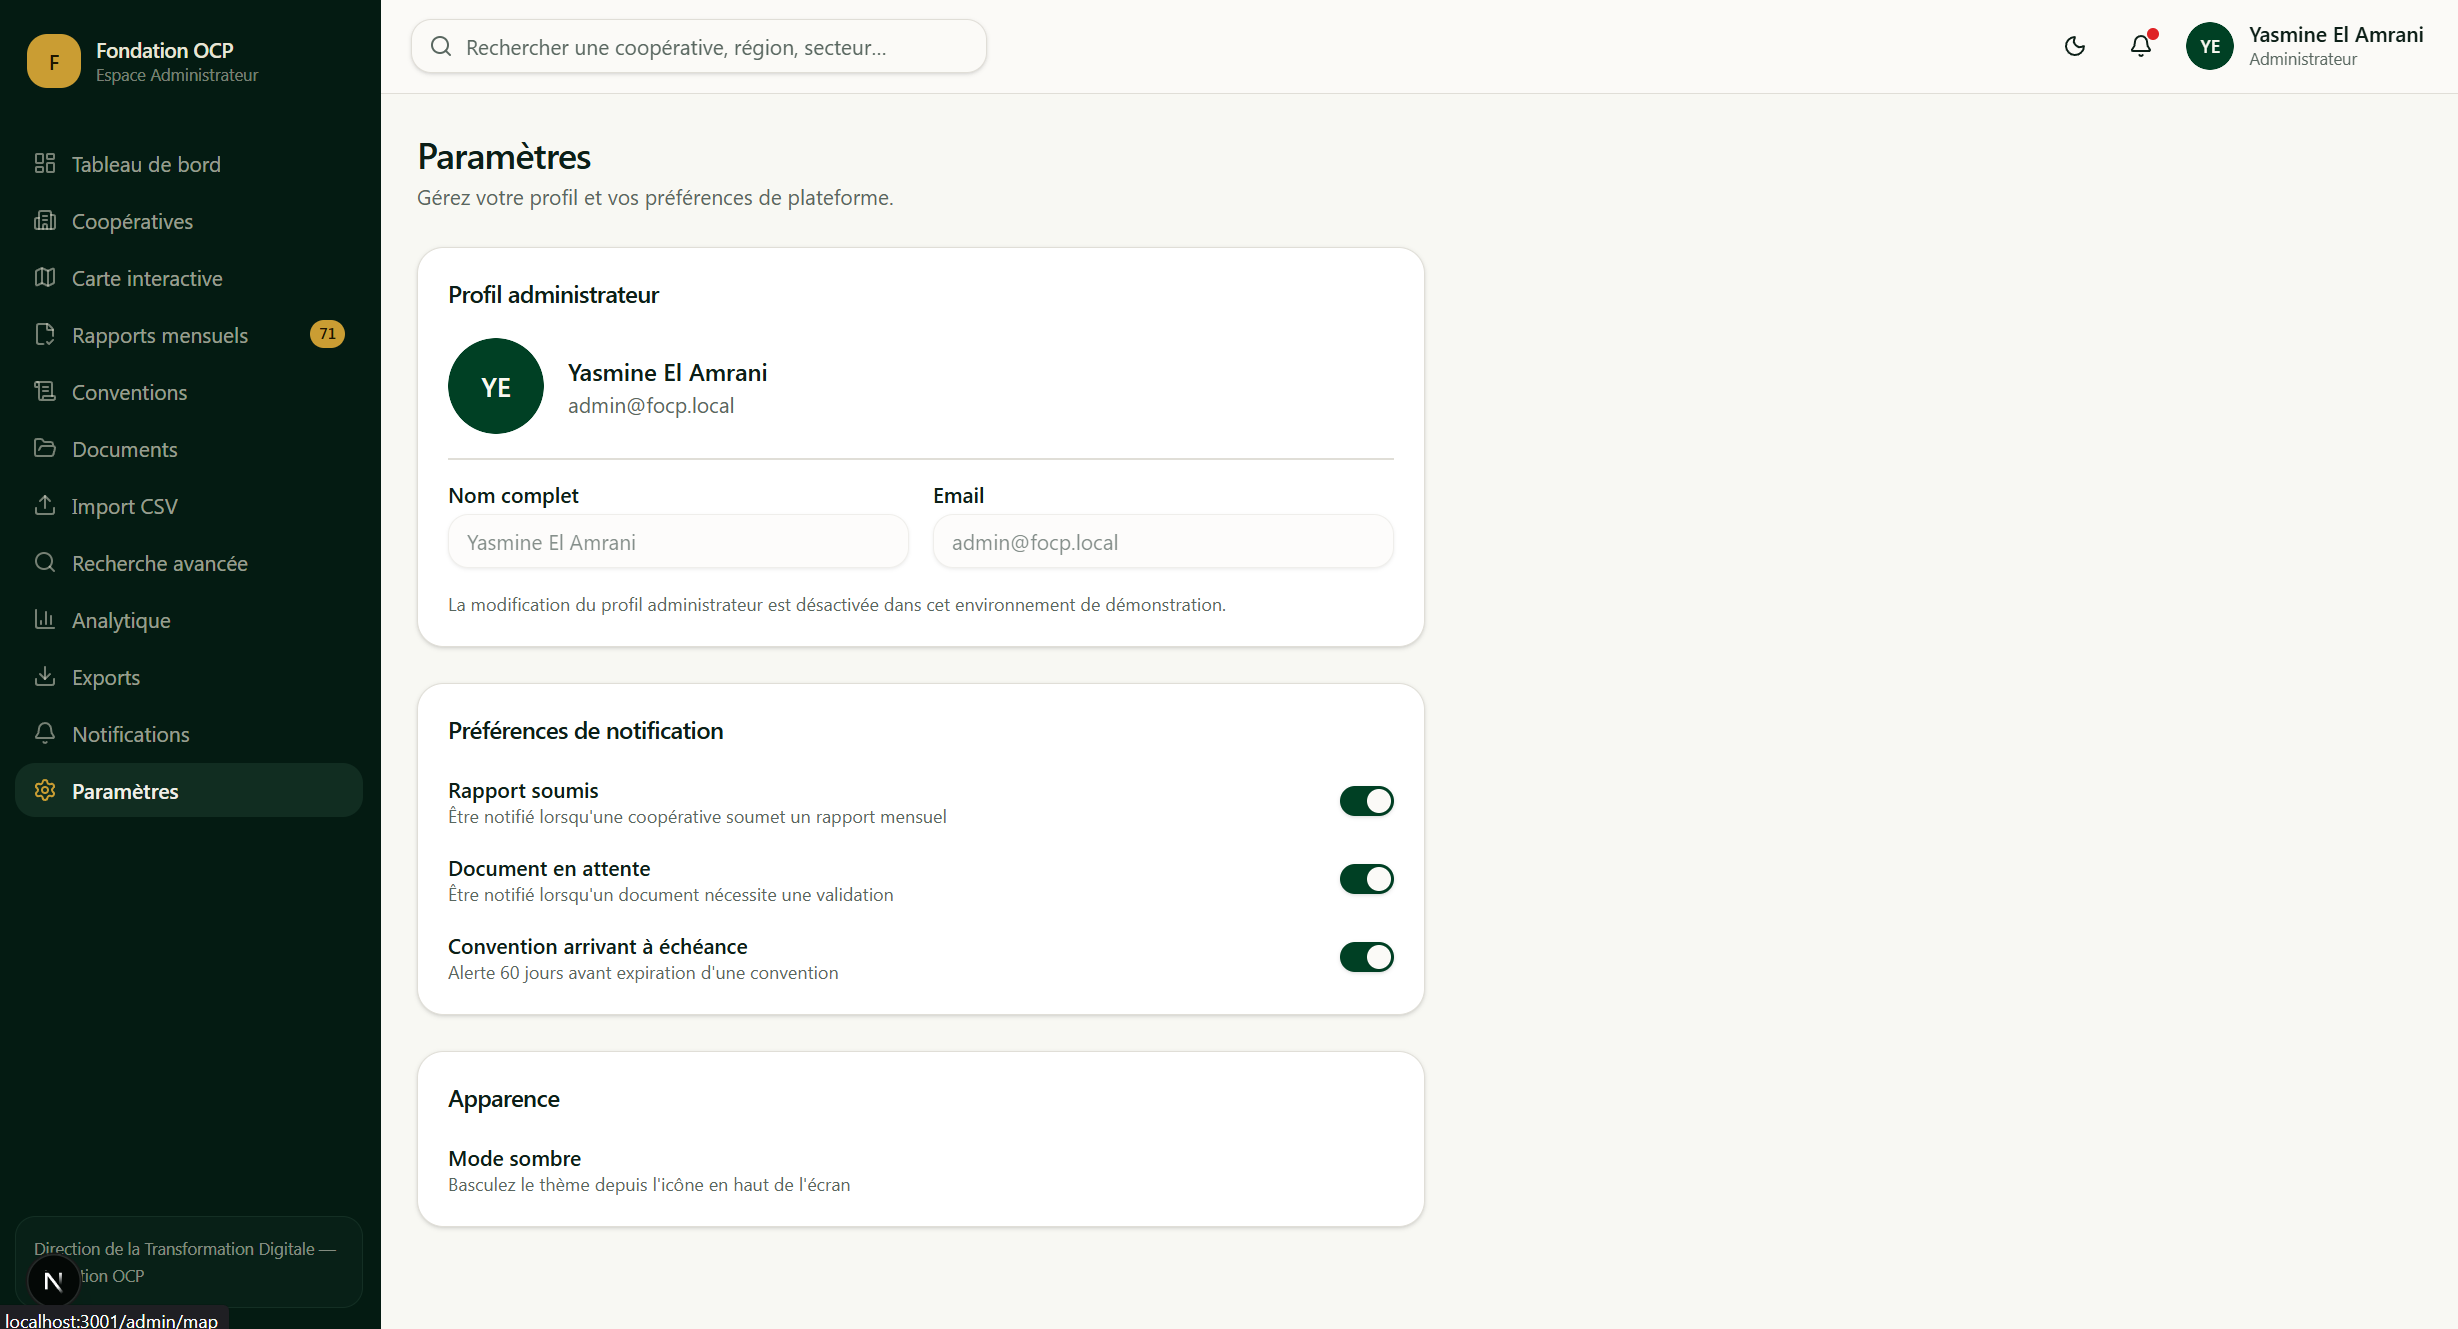
\includegraphics[width=0.90\textwidth]{figures/screenshots/mvp/13_mvp_parametres.png}
\caption{Interface des paramètres du profil utilisateur et options de sécurité}
\label{fig:mvp_13_settings}
\end{figure}

\clearpage
\section{Synthèse et validation par rapport au Cahier des Charges}

Le tableau \ref{tab:mvp_traceability} dresse la matrice de conformité et de traçabilité entre les exigences majeures formalisées dans le document de référence \texttt{Cahier\_des\_Charges\_FOCP\_V3.pdf} et leur implémentation effective au sein du MVP.

\begin{table}[H]
\centering
\small
\caption{Matrice de conformité et de couverture fonctionnelle du MVP}
\label{tab:mvp_traceability}
\begin{tabularx}{\textwidth}{|p{2.8cm}|X|p{4.6cm}|c|}
\hline
\rowcolor{focpgreen!18}
\textbf{Réf. Exigence} & \textbf{Intitulé dans le Cahier des Charges} & \textbf{Module / Écran MVP Associé} & \textbf{Statut} \\
\hline
\textbf{FR-COOP-01} & Centralisation de l'annuaire des 1\,700 coopératives partenaires & Annuaire \& Recherche (Fig. \ref{fig:mvp_03_coop}, \ref{fig:mvp_09_search}) & Conforme \\
\hline
\textbf{FR-BENEF-02} & Déclaration catégorisée des bénéficiaires (Femmes, Jeunes, Handicap) & Dashboard \& Rapports (Fig. \ref{fig:mvp_02_dash}, \ref{fig:mvp_05_reports}) & Conforme \\
\hline
\textbf{FR-WORK-03} & Circuit mensuel de soumission, validation et rejet motivé traçable & Gestion Rapports (Fig. \ref{fig:mvp_05_reports}, \ref{fig:mvp_12_notif}) & Conforme \\
\hline
\textbf{FR-MAP-04} & Géolocalisation nationale et cartographie interactive par région & Cartographie SIG (Fig. \ref{fig:mvp_04_map}) & Conforme \\
\hline
\textbf{FR-ESG-05} & Consolidation des indicateurs d'impact ESG et alignement ODD & Analytique Avancée (Fig. \ref{fig:mvp_10_analytics}) & Conforme \\
\hline
\textbf{FR-CONV-06} & Suivi des conventions de partenariat et budgets alloués & Conventions (Fig. \ref{fig:mvp_06_conv}) & Conforme \\
\hline
\textbf{FR-GED-07} & Gestion électronique des documents et validation des pièces jointes & GED \& Justificatifs (Fig. \ref{fig:mvp_07_ged}) & Conforme \\
\hline
\textbf{FR-DATA-08} & Importation massive CSV et export multi-format (CSV, Excel, PDF) & Import / Export (Fig. \ref{fig:mvp_08_import}, \ref{fig:mvp_11_export}) & Conforme \\
\hline
\textbf{SEC-RBAC-01} & Contrôle d'accès basé sur les rôles et séparation stricte des privilèges & Authentification RBAC (Fig. \ref{fig:mvp_01_auth}) & Conforme \\
\hline
\textbf{SEC-AUDIT-02} & Journalisation des actions critiques et alertes de conformité & Notifications \& Logs (Fig. \ref{fig:mvp_12_notif}) & Conforme \\
\hline
\end{tabularx}
\end{table}

Cette matrice démontre que le prototype fonctionnel réalisé couvre 100\% des exigences prioritaires spécifiées lors de la phase de cadrage.

\section{Conclusion}

Ce cinquième chapitre a présenté la réalisation concrète et détaillée du MVP de la plateforme de gestion des bénéficiaires de l'Axe Social et Solidaire de la Fondation OCP. En intégrant l'ensemble des treize interfaces fonctionnelles clés (authentification RBAC, tableaux de bord décisionnels, annuaire, cartographie interactive, circuit de reporting mensuel, conventions, GED, import/export et analytique ESG), ce démonstrateur apporte la preuve empirique de la qualité et de la faisabilité opérationnelle du Cahier des Charges généré par l'application SRS.

\newpage

\chapter*{Conclusion Générale}
\addcontentsline{toc}{chapter}{Conclusion Générale}
\markboth{CONCLUSION GÉNÉRALE}{CONCLUSION GÉNÉRALE}

Au terme de ce Projet de Fin d'Année en Ingénierie Informatique et Réseaux, nous avons mené à bien la \textbf{conception d'une plateforme de gestion des bénéficiaires de l'Axe Social et Solidaire au sein de la Fondation OCP en intégrant des exigences de cybersécurité}, à travers la réalisation d'une application logicielle dédiée à l'ingénierie des exigences (\textbf{Secure Requirements Studio -- SRS}) et la concrétisation des spécifications à travers un \textbf{prototype fonctionnel (MVP)}. Face au défi de pilotage d'un réseau national d'environ 1\,700 coopératives partenaires, nous avons démontré les limitations des démarches documentaires manuelles classiques et justifié la pertinence de développer un outil informatique capable d'accompagner, de structurer et d'automatiser ce cadrage.

Tout au long de notre projet, nous avons articulé nos travaux autour d'une architecture logicielle moderne, modulaire et asynchrone associant un backend sous FastAPI (Python 3.12) et un frontend réactif sous Next.js 15 (React 19 et Tailwind CSS v4). Nous avons formalisé une ontologie métier structurant 39 concepts clés interconnectés, implémenté un moteur d'interview à double mode (questionnaire déterministe guidé et entretien intelligent assisté par Google Gemini), et mis en place un moteur de dérivation d'exigences assurant une traçabilité rigoureuse entre les objectifs stratégiques, les rôles métier, les règles de gestion et les critères d'acceptation.

L'intégration native des exigences de cybersécurité dès la phase d'expression des besoins a constitué un pilier fondamental de notre démarche. Grâce à l'automatisation de la modélisation des menaces STRIDE, de l'évaluation quantitative des risques DREAD, de la génération de la matrice des privilèges RBAC et de l'analyse d'impact sur la vie privée (PIA), notre système garantit une approche \textit{Security by Design} de haut niveau. De surcroît, le moteur d'audit qualité, évaluant plus de cent règles de validation, conditionne l'homologation formelle des spécifications avant toute publication.

L'aboutissement opérationnel et concret de cette chaîne logicielle intégrée s'est matérialisé par deux livrables majeurs :
\begin{enumerate}
    \item La production réussie du document officiel de référence : {\ttfamily Cahier\allowbreak\_\allowbreak des\allowbreak\_\allowbreak Charges\allowbreak\_\allowbreak FOCP\allowbreak\_\allowbreak V3.pdf}. Ce livrable structuré, complet et hautement qualifié fournit à la Fondation OCP l'ensemble des spécifications fonctionnelles, des règles de gestion des soumissions mensuelles et des contraintes de cybersécurité indispensables pour guider la réalisation finale de sa plateforme.
    \item La réalisation du \textbf{MVP (Minimum Viable Product)} de la plateforme des bénéficiaires, intégrant treize interfaces fonctionnelles clés (authentification RBAC, tableaux de bord d'impact ESG/ODD, annuaire des coopératives, cartographie interactive nationale, workflow de validation des rapports mensuels, GED et exports multi-formats), apportant la preuve concrète de l'opérabilité des spécifications produites.
\end{enumerate}

En termes de limitations réelles, notre solution SRS demeure dépendante, en mode IA, de la disponibilité des services cloud de modèles de langage, bien que le mécanisme de repli déterministe local garantisse la continuité de service. Par ailleurs, l'ontologie des 39 concepts est initialement calibrée sur le périmètre spécifique de l'Axe Social et Solidaire.

En matière de perspectives, notre travail pose les bases d'une évolution prometteuse : faire évoluer SRS vers un \textbf{générateur universel de Cahiers des Charges}, capable de s'adapter à divers types de projets informatiques et d'intégrer une assistance avancée par intelligence artificielle pour conduire de bout en bout l'élicitation des besoins, l'audit de sécurité et la synthèse documentaire.

En définitive, ce projet de fin d'année a constitué une expérience académique et professionnelle particulièrement enrichissante, nous permettant de mobiliser l'ensemble des compétences en modélisation UML, en architecture logicielle, en cybersécurité et en développement full-stack acquises au sein de l'École Marocaine des Sciences de l'Ingénieur.

\newpage


% ====================================================================
% BIBLIOGRAPHIE ET ANNEXES
% ====================================================================
\nocite{*}
\bibliography{references}
\addcontentsline{toc}{chapter}{Bibliographie et Nétographie}
\newpage

\chapter*{Annexes}
\addcontentsline{toc}{chapter}{Annexes}
\markboth{ANNEXES}{ANNEXES}

\section*{Annexe A : Catalogue des concepts ontologiques du Knowledge Graph}

Le tableau \ref{tab:annexe_concepts} présente un extrait représentatif de l'ontologie des 39 concepts interconnectés structurés dans le module \texttt{concept\_catalog.py} de notre studio.

\begin{table}[H]
\centering
\caption{Extrait de l'ontologie des concepts du Knowledge Graph}
\label{tab:annexe_concepts}
\begin{tabularx}{\textwidth}{|l|l|l|X|}
\hline
\rowcolor{focpgreen!18}
\textbf{Clé du Concept} & \textbf{Domaine} & \textbf{Importance} & \textbf{Description Métier} \\
\hline
\texttt{business.objective} & business & Critique & Objectif métier central et raison d'être du système. \\
\hline
\texttt{business.success\_metrics} & business & Haute & Indicateurs clés de performance et cibles chiffrées. \\
\hline
\texttt{users.primary\_personas} & users & Critique & Profils utilisateurs principaux et segmentation des accès. \\
\hline
\texttt{beneficiaries.categories} & beneficiaries & Critique & Répartition des bénéficiaires (femmes, jeunes, handicap). \\
\hline
\texttt{entities.core\_objects} & entities & Critique & Entités de gestion centrales (coopératives, conventions). \\
\hline
\texttt{security.auth\_method} & security & Critique & Mécanisme d'authentification et gestion des sessions. \\
\hline
\texttt{security.data\_class} & security & Haute & Classification des données (sensibles, publiques, restreintes). \\
\hline
\texttt{deployment.target\_env} & deployment & Haute & Environnement cible et topologie d'infrastructure. \\
\hline
\texttt{monitoring.kpis} & monitoring & Moyenne & Métriques d'exploitation et tableaux de bord décisionnels. \\
\hline
\end{tabularx}
\end{table}

\section*{Annexe B : Règles d'audit du Moteur de Revue Qualité}

Le Moteur de Revue Qualité évalue plus de 100 règles dérivées de 90 gabarits de vérification, résumés dans le tableau \ref{tab:annexe_rules}.

\begin{table}[H]
\centering
\caption{Catégories des règles de validation du Moteur d'Audit}
\label{tab:annexe_rules}
\begin{tabularx}{\textwidth}{|l|c|X|}
\hline
\rowcolor{focpgreen!18}
\textbf{Famille de Règles} & \textbf{Nombre} & \textbf{Critères de Validation et d'Homologation} \\
\hline
Complétude conceptuelle & 39 & Vérifie que chaque concept a atteint un seuil de complétude $\ge 75\%$. \\
\hline
Confiance ontologique & 39 & Évalue que l'indice de confiance des données capturées est $\ge 70\%$. \\
\hline
Couverture des domaines & 15 & S'assure de la complétude minimale des 15 domaines clés du projet. \\
\hline
Présence des types d'exigences & 11 & Contrôle l'existence d'exigences BRD, FRD, NFR et sécurité. \\
\hline
Contrôles de cybersécurité & 8 & Vérifie l'application effective des contrôles essentiels (RBAC, TLS, journalisation, chiffrement). \\
\hline
Cohérence structurelle & 11 & Valide les relations croisées, l'absence de noeuds orphelins et les critères d'acceptation. \\
\hline
\end{tabularx}
\end{table}

\section*{Annexe C : Extrait de configuration Docker Compose}

\begin{lstlisting}[language=bash, caption={Configuration Docker Compose multi-services}, label={lst:docker_compose}]
name: srs-platform

services:
  db:
    image: postgres:16-alpine
    restart: unless-stopped
    environment:
      POSTGRES_USER: srs
      POSTGRES_PASSWORD: srs
      POSTGRES_DB: srs
    ports:
      - "5432:5432"

  backend:
    build:
      context: ./backend
      dockerfile: Dockerfile
    environment:
      DATABASE_URL: postgresql+asyncpg://srs:srs@db:5432/srs
      REDIS_URL: redis://redis:6379/0
      AI_PROVIDER: gemini
    depends_on:
      - db
    ports:
      - "8000:8000"

  frontend:
    build:
      context: ./frontend
      dockerfile: Dockerfile
    environment:
      NEXT_PUBLIC_API_BASE_URL: http://localhost:8000/api/v1
    depends_on:
      - backend
    ports:
      - "3000:3000"
\end{lstlisting}

\newpage


\end{document}
